\documentclass[twoside]{book}

% Packages required by doxygen
\usepackage{fixltx2e}
\usepackage{calc}
\usepackage{doxygen}
\usepackage[export]{adjustbox} % also loads graphicx
\usepackage{graphicx}
\usepackage[utf8]{inputenc}
\usepackage{makeidx}
\usepackage{multicol}
\usepackage{multirow}
\PassOptionsToPackage{warn}{textcomp}
\usepackage{textcomp}
\usepackage[nointegrals]{wasysym}
\usepackage[table]{xcolor}

% Font selection
\usepackage[T1]{fontenc}
\usepackage[scaled=.90]{helvet}
\usepackage{courier}
\usepackage{amssymb}
\usepackage{sectsty}
\renewcommand{\familydefault}{\sfdefault}
\allsectionsfont{%
  \fontseries{bc}\selectfont%
  \color{darkgray}%
}
\renewcommand{\DoxyLabelFont}{%
  \fontseries{bc}\selectfont%
  \color{darkgray}%
}
\newcommand{\+}{\discretionary{\mbox{\scriptsize$\hookleftarrow$}}{}{}}

% Page & text layout
\usepackage{geometry}
\geometry{%
  a4paper,%
  top=2.5cm,%
  bottom=2.5cm,%
  left=2.5cm,%
  right=2.5cm%
}
\tolerance=750
\hfuzz=15pt
\hbadness=750
\setlength{\emergencystretch}{15pt}
\setlength{\parindent}{0cm}
\setlength{\parskip}{3ex plus 2ex minus 2ex}
\makeatletter
\renewcommand{\paragraph}{%
  \@startsection{paragraph}{4}{0ex}{-1.0ex}{1.0ex}{%
    \normalfont\normalsize\bfseries\SS@parafont%
  }%
}
\renewcommand{\subparagraph}{%
  \@startsection{subparagraph}{5}{0ex}{-1.0ex}{1.0ex}{%
    \normalfont\normalsize\bfseries\SS@subparafont%
  }%
}
\makeatother

% Headers & footers
\usepackage{fancyhdr}
\pagestyle{fancyplain}
\fancyhead[LE]{\fancyplain{}{\bfseries\thepage}}
\fancyhead[CE]{\fancyplain{}{}}
\fancyhead[RE]{\fancyplain{}{\bfseries\leftmark}}
\fancyhead[LO]{\fancyplain{}{\bfseries\rightmark}}
\fancyhead[CO]{\fancyplain{}{}}
\fancyhead[RO]{\fancyplain{}{\bfseries\thepage}}
\fancyfoot[LE]{\fancyplain{}{}}
\fancyfoot[CE]{\fancyplain{}{}}
\fancyfoot[RE]{\fancyplain{}{\bfseries\scriptsize Generated by Doxygen }}
\fancyfoot[LO]{\fancyplain{}{\bfseries\scriptsize Generated by Doxygen }}
\fancyfoot[CO]{\fancyplain{}{}}
\fancyfoot[RO]{\fancyplain{}{}}
\renewcommand{\footrulewidth}{0.4pt}
\renewcommand{\chaptermark}[1]{%
  \markboth{#1}{}%
}
\renewcommand{\sectionmark}[1]{%
  \markright{\thesection\ #1}%
}

% Indices & bibliography
\usepackage{natbib}
\usepackage[titles]{tocloft}
\setcounter{tocdepth}{3}
\setcounter{secnumdepth}{5}
\makeindex

% Hyperlinks (required, but should be loaded last)
\usepackage{ifpdf}
\ifpdf
  \usepackage[pdftex,pagebackref=true]{hyperref}
\else
  \usepackage[ps2pdf,pagebackref=true]{hyperref}
\fi
\hypersetup{%
  colorlinks=true,%
  linkcolor=blue,%
  citecolor=blue,%
  unicode%
}

% Custom commands
\newcommand{\clearemptydoublepage}{%
  \newpage{\pagestyle{empty}\cleardoublepage}%
}

\usepackage{caption}
\captionsetup{labelsep=space,justification=centering,font={bf},singlelinecheck=off,skip=4pt,position=top}

%===== C O N T E N T S =====

\begin{document}

% Titlepage & ToC
\hypersetup{pageanchor=false,
             bookmarksnumbered=true,
             pdfencoding=unicode
            }
\pagenumbering{alph}
\begin{titlepage}
\vspace*{7cm}
\begin{center}%
{\Large C\+Linter }\\
\vspace*{1cm}
{\large Generated by Doxygen 1.8.13}\\
\end{center}
\end{titlepage}
\clearemptydoublepage
\pagenumbering{roman}
\tableofcontents
\clearemptydoublepage
\pagenumbering{arabic}
\hypersetup{pageanchor=true}

%--- Begin generated contents ---
\chapter{C\+Linter}
\label{index}\hypertarget{index}{}Linter in C \section*{To compile}

make \section*{To run one file}

./linter

or

./linter \mbox{[}path/to/config/file\mbox{]}

\section*{To run tests}

./test.sh

\section*{T\+O\+DO\+:}


\begin{DoxyItemize}
\item Delimiter les tokens (Mot clés, délimiteurs, opérateurs, noms variables, espaces, reste?) \+:+1\+: \+:-\/1\+:
\item Partie 1\+:
\begin{DoxyItemize}
\item \mbox{[}x\mbox{]} Récursif sur les dossiers
\item \mbox{[}x\mbox{]} Charger récursivement les fichiers de configuration
\end{DoxyItemize}
\item Règles\+:
\begin{DoxyItemize}
\item \mbox{[}x\mbox{]} array-\/bracket-\/eol
\item \mbox{[}x\mbox{]} operators-\/spacing
\item \mbox{[} \mbox{]} indent
\item \mbox{[}x\mbox{]} comments-\/header
\item \mbox{[}x\mbox{]} max-\/line-\/numbers
\item \mbox{[}x\mbox{]} max-\/file-\/line-\/numbers
\item \mbox{[}x\mbox{]} no-\/trailing-\/spaces
\item \mbox{[}x\mbox{]} no-\/multi-\/declaration
\item \mbox{[} \mbox{]} unused-\/variable
\item \mbox{[} \mbox{]} undeclared-\/variable
\item \mbox{[} \mbox{]} no-\/prototype
\item \mbox{[} \mbox{]} unused-\/function
\item \mbox{[} \mbox{]} undeclared-\/function
\item \mbox{[} \mbox{]} variable-\/assignment-\/type
\item \mbox{[} \mbox{]} function-\/parameters-\/type 
\end{DoxyItemize}
\end{DoxyItemize}
\chapter{Class Index}
\section{Class List}
Here are the classes, structs, unions and interfaces with brief descriptions\+:\begin{DoxyCompactList}
\item\contentsline{section}{\hyperlink{structConfig__t}{Config\+\_\+t} \\*Structure to store all configurations elements }{\pageref{structConfig__t}}{}
\item\contentsline{section}{\hyperlink{structToken__t}{Token\+\_\+t} \\*Structure to store a Token }{\pageref{structToken__t}}{}
\end{DoxyCompactList}

\chapter{File Index}
\section{File List}
Here is a list of all files with brief descriptions\+:\begin{DoxyCompactList}
\item\contentsline{section}{/home/a4742849/\+Documents/\+C\+Linter/src/\hyperlink{changeType_8c}{change\+Type.\+c} \\*This c file will contain all functions to change type of a token }{\pageref{changeType_8c}}{}
\item\contentsline{section}{/home/a4742849/\+Documents/\+C\+Linter/src/\hyperlink{changeType_8h}{change\+Type.\+h} \\*This header file will contain all required definitions and basic utilities functions to change type of a token }{\pageref{changeType_8h}}{}
\item\contentsline{section}{/home/a4742849/\+Documents/\+C\+Linter/src/\hyperlink{checkCoding_8c}{check\+Coding.\+c} \\*This c file will contain all functions to check simple coding style rules }{\pageref{checkCoding_8c}}{}
\item\contentsline{section}{/home/a4742849/\+Documents/\+C\+Linter/src/\hyperlink{checkCoding_8h}{check\+Coding.\+h} \\*This header file will contain all required definitions and basic utilities functions to check rules on a C file }{\pageref{checkCoding_8h}}{}
\item\contentsline{section}{/home/a4742849/\+Documents/\+C\+Linter/src/\hyperlink{checker_8c}{checker.\+c} \\*This c file will contain all functions to check a grammar }{\pageref{checker_8c}}{}
\item\contentsline{section}{/home/a4742849/\+Documents/\+C\+Linter/src/\hyperlink{checker_8h}{checker.\+h} \\*This header file will contain all required definitions and basic utilities functions to check grammar of a C file }{\pageref{checker_8h}}{}
\item\contentsline{section}{/home/a4742849/\+Documents/\+C\+Linter/src/\hyperlink{checkVarFunc_8c}{check\+Var\+Func.\+c} \\*This c file will contain all functions to check rules on functions or variables }{\pageref{checkVarFunc_8c}}{}
\item\contentsline{section}{/home/a4742849/\+Documents/\+C\+Linter/src/\hyperlink{checkVarFunc_8h}{check\+Var\+Func.\+h} \\*This header file will contain all required definitions and basic utilities functions to check rules on functions or variables on a C file }{\pageref{checkVarFunc_8h}}{}
\item\contentsline{section}{/home/a4742849/\+Documents/\+C\+Linter/src/\hyperlink{config_8c}{config.\+c} \\*This c file will contain all functions to load a lconf file }{\pageref{config_8c}}{}
\item\contentsline{section}{/home/a4742849/\+Documents/\+C\+Linter/src/\hyperlink{config_8h}{config.\+h} \\*This header file will contain all required definitions and basic utilities functions to read and load a configuration file }{\pageref{config_8h}}{}
\item\contentsline{section}{/home/a4742849/\+Documents/\+C\+Linter/src/\hyperlink{files_8c}{files.\+c} \\*This c file will contain all functions to load a file in a char$\ast$$\ast$ }{\pageref{files_8c}}{}
\item\contentsline{section}{/home/a4742849/\+Documents/\+C\+Linter/src/\hyperlink{files_8h}{files.\+h} \\*This header file will contain all required definitions and basic utilities functions to read and load a file into a char$\ast$$\ast$ }{\pageref{files_8h}}{}
\item\contentsline{section}{/home/a4742849/\+Documents/\+C\+Linter/src/\hyperlink{freeAll_8c}{free\+All.\+c} \\*This c file will contain all functions to free all structures and pointers }{\pageref{freeAll_8c}}{}
\item\contentsline{section}{/home/a4742849/\+Documents/\+C\+Linter/src/\hyperlink{freeAll_8h}{free\+All.\+h} \\*This header file will contain all required definitions and basic utilities functions to free the memory of the program }{\pageref{freeAll_8h}}{}
\item\contentsline{section}{/home/a4742849/\+Documents/\+C\+Linter/src/\hyperlink{headers_8h}{headers.\+h} \\*This header file will contain all required definitions and basic header files for main function }{\pageref{headers_8h}}{}
\item\contentsline{section}{/home/a4742849/\+Documents/\+C\+Linter/src/\hyperlink{listFiles_8c}{list\+Files.\+c} \\*This c file will contain all functions to list files we want to work on }{\pageref{listFiles_8c}}{}
\item\contentsline{section}{/home/a4742849/\+Documents/\+C\+Linter/src/\hyperlink{listFiles_8h}{list\+Files.\+h} \\*This header file will contain all required definitions and basic utilities functions to check grammar of a C file }{\pageref{listFiles_8h}}{}
\item\contentsline{section}{/home/a4742849/\+Documents/\+C\+Linter/src/\hyperlink{main_8c}{main.\+c} \\*This c file will contain all the logic to analyze and warn a user of it\textquotesingle{}s bad C type skills }{\pageref{main_8c}}{}
\item\contentsline{section}{/home/a4742849/\+Documents/\+C\+Linter/src/\hyperlink{parser_8c}{parser.\+c} \\*This c file will contain all functions to parse a file }{\pageref{parser_8c}}{}
\item\contentsline{section}{/home/a4742849/\+Documents/\+C\+Linter/src/\hyperlink{parser_8h}{parser.\+h} \\*This header file will contain all required definitions and basic utilities functions to transform text into Tokens }{\pageref{parser_8h}}{}
\item\contentsline{section}{/home/a4742849/\+Documents/\+C\+Linter/src/\hyperlink{token_8c}{token.\+c} \\*This c file will contain all functions to create a Token }{\pageref{token_8c}}{}
\item\contentsline{section}{/home/a4742849/\+Documents/\+C\+Linter/src/\hyperlink{token_8h}{token.\+h} \\*This header file will contain all required definitions and basic utilities functions to create a Token }{\pageref{token_8h}}{}
\item\contentsline{section}{/home/a4742849/\+Documents/\+C\+Linter/src/\hyperlink{tool_8c}{tool.\+c} \\*This c file will contain all functions for various tools }{\pageref{tool_8c}}{}
\item\contentsline{section}{/home/a4742849/\+Documents/\+C\+Linter/src/\hyperlink{tool_8h}{tool.\+h} \\*This header file will contain all required definitions and basic utilities functions to print, check token\textquotesingle{}s nature }{\pageref{tool_8h}}{}
\end{DoxyCompactList}

\chapter{Class Documentation}
\hypertarget{structConfig__t}{}\section{Config\+\_\+t Struct Reference}
\label{structConfig__t}\index{Config\+\_\+t@{Config\+\_\+t}}


Structure to store all configurations elements.  




{\ttfamily \#include $<$config.\+h$>$}

\subsection*{Public Attributes}
\begin{DoxyCompactItemize}
\item 
char $\ast$ \hyperlink{structConfig__t_a1dd391e253a5a3bc3d27bb986977f593}{extends}
\item 
short \hyperlink{structConfig__t_a638fad6042df80f4ddef34593654dd9d}{array\+Bracket\+Eol}
\item 
short \hyperlink{structConfig__t_a358f05ff06ff962ffac4573d120d52a5}{operators\+Spacing}
\item 
short \hyperlink{structConfig__t_a65d13a772c2b16fdcf47404c4eca2c70}{comma\+Spacing}
\item 
short \hyperlink{structConfig__t_a9812b0788540b97410f06ca3c449f4f9}{indent}
\item 
short \hyperlink{structConfig__t_af39c67047e4a3554d6a3ee63fe557835}{comments\+Header}
\item 
short \hyperlink{structConfig__t_a1396cdd37b3769c1e7acc8421fc6299f}{max\+Line\+Numbers}
\item 
short \hyperlink{structConfig__t_a0cdf48abfd86bbec74f265ae23bf47fe}{max\+File\+Line\+Numbers}
\item 
short \hyperlink{structConfig__t_ad284d677c7abe2aa97d7eb01082e264d}{no\+Tralling\+Spaces}
\item 
short \hyperlink{structConfig__t_a2d4508be47969205d76d73c1f2658e3a}{No\+Multi\+Declaration}
\item 
short \hyperlink{structConfig__t_af2c9852fc94e9d3ae2cd54f5750dd37f}{unused\+Variable}
\item 
short \hyperlink{structConfig__t_a704e6830c0e2d93a5441300ae6592aec}{undeclared\+Variable}
\item 
short \hyperlink{structConfig__t_a9ab1cbe58615ccaab6479f4ef607d3f4}{no\+Prototype}
\item 
short \hyperlink{structConfig__t_aa2d06bad2fc7b51d26e0bae0032c4da3}{unused\+Function}
\item 
short \hyperlink{structConfig__t_ae10b1d04c6d0762fbcb7b4406d888a5d}{undeclared\+Function}
\item 
short \hyperlink{structConfig__t_abed8ad04a1696c089ba4ce283743c67e}{variable\+Assignment\+Type}
\item 
short \hyperlink{structConfig__t_ac839f0c65179233fc86b731cac821023}{function\+Parameters\+Type}
\item 
char $\ast$$\ast$ \hyperlink{structConfig__t_a63665db6545b70d0c856041075352f6f}{excluded\+Files}
\item 
int \hyperlink{structConfig__t_ab97fb08912a0271b7b4623a75c6b1fda}{nb\+Excluded\+Files}
\item 
short \hyperlink{structConfig__t_a983242633069db53f8ce1852ee8eabfc}{recursive}
\end{DoxyCompactItemize}


\subsection{Detailed Description}
Structure to store all configurations elements. 

\subsection{Member Data Documentation}
\mbox{\Hypertarget{structConfig__t_a638fad6042df80f4ddef34593654dd9d}\label{structConfig__t_a638fad6042df80f4ddef34593654dd9d}} 
\index{Config\+\_\+t@{Config\+\_\+t}!array\+Bracket\+Eol@{array\+Bracket\+Eol}}
\index{array\+Bracket\+Eol@{array\+Bracket\+Eol}!Config\+\_\+t@{Config\+\_\+t}}
\subsubsection{\texorpdfstring{array\+Bracket\+Eol}{arrayBracketEol}}
{\footnotesize\ttfamily short Config\+\_\+t\+::array\+Bracket\+Eol}

\mbox{\Hypertarget{structConfig__t_a65d13a772c2b16fdcf47404c4eca2c70}\label{structConfig__t_a65d13a772c2b16fdcf47404c4eca2c70}} 
\index{Config\+\_\+t@{Config\+\_\+t}!comma\+Spacing@{comma\+Spacing}}
\index{comma\+Spacing@{comma\+Spacing}!Config\+\_\+t@{Config\+\_\+t}}
\subsubsection{\texorpdfstring{comma\+Spacing}{commaSpacing}}
{\footnotesize\ttfamily short Config\+\_\+t\+::comma\+Spacing}

\mbox{\Hypertarget{structConfig__t_af39c67047e4a3554d6a3ee63fe557835}\label{structConfig__t_af39c67047e4a3554d6a3ee63fe557835}} 
\index{Config\+\_\+t@{Config\+\_\+t}!comments\+Header@{comments\+Header}}
\index{comments\+Header@{comments\+Header}!Config\+\_\+t@{Config\+\_\+t}}
\subsubsection{\texorpdfstring{comments\+Header}{commentsHeader}}
{\footnotesize\ttfamily short Config\+\_\+t\+::comments\+Header}

\mbox{\Hypertarget{structConfig__t_a63665db6545b70d0c856041075352f6f}\label{structConfig__t_a63665db6545b70d0c856041075352f6f}} 
\index{Config\+\_\+t@{Config\+\_\+t}!excluded\+Files@{excluded\+Files}}
\index{excluded\+Files@{excluded\+Files}!Config\+\_\+t@{Config\+\_\+t}}
\subsubsection{\texorpdfstring{excluded\+Files}{excludedFiles}}
{\footnotesize\ttfamily char$\ast$$\ast$ Config\+\_\+t\+::excluded\+Files}

\mbox{\Hypertarget{structConfig__t_a1dd391e253a5a3bc3d27bb986977f593}\label{structConfig__t_a1dd391e253a5a3bc3d27bb986977f593}} 
\index{Config\+\_\+t@{Config\+\_\+t}!extends@{extends}}
\index{extends@{extends}!Config\+\_\+t@{Config\+\_\+t}}
\subsubsection{\texorpdfstring{extends}{extends}}
{\footnotesize\ttfamily char$\ast$ Config\+\_\+t\+::extends}

\mbox{\Hypertarget{structConfig__t_ac839f0c65179233fc86b731cac821023}\label{structConfig__t_ac839f0c65179233fc86b731cac821023}} 
\index{Config\+\_\+t@{Config\+\_\+t}!function\+Parameters\+Type@{function\+Parameters\+Type}}
\index{function\+Parameters\+Type@{function\+Parameters\+Type}!Config\+\_\+t@{Config\+\_\+t}}
\subsubsection{\texorpdfstring{function\+Parameters\+Type}{functionParametersType}}
{\footnotesize\ttfamily short Config\+\_\+t\+::function\+Parameters\+Type}

\mbox{\Hypertarget{structConfig__t_a9812b0788540b97410f06ca3c449f4f9}\label{structConfig__t_a9812b0788540b97410f06ca3c449f4f9}} 
\index{Config\+\_\+t@{Config\+\_\+t}!indent@{indent}}
\index{indent@{indent}!Config\+\_\+t@{Config\+\_\+t}}
\subsubsection{\texorpdfstring{indent}{indent}}
{\footnotesize\ttfamily short Config\+\_\+t\+::indent}

\mbox{\Hypertarget{structConfig__t_a0cdf48abfd86bbec74f265ae23bf47fe}\label{structConfig__t_a0cdf48abfd86bbec74f265ae23bf47fe}} 
\index{Config\+\_\+t@{Config\+\_\+t}!max\+File\+Line\+Numbers@{max\+File\+Line\+Numbers}}
\index{max\+File\+Line\+Numbers@{max\+File\+Line\+Numbers}!Config\+\_\+t@{Config\+\_\+t}}
\subsubsection{\texorpdfstring{max\+File\+Line\+Numbers}{maxFileLineNumbers}}
{\footnotesize\ttfamily short Config\+\_\+t\+::max\+File\+Line\+Numbers}

\mbox{\Hypertarget{structConfig__t_a1396cdd37b3769c1e7acc8421fc6299f}\label{structConfig__t_a1396cdd37b3769c1e7acc8421fc6299f}} 
\index{Config\+\_\+t@{Config\+\_\+t}!max\+Line\+Numbers@{max\+Line\+Numbers}}
\index{max\+Line\+Numbers@{max\+Line\+Numbers}!Config\+\_\+t@{Config\+\_\+t}}
\subsubsection{\texorpdfstring{max\+Line\+Numbers}{maxLineNumbers}}
{\footnotesize\ttfamily short Config\+\_\+t\+::max\+Line\+Numbers}

\mbox{\Hypertarget{structConfig__t_ab97fb08912a0271b7b4623a75c6b1fda}\label{structConfig__t_ab97fb08912a0271b7b4623a75c6b1fda}} 
\index{Config\+\_\+t@{Config\+\_\+t}!nb\+Excluded\+Files@{nb\+Excluded\+Files}}
\index{nb\+Excluded\+Files@{nb\+Excluded\+Files}!Config\+\_\+t@{Config\+\_\+t}}
\subsubsection{\texorpdfstring{nb\+Excluded\+Files}{nbExcludedFiles}}
{\footnotesize\ttfamily int Config\+\_\+t\+::nb\+Excluded\+Files}

\mbox{\Hypertarget{structConfig__t_a2d4508be47969205d76d73c1f2658e3a}\label{structConfig__t_a2d4508be47969205d76d73c1f2658e3a}} 
\index{Config\+\_\+t@{Config\+\_\+t}!No\+Multi\+Declaration@{No\+Multi\+Declaration}}
\index{No\+Multi\+Declaration@{No\+Multi\+Declaration}!Config\+\_\+t@{Config\+\_\+t}}
\subsubsection{\texorpdfstring{No\+Multi\+Declaration}{NoMultiDeclaration}}
{\footnotesize\ttfamily short Config\+\_\+t\+::\+No\+Multi\+Declaration}

\mbox{\Hypertarget{structConfig__t_a9ab1cbe58615ccaab6479f4ef607d3f4}\label{structConfig__t_a9ab1cbe58615ccaab6479f4ef607d3f4}} 
\index{Config\+\_\+t@{Config\+\_\+t}!no\+Prototype@{no\+Prototype}}
\index{no\+Prototype@{no\+Prototype}!Config\+\_\+t@{Config\+\_\+t}}
\subsubsection{\texorpdfstring{no\+Prototype}{noPrototype}}
{\footnotesize\ttfamily short Config\+\_\+t\+::no\+Prototype}

\mbox{\Hypertarget{structConfig__t_ad284d677c7abe2aa97d7eb01082e264d}\label{structConfig__t_ad284d677c7abe2aa97d7eb01082e264d}} 
\index{Config\+\_\+t@{Config\+\_\+t}!no\+Tralling\+Spaces@{no\+Tralling\+Spaces}}
\index{no\+Tralling\+Spaces@{no\+Tralling\+Spaces}!Config\+\_\+t@{Config\+\_\+t}}
\subsubsection{\texorpdfstring{no\+Tralling\+Spaces}{noTrallingSpaces}}
{\footnotesize\ttfamily short Config\+\_\+t\+::no\+Tralling\+Spaces}

\mbox{\Hypertarget{structConfig__t_a358f05ff06ff962ffac4573d120d52a5}\label{structConfig__t_a358f05ff06ff962ffac4573d120d52a5}} 
\index{Config\+\_\+t@{Config\+\_\+t}!operators\+Spacing@{operators\+Spacing}}
\index{operators\+Spacing@{operators\+Spacing}!Config\+\_\+t@{Config\+\_\+t}}
\subsubsection{\texorpdfstring{operators\+Spacing}{operatorsSpacing}}
{\footnotesize\ttfamily short Config\+\_\+t\+::operators\+Spacing}

\mbox{\Hypertarget{structConfig__t_a983242633069db53f8ce1852ee8eabfc}\label{structConfig__t_a983242633069db53f8ce1852ee8eabfc}} 
\index{Config\+\_\+t@{Config\+\_\+t}!recursive@{recursive}}
\index{recursive@{recursive}!Config\+\_\+t@{Config\+\_\+t}}
\subsubsection{\texorpdfstring{recursive}{recursive}}
{\footnotesize\ttfamily short Config\+\_\+t\+::recursive}

\mbox{\Hypertarget{structConfig__t_ae10b1d04c6d0762fbcb7b4406d888a5d}\label{structConfig__t_ae10b1d04c6d0762fbcb7b4406d888a5d}} 
\index{Config\+\_\+t@{Config\+\_\+t}!undeclared\+Function@{undeclared\+Function}}
\index{undeclared\+Function@{undeclared\+Function}!Config\+\_\+t@{Config\+\_\+t}}
\subsubsection{\texorpdfstring{undeclared\+Function}{undeclaredFunction}}
{\footnotesize\ttfamily short Config\+\_\+t\+::undeclared\+Function}

\mbox{\Hypertarget{structConfig__t_a704e6830c0e2d93a5441300ae6592aec}\label{structConfig__t_a704e6830c0e2d93a5441300ae6592aec}} 
\index{Config\+\_\+t@{Config\+\_\+t}!undeclared\+Variable@{undeclared\+Variable}}
\index{undeclared\+Variable@{undeclared\+Variable}!Config\+\_\+t@{Config\+\_\+t}}
\subsubsection{\texorpdfstring{undeclared\+Variable}{undeclaredVariable}}
{\footnotesize\ttfamily short Config\+\_\+t\+::undeclared\+Variable}

\mbox{\Hypertarget{structConfig__t_aa2d06bad2fc7b51d26e0bae0032c4da3}\label{structConfig__t_aa2d06bad2fc7b51d26e0bae0032c4da3}} 
\index{Config\+\_\+t@{Config\+\_\+t}!unused\+Function@{unused\+Function}}
\index{unused\+Function@{unused\+Function}!Config\+\_\+t@{Config\+\_\+t}}
\subsubsection{\texorpdfstring{unused\+Function}{unusedFunction}}
{\footnotesize\ttfamily short Config\+\_\+t\+::unused\+Function}

\mbox{\Hypertarget{structConfig__t_af2c9852fc94e9d3ae2cd54f5750dd37f}\label{structConfig__t_af2c9852fc94e9d3ae2cd54f5750dd37f}} 
\index{Config\+\_\+t@{Config\+\_\+t}!unused\+Variable@{unused\+Variable}}
\index{unused\+Variable@{unused\+Variable}!Config\+\_\+t@{Config\+\_\+t}}
\subsubsection{\texorpdfstring{unused\+Variable}{unusedVariable}}
{\footnotesize\ttfamily short Config\+\_\+t\+::unused\+Variable}

\mbox{\Hypertarget{structConfig__t_abed8ad04a1696c089ba4ce283743c67e}\label{structConfig__t_abed8ad04a1696c089ba4ce283743c67e}} 
\index{Config\+\_\+t@{Config\+\_\+t}!variable\+Assignment\+Type@{variable\+Assignment\+Type}}
\index{variable\+Assignment\+Type@{variable\+Assignment\+Type}!Config\+\_\+t@{Config\+\_\+t}}
\subsubsection{\texorpdfstring{variable\+Assignment\+Type}{variableAssignmentType}}
{\footnotesize\ttfamily short Config\+\_\+t\+::variable\+Assignment\+Type}



The documentation for this struct was generated from the following file\+:\begin{DoxyCompactItemize}
\item 
/home/a4742849/\+Documents/\+C\+Linter/src/\hyperlink{config_8h}{config.\+h}\end{DoxyCompactItemize}

\hypertarget{structToken__t}{}\section{Token\+\_\+t Struct Reference}
\label{structToken__t}\index{Token\+\_\+t@{Token\+\_\+t}}


Structure to store a Token.  




{\ttfamily \#include $<$token.\+h$>$}

\subsection*{Public Attributes}
\begin{DoxyCompactItemize}
\item 
\hyperlink{token_8h_a16a6868f96564b3446a7f86b122b253e}{Type} \hyperlink{structToken__t_a7d98c18605736b172ab850e2ae6e8dc3}{type}
\item 
char $\ast$ \hyperlink{structToken__t_ab1fc0d2fffac8698ff813b530c326979}{value}
\item 
int \hyperlink{structToken__t_afaa6bb48514d5946cd2f2434e86cd7ce}{pos}
\end{DoxyCompactItemize}


\subsection{Detailed Description}
Structure to store a Token. 

\subsection{Member Data Documentation}
\mbox{\Hypertarget{structToken__t_afaa6bb48514d5946cd2f2434e86cd7ce}\label{structToken__t_afaa6bb48514d5946cd2f2434e86cd7ce}} 
\index{Token\+\_\+t@{Token\+\_\+t}!pos@{pos}}
\index{pos@{pos}!Token\+\_\+t@{Token\+\_\+t}}
\subsubsection{\texorpdfstring{pos}{pos}}
{\footnotesize\ttfamily int Token\+\_\+t\+::pos}

The position of the Token in the list of characters of a line. \mbox{\Hypertarget{structToken__t_a7d98c18605736b172ab850e2ae6e8dc3}\label{structToken__t_a7d98c18605736b172ab850e2ae6e8dc3}} 
\index{Token\+\_\+t@{Token\+\_\+t}!type@{type}}
\index{type@{type}!Token\+\_\+t@{Token\+\_\+t}}
\subsubsection{\texorpdfstring{type}{type}}
{\footnotesize\ttfamily \hyperlink{token_8h_a16a6868f96564b3446a7f86b122b253e}{Type} Token\+\_\+t\+::type}

The type of the Token. \mbox{\Hypertarget{structToken__t_ab1fc0d2fffac8698ff813b530c326979}\label{structToken__t_ab1fc0d2fffac8698ff813b530c326979}} 
\index{Token\+\_\+t@{Token\+\_\+t}!value@{value}}
\index{value@{value}!Token\+\_\+t@{Token\+\_\+t}}
\subsubsection{\texorpdfstring{value}{value}}
{\footnotesize\ttfamily char$\ast$ Token\+\_\+t\+::value}

The string representation of the Token. 

The documentation for this struct was generated from the following file\+:\begin{DoxyCompactItemize}
\item 
/home/a4742849/\+Documents/\+C\+Linter/src/\hyperlink{token_8h}{token.\+h}\end{DoxyCompactItemize}

\chapter{File Documentation}
\hypertarget{README_8md}{}\section{/home/a4742849/\+Documents/\+C\+Linter/\+R\+E\+A\+D\+ME.md File Reference}
\label{README_8md}\index{/home/a4742849/\+Documents/\+C\+Linter/\+R\+E\+A\+D\+M\+E.\+md@{/home/a4742849/\+Documents/\+C\+Linter/\+R\+E\+A\+D\+M\+E.\+md}}

\hypertarget{changeType_8c}{}\section{/home/a4742849/\+Documents/\+C\+Linter/src/change\+Type.c File Reference}
\label{changeType_8c}\index{/home/a4742849/\+Documents/\+C\+Linter/src/change\+Type.\+c@{/home/a4742849/\+Documents/\+C\+Linter/src/change\+Type.\+c}}


This c file will contain all functions to change type of a token.  


{\ttfamily \#include \char`\"{}change\+Type.\+h\char`\"{}}\newline
Include dependency graph for change\+Type.\+c\+:\nopagebreak
\begin{figure}[H]
\begin{center}
\leavevmode
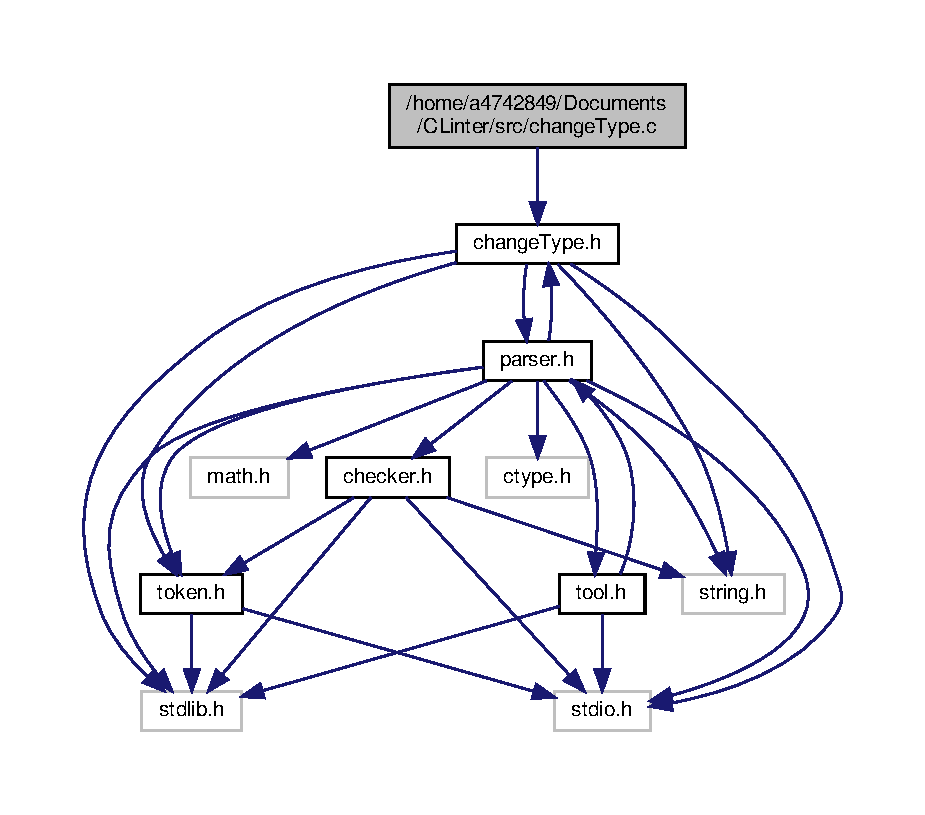
\includegraphics[width=350pt]{changeType_8c__incl}
\end{center}
\end{figure}
\subsection*{Functions}
\begin{DoxyCompactItemize}
\item 
void \hyperlink{changeType_8c_a2758f5a59b5f941678206601cdcd1d35}{assign\+Types} (\hyperlink{token_8h_af79b1a4f53ad41cc0de4b364b9455dba}{Token} $\ast$$\ast$list\+Token, int nb\+Nodes)
\begin{DoxyCompactList}\small\item\em Assign Types for a list of Tokens. \end{DoxyCompactList}\end{DoxyCompactItemize}


\subsection{Detailed Description}
This c file will contain all functions to change type of a token. 

\begin{DoxyAuthor}{Author}
Antoine T\+A\+V\+E\+R\+N\+I\+ER
\end{DoxyAuthor}
\begin{DoxyDate}{Date}
16/11/2018 
\end{DoxyDate}


\subsection{Function Documentation}
\mbox{\Hypertarget{changeType_8c_a2758f5a59b5f941678206601cdcd1d35}\label{changeType_8c_a2758f5a59b5f941678206601cdcd1d35}} 
\index{change\+Type.\+c@{change\+Type.\+c}!assign\+Types@{assign\+Types}}
\index{assign\+Types@{assign\+Types}!change\+Type.\+c@{change\+Type.\+c}}
\subsubsection{\texorpdfstring{assign\+Types()}{assignTypes()}}
{\footnotesize\ttfamily void assign\+Types (\begin{DoxyParamCaption}\item[{\hyperlink{token_8h_af79b1a4f53ad41cc0de4b364b9455dba}{Token} $\ast$$\ast$}]{list\+Token,  }\item[{int}]{nb\+Nodes }\end{DoxyParamCaption})}



Assign Types for a list of Tokens. 

Assign new types to tokens.


\begin{DoxyParams}{Parameters}
{\em list\+Token} & List of Tokens \\
\hline
{\em nb\+Nodes} & Number of Tokens \\
\hline
\end{DoxyParams}

\hypertarget{changeType_8h}{}\section{/home/a4742849/\+Documents/\+C\+Linter/src/change\+Type.h File Reference}
\label{changeType_8h}\index{/home/a4742849/\+Documents/\+C\+Linter/src/change\+Type.\+h@{/home/a4742849/\+Documents/\+C\+Linter/src/change\+Type.\+h}}


This header file will contain all required definitions and basic utilities functions to change type of a token.  


{\ttfamily \#include $<$stdlib.\+h$>$}\newline
{\ttfamily \#include $<$stdio.\+h$>$}\newline
{\ttfamily \#include $<$string.\+h$>$}\newline
{\ttfamily \#include \char`\"{}token.\+h\char`\"{}}\newline
{\ttfamily \#include \char`\"{}parser.\+h\char`\"{}}\newline
Include dependency graph for change\+Type.\+h\+:\nopagebreak
\begin{figure}[H]
\begin{center}
\leavevmode
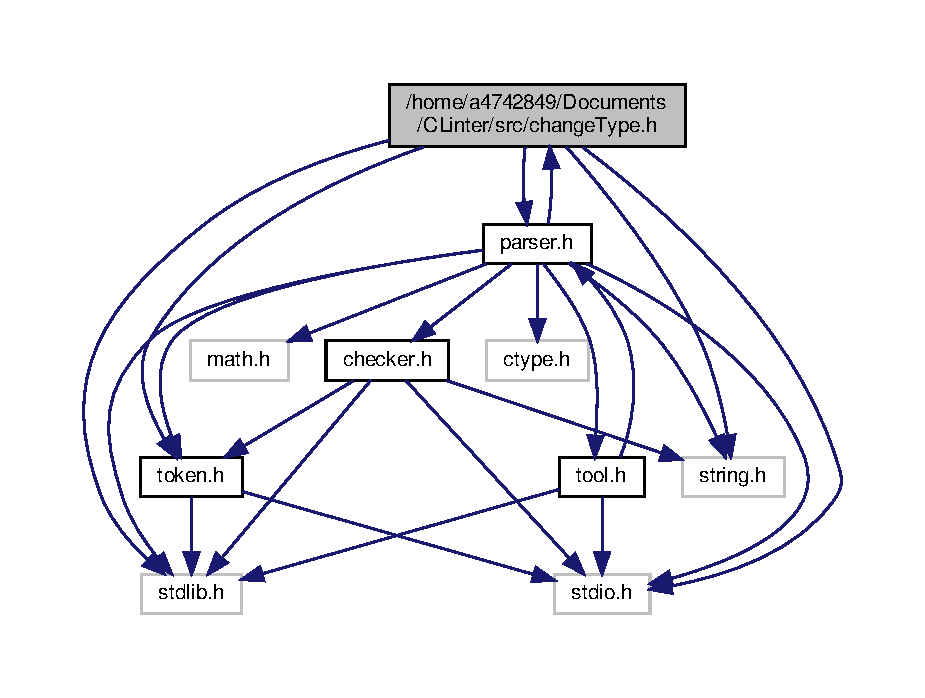
\includegraphics[width=350pt]{changeType_8h__incl}
\end{center}
\end{figure}
This graph shows which files directly or indirectly include this file\+:
\nopagebreak
\begin{figure}[H]
\begin{center}
\leavevmode
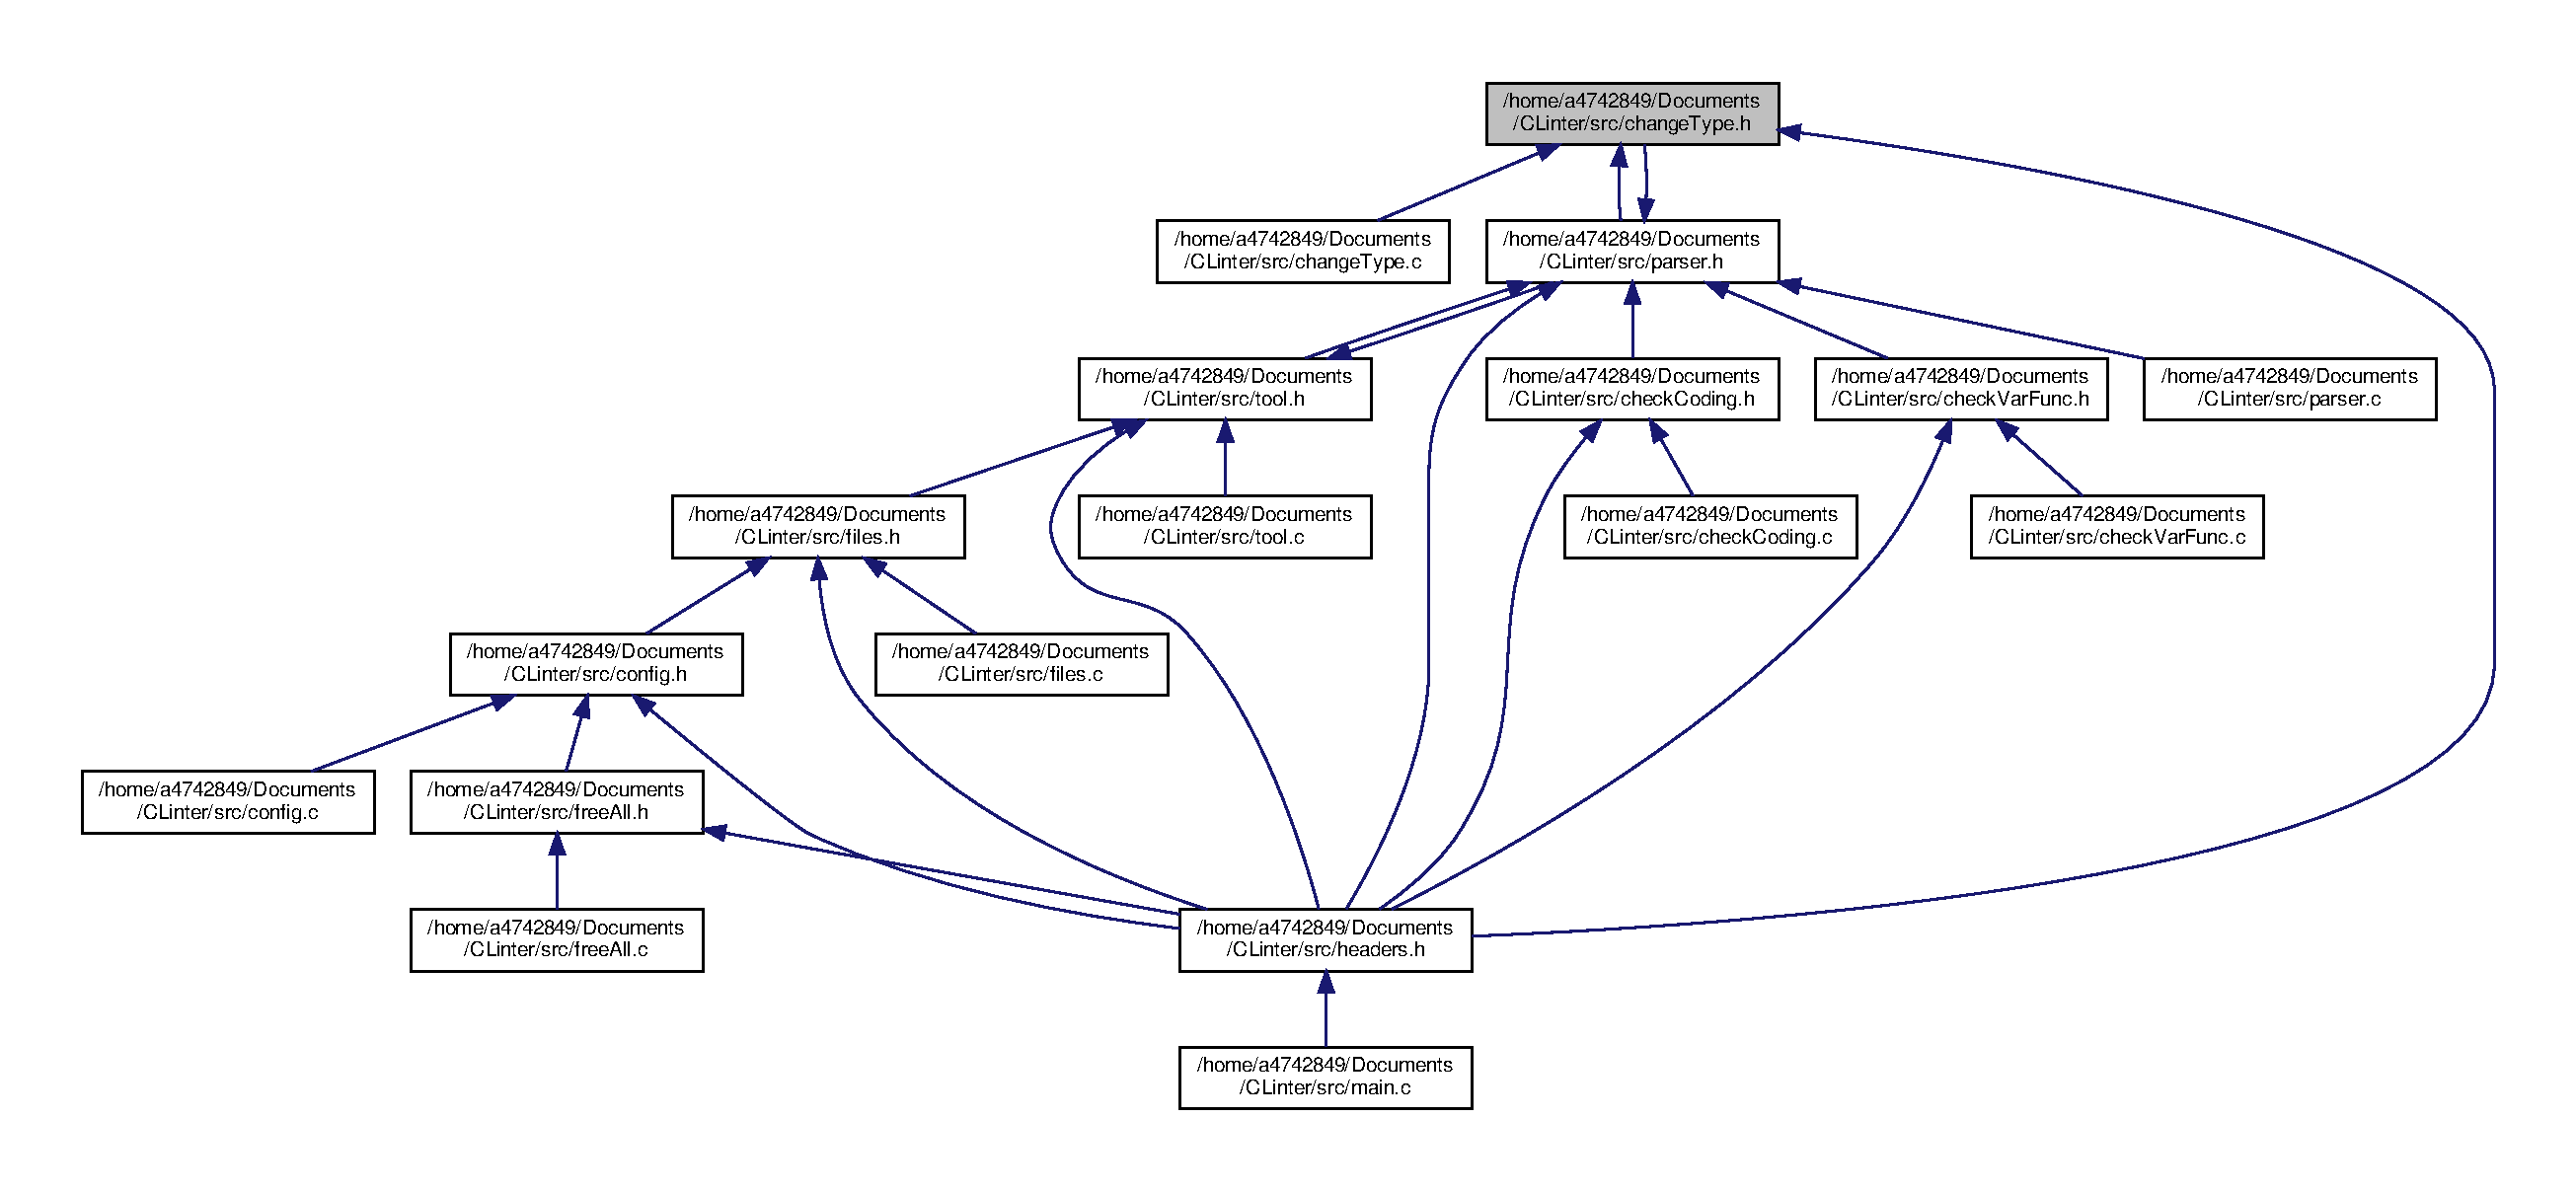
\includegraphics[width=350pt]{changeType_8h__dep__incl}
\end{center}
\end{figure}
\subsection*{Functions}
\begin{DoxyCompactItemize}
\item 
void \hyperlink{changeType_8h_a2758f5a59b5f941678206601cdcd1d35}{assign\+Types} (\hyperlink{token_8h_af79b1a4f53ad41cc0de4b364b9455dba}{Token} $\ast$$\ast$list\+Token, int nb\+Nodes)
\begin{DoxyCompactList}\small\item\em Assign new types to tokens. \end{DoxyCompactList}\end{DoxyCompactItemize}


\subsection{Detailed Description}
This header file will contain all required definitions and basic utilities functions to change type of a token. 

\begin{DoxyAuthor}{Author}
Antoine T\+A\+V\+E\+R\+N\+I\+ER
\end{DoxyAuthor}
\begin{DoxyDate}{Date}
16/11/2018 
\end{DoxyDate}


\subsection{Function Documentation}
\mbox{\Hypertarget{changeType_8h_a2758f5a59b5f941678206601cdcd1d35}\label{changeType_8h_a2758f5a59b5f941678206601cdcd1d35}} 
\index{change\+Type.\+h@{change\+Type.\+h}!assign\+Types@{assign\+Types}}
\index{assign\+Types@{assign\+Types}!change\+Type.\+h@{change\+Type.\+h}}
\subsubsection{\texorpdfstring{assign\+Types()}{assignTypes()}}
{\footnotesize\ttfamily void assign\+Types (\begin{DoxyParamCaption}\item[{\hyperlink{token_8h_af79b1a4f53ad41cc0de4b364b9455dba}{Token} $\ast$$\ast$}]{list\+Token,  }\item[{int}]{nb\+Nodes }\end{DoxyParamCaption})}



Assign new types to tokens. 


\begin{DoxyParams}{Parameters}
{\em list\+Token} & \\
\hline
{\em nb\+Nodes} & \\
\hline
\end{DoxyParams}
Assign new types to tokens.


\begin{DoxyParams}{Parameters}
{\em list\+Token} & List of Tokens \\
\hline
{\em nb\+Nodes} & Number of Tokens \\
\hline
\end{DoxyParams}

\hypertarget{checkCoding_8c}{}\section{/home/a4742849/\+Documents/\+C\+Linter/src/check\+Coding.c File Reference}
\label{checkCoding_8c}\index{/home/a4742849/\+Documents/\+C\+Linter/src/check\+Coding.\+c@{/home/a4742849/\+Documents/\+C\+Linter/src/check\+Coding.\+c}}


This c file will contain all functions to check simple coding style rules.  


{\ttfamily \#include \char`\"{}check\+Coding.\+h\char`\"{}}\newline
Include dependency graph for check\+Coding.\+c\+:\nopagebreak
\begin{figure}[H]
\begin{center}
\leavevmode
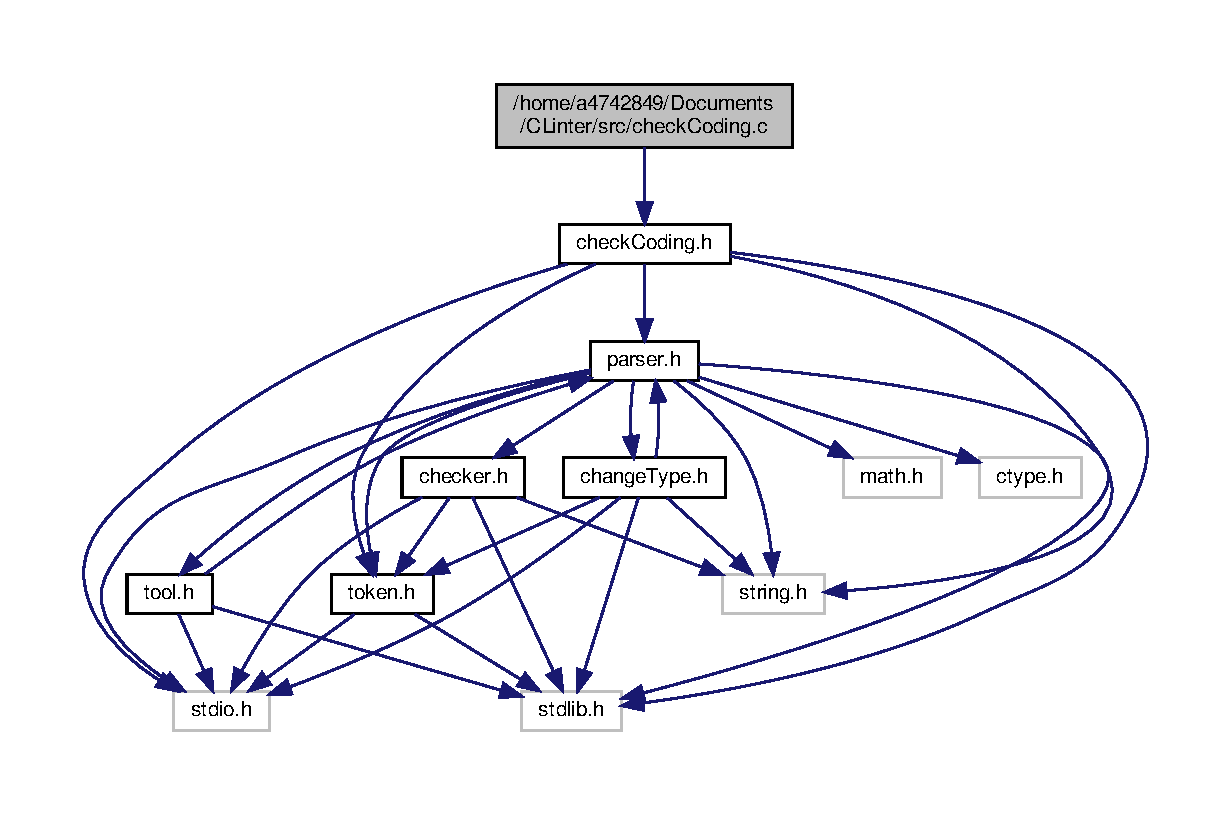
\includegraphics[width=350pt]{checkCoding_8c__incl}
\end{center}
\end{figure}
\subsection*{Functions}
\begin{DoxyCompactItemize}
\item 
void \hyperlink{checkCoding_8c_a970a5abd1aa70c5c011251a409bb7cef}{check\+Comments\+Header} (\hyperlink{token_8h_af79b1a4f53ad41cc0de4b364b9455dba}{Token} $\ast$$\ast$list\+Token, int nb\+Token, int line, char $\ast$file\+Name, int $\ast$status, int last\+Line)
\begin{DoxyCompactList}\small\item\em Check the rule comments-\/header. \end{DoxyCompactList}\item 
void \hyperlink{checkCoding_8c_a895b80e00435b977923e6c76b0e5e8a4}{checkmax\+Line\+Numbers} (int line, int nb\+Char, int max\+Line, char $\ast$file\+Name)
\begin{DoxyCompactList}\small\item\em max-\/line-\/numbers \end{DoxyCompactList}\item 
void \hyperlink{checkCoding_8c_a90875d0139aa266b01544d93104ec154}{checkmax\+File\+Line\+Numbers} (int nb\+Lines, int lines\+Conf, char $\ast$fil\+Name)
\item 
void \hyperlink{checkCoding_8c_aef74e3a94fd44ceeb0d9507b23377039}{check\+Operator} (\hyperlink{token_8h_af79b1a4f53ad41cc0de4b364b9455dba}{Token} $\ast$$\ast$list\+Token, int nb\+Token, int line, char $\ast$file\+Name)
\begin{DoxyCompactList}\small\item\em Check the rule operators-\/spacing. \end{DoxyCompactList}\item 
void \hyperlink{checkCoding_8c_a3d0c3d0ce365b355468e2deddfb921cb}{check\+Bracket} (\hyperlink{token_8h_af79b1a4f53ad41cc0de4b364b9455dba}{Token} $\ast$$\ast$list\+Token, int line, char $\ast$file\+Name)
\begin{DoxyCompactList}\small\item\em Check the rule array-\/bracket-\/eol. \end{DoxyCompactList}\item 
void \hyperlink{checkCoding_8c_a5211ee8ffa38f96f2d5655f1a0d61f34}{check\+Space} (\hyperlink{token_8h_af79b1a4f53ad41cc0de4b364b9455dba}{Token} $\ast$$\ast$list\+Token, int nb\+Token, int line, char $\ast$file\+Name)
\begin{DoxyCompactList}\small\item\em Check the rule no-\/trailing-\/spaces. \end{DoxyCompactList}\end{DoxyCompactItemize}


\subsection{Detailed Description}
This c file will contain all functions to check simple coding style rules. 

\begin{DoxyAuthor}{Author}
Antoine T\+A\+V\+E\+R\+N\+I\+ER
\end{DoxyAuthor}
\begin{DoxyDate}{Date}
16/11/2018 
\end{DoxyDate}


\subsection{Function Documentation}
\mbox{\Hypertarget{checkCoding_8c_a3d0c3d0ce365b355468e2deddfb921cb}\label{checkCoding_8c_a3d0c3d0ce365b355468e2deddfb921cb}} 
\index{check\+Coding.\+c@{check\+Coding.\+c}!check\+Bracket@{check\+Bracket}}
\index{check\+Bracket@{check\+Bracket}!check\+Coding.\+c@{check\+Coding.\+c}}
\subsubsection{\texorpdfstring{check\+Bracket()}{checkBracket()}}
{\footnotesize\ttfamily void check\+Bracket (\begin{DoxyParamCaption}\item[{\hyperlink{token_8h_af79b1a4f53ad41cc0de4b364b9455dba}{Token} $\ast$$\ast$}]{list\+Token,  }\item[{int}]{line,  }\item[{char $\ast$}]{file\+Name }\end{DoxyParamCaption})}



Check the rule array-\/bracket-\/eol. 


\begin{DoxyParams}{Parameters}
{\em list\+Token} & List of Tokens \\
\hline
{\em line} & Line in the file \\
\hline
{\em file\+Name} & File name we are working on \\
\hline
\end{DoxyParams}
\mbox{\Hypertarget{checkCoding_8c_a970a5abd1aa70c5c011251a409bb7cef}\label{checkCoding_8c_a970a5abd1aa70c5c011251a409bb7cef}} 
\index{check\+Coding.\+c@{check\+Coding.\+c}!check\+Comments\+Header@{check\+Comments\+Header}}
\index{check\+Comments\+Header@{check\+Comments\+Header}!check\+Coding.\+c@{check\+Coding.\+c}}
\subsubsection{\texorpdfstring{check\+Comments\+Header()}{checkCommentsHeader()}}
{\footnotesize\ttfamily void check\+Comments\+Header (\begin{DoxyParamCaption}\item[{\hyperlink{token_8h_af79b1a4f53ad41cc0de4b364b9455dba}{Token} $\ast$$\ast$}]{list\+Token,  }\item[{int}]{nb\+Token,  }\item[{int}]{line,  }\item[{char $\ast$}]{file\+Name,  }\item[{int $\ast$}]{status,  }\item[{int}]{last\+Line }\end{DoxyParamCaption})}



Check the rule comments-\/header. 


\begin{DoxyParams}{Parameters}
{\em list\+Token} & List of Tokens \\
\hline
{\em nb\+Token} & number of Tokens \\
\hline
{\em line} & Line in the file \\
\hline
{\em status} & State of comment header. 0 no comment. 1 Only opening Comment. 2 closed Comment \\
\hline
{\em last\+Line} & Helps to trigger the warning message at end of file \\
\hline
{\em file\+Name} & File name we are working on \\
\hline
\end{DoxyParams}
\mbox{\Hypertarget{checkCoding_8c_a90875d0139aa266b01544d93104ec154}\label{checkCoding_8c_a90875d0139aa266b01544d93104ec154}} 
\index{check\+Coding.\+c@{check\+Coding.\+c}!checkmax\+File\+Line\+Numbers@{checkmax\+File\+Line\+Numbers}}
\index{checkmax\+File\+Line\+Numbers@{checkmax\+File\+Line\+Numbers}!check\+Coding.\+c@{check\+Coding.\+c}}
\subsubsection{\texorpdfstring{checkmax\+File\+Line\+Numbers()}{checkmaxFileLineNumbers()}}
{\footnotesize\ttfamily void checkmax\+File\+Line\+Numbers (\begin{DoxyParamCaption}\item[{int}]{nb\+Lines,  }\item[{int}]{lines\+Conf,  }\item[{char $\ast$}]{fil\+Name }\end{DoxyParamCaption})}


\begin{DoxyParams}{Parameters}
{\em nb\+Lines} & Number of lines in the file \\
\hline
{\em lines\+Conf} & Number max of lines in a file from configuration \\
\hline
{\em fil\+Name} & File name we are working on \\
\hline
\end{DoxyParams}
\mbox{\Hypertarget{checkCoding_8c_a895b80e00435b977923e6c76b0e5e8a4}\label{checkCoding_8c_a895b80e00435b977923e6c76b0e5e8a4}} 
\index{check\+Coding.\+c@{check\+Coding.\+c}!checkmax\+Line\+Numbers@{checkmax\+Line\+Numbers}}
\index{checkmax\+Line\+Numbers@{checkmax\+Line\+Numbers}!check\+Coding.\+c@{check\+Coding.\+c}}
\subsubsection{\texorpdfstring{checkmax\+Line\+Numbers()}{checkmaxLineNumbers()}}
{\footnotesize\ttfamily void checkmax\+Line\+Numbers (\begin{DoxyParamCaption}\item[{int}]{line,  }\item[{int}]{nb\+Char,  }\item[{int}]{max\+Line,  }\item[{char $\ast$}]{file\+Name }\end{DoxyParamCaption})}



max-\/line-\/numbers 


\begin{DoxyParams}{Parameters}
{\em line} & Line in the file \\
\hline
{\em nb\+Char} & Number of character in the line \\
\hline
{\em max\+Line} & Number max of character in the line \\
\hline
{\em file\+Name} & File name we are working on \\
\hline
\end{DoxyParams}
\mbox{\Hypertarget{checkCoding_8c_aef74e3a94fd44ceeb0d9507b23377039}\label{checkCoding_8c_aef74e3a94fd44ceeb0d9507b23377039}} 
\index{check\+Coding.\+c@{check\+Coding.\+c}!check\+Operator@{check\+Operator}}
\index{check\+Operator@{check\+Operator}!check\+Coding.\+c@{check\+Coding.\+c}}
\subsubsection{\texorpdfstring{check\+Operator()}{checkOperator()}}
{\footnotesize\ttfamily void check\+Operator (\begin{DoxyParamCaption}\item[{\hyperlink{token_8h_af79b1a4f53ad41cc0de4b364b9455dba}{Token} $\ast$$\ast$}]{list\+Token,  }\item[{int}]{nb\+Token,  }\item[{int}]{line,  }\item[{char $\ast$}]{file\+Name }\end{DoxyParamCaption})}



Check the rule operators-\/spacing. 


\begin{DoxyParams}{Parameters}
{\em list\+Token} & List of Tokens \\
\hline
{\em nb\+Token} & number of Tokens \\
\hline
{\em line} & Line in the file \\
\hline
{\em file\+Name} & File name we are working on \\
\hline
\end{DoxyParams}
\mbox{\Hypertarget{checkCoding_8c_a5211ee8ffa38f96f2d5655f1a0d61f34}\label{checkCoding_8c_a5211ee8ffa38f96f2d5655f1a0d61f34}} 
\index{check\+Coding.\+c@{check\+Coding.\+c}!check\+Space@{check\+Space}}
\index{check\+Space@{check\+Space}!check\+Coding.\+c@{check\+Coding.\+c}}
\subsubsection{\texorpdfstring{check\+Space()}{checkSpace()}}
{\footnotesize\ttfamily void check\+Space (\begin{DoxyParamCaption}\item[{\hyperlink{token_8h_af79b1a4f53ad41cc0de4b364b9455dba}{Token} $\ast$$\ast$}]{list\+Token,  }\item[{int}]{nb\+Token,  }\item[{int}]{line,  }\item[{char $\ast$}]{file\+Name }\end{DoxyParamCaption})}



Check the rule no-\/trailing-\/spaces. 


\begin{DoxyParams}{Parameters}
{\em list\+Token} & List of Tokens \\
\hline
{\em nb\+Token} & number of Tokens \\
\hline
{\em line} & Line in the file \\
\hline
{\em file\+Name} & File name we are working on \\
\hline
\end{DoxyParams}

\hypertarget{checkCoding_8h}{}\section{/home/a4742849/\+Documents/\+C\+Linter/src/check\+Coding.h File Reference}
\label{checkCoding_8h}\index{/home/a4742849/\+Documents/\+C\+Linter/src/check\+Coding.\+h@{/home/a4742849/\+Documents/\+C\+Linter/src/check\+Coding.\+h}}


This header file will contain all required definitions and basic utilities functions to check rules on a C file.  


{\ttfamily \#include $<$stdlib.\+h$>$}\newline
{\ttfamily \#include $<$stdio.\+h$>$}\newline
{\ttfamily \#include $<$string.\+h$>$}\newline
{\ttfamily \#include \char`\"{}token.\+h\char`\"{}}\newline
{\ttfamily \#include \char`\"{}parser.\+h\char`\"{}}\newline
Include dependency graph for check\+Coding.\+h\+:\nopagebreak
\begin{figure}[H]
\begin{center}
\leavevmode
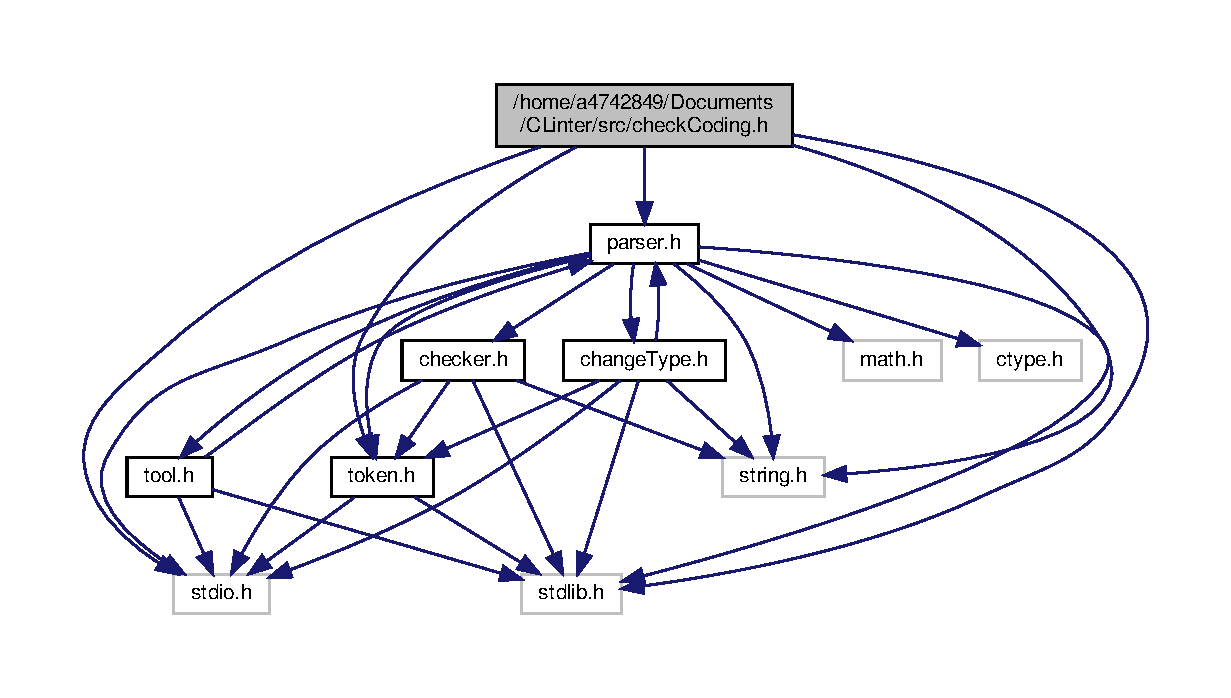
\includegraphics[width=350pt]{checkCoding_8h__incl}
\end{center}
\end{figure}
This graph shows which files directly or indirectly include this file\+:
\nopagebreak
\begin{figure}[H]
\begin{center}
\leavevmode
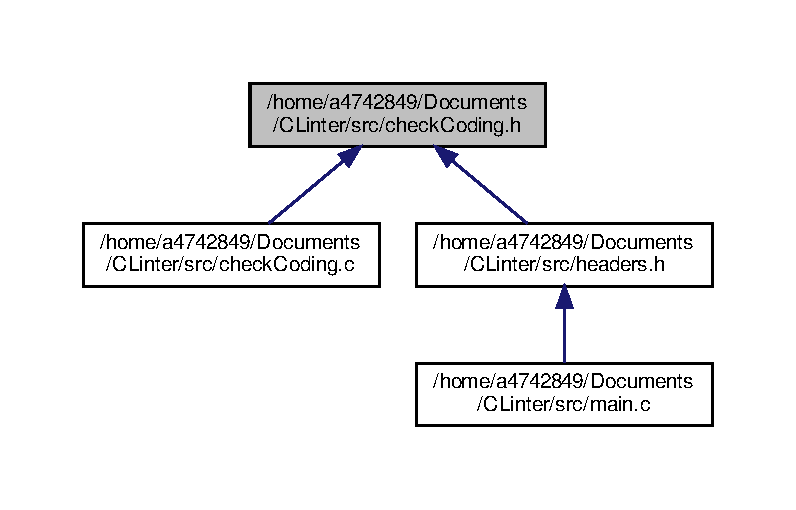
\includegraphics[width=350pt]{checkCoding_8h__dep__incl}
\end{center}
\end{figure}
\subsection*{Functions}
\begin{DoxyCompactItemize}
\item 
void \hyperlink{checkCoding_8h_a970a5abd1aa70c5c011251a409bb7cef}{check\+Comments\+Header} (\hyperlink{token_8h_af79b1a4f53ad41cc0de4b364b9455dba}{Token} $\ast$$\ast$list\+Token, int nb\+Token, int line, char $\ast$file\+Name, int $\ast$status, int last\+Line)
\begin{DoxyCompactList}\small\item\em Check the rule comments-\/header. \end{DoxyCompactList}\item 
void \hyperlink{checkCoding_8h_a895b80e00435b977923e6c76b0e5e8a4}{checkmax\+Line\+Numbers} (int line, int nb\+Char, int max\+Line, char $\ast$file\+Name)
\begin{DoxyCompactList}\small\item\em max-\/line-\/numbers \end{DoxyCompactList}\item 
void \hyperlink{checkCoding_8h_a8e9e839cbbd088458cb97acaee5d76f6}{checkmax\+File\+Line\+Numbers} (int nb\+Lines, int lines\+Conf, char $\ast$file\+Name)
\item 
void \hyperlink{checkCoding_8h_aef74e3a94fd44ceeb0d9507b23377039}{check\+Operator} (\hyperlink{token_8h_af79b1a4f53ad41cc0de4b364b9455dba}{Token} $\ast$$\ast$list\+Token, int nb\+Token, int line, char $\ast$file\+Name)
\begin{DoxyCompactList}\small\item\em Check the rule operators-\/spacing. \end{DoxyCompactList}\item 
void \hyperlink{checkCoding_8h_a5211ee8ffa38f96f2d5655f1a0d61f34}{check\+Space} (\hyperlink{token_8h_af79b1a4f53ad41cc0de4b364b9455dba}{Token} $\ast$$\ast$list\+Token, int nb\+Token, int line, char $\ast$file\+Name)
\begin{DoxyCompactList}\small\item\em Check the rule no-\/trailing-\/spaces. \end{DoxyCompactList}\item 
void \hyperlink{checkCoding_8h_a3d0c3d0ce365b355468e2deddfb921cb}{check\+Bracket} (\hyperlink{token_8h_af79b1a4f53ad41cc0de4b364b9455dba}{Token} $\ast$$\ast$list\+Token, int line, char $\ast$file\+Name)
\begin{DoxyCompactList}\small\item\em Check the rule array-\/bracket-\/eol. \end{DoxyCompactList}\end{DoxyCompactItemize}


\subsection{Detailed Description}
This header file will contain all required definitions and basic utilities functions to check rules on a C file. 

\begin{DoxyAuthor}{Author}
Antoine T\+A\+V\+E\+R\+N\+I\+ER
\end{DoxyAuthor}
\begin{DoxyDate}{Date}
16/11/2018 
\end{DoxyDate}


\subsection{Function Documentation}
\mbox{\Hypertarget{checkCoding_8h_a3d0c3d0ce365b355468e2deddfb921cb}\label{checkCoding_8h_a3d0c3d0ce365b355468e2deddfb921cb}} 
\index{check\+Coding.\+h@{check\+Coding.\+h}!check\+Bracket@{check\+Bracket}}
\index{check\+Bracket@{check\+Bracket}!check\+Coding.\+h@{check\+Coding.\+h}}
\subsubsection{\texorpdfstring{check\+Bracket()}{checkBracket()}}
{\footnotesize\ttfamily void check\+Bracket (\begin{DoxyParamCaption}\item[{\hyperlink{token_8h_af79b1a4f53ad41cc0de4b364b9455dba}{Token} $\ast$$\ast$}]{list\+Token,  }\item[{int}]{line,  }\item[{char $\ast$}]{file\+Name }\end{DoxyParamCaption})}



Check the rule array-\/bracket-\/eol. 


\begin{DoxyParams}{Parameters}
{\em list\+Token} & List of Tokens \\
\hline
{\em line} & Line in the file \\
\hline
{\em file\+Name} & File name we are working on \\
\hline
\end{DoxyParams}
\mbox{\Hypertarget{checkCoding_8h_a970a5abd1aa70c5c011251a409bb7cef}\label{checkCoding_8h_a970a5abd1aa70c5c011251a409bb7cef}} 
\index{check\+Coding.\+h@{check\+Coding.\+h}!check\+Comments\+Header@{check\+Comments\+Header}}
\index{check\+Comments\+Header@{check\+Comments\+Header}!check\+Coding.\+h@{check\+Coding.\+h}}
\subsubsection{\texorpdfstring{check\+Comments\+Header()}{checkCommentsHeader()}}
{\footnotesize\ttfamily void check\+Comments\+Header (\begin{DoxyParamCaption}\item[{\hyperlink{token_8h_af79b1a4f53ad41cc0de4b364b9455dba}{Token} $\ast$$\ast$}]{list\+Token,  }\item[{int}]{nb\+Token,  }\item[{int}]{line,  }\item[{char $\ast$}]{file\+Name,  }\item[{int $\ast$}]{status,  }\item[{int}]{last\+Line }\end{DoxyParamCaption})}



Check the rule comments-\/header. 


\begin{DoxyParams}{Parameters}
{\em list\+Token} & List of Tokens \\
\hline
{\em nb\+Token} & number of Tokens \\
\hline
{\em line} & Line in the file \\
\hline
{\em status} & State of comment header. 0 no comment. 1 Only opening Comment. 2 closed Comment \\
\hline
{\em last\+Line} & Helps to trigger the warning message at end of file \\
\hline
{\em file\+Name} & File name we are working on \\
\hline
\end{DoxyParams}
\mbox{\Hypertarget{checkCoding_8h_a8e9e839cbbd088458cb97acaee5d76f6}\label{checkCoding_8h_a8e9e839cbbd088458cb97acaee5d76f6}} 
\index{check\+Coding.\+h@{check\+Coding.\+h}!checkmax\+File\+Line\+Numbers@{checkmax\+File\+Line\+Numbers}}
\index{checkmax\+File\+Line\+Numbers@{checkmax\+File\+Line\+Numbers}!check\+Coding.\+h@{check\+Coding.\+h}}
\subsubsection{\texorpdfstring{checkmax\+File\+Line\+Numbers()}{checkmaxFileLineNumbers()}}
{\footnotesize\ttfamily void checkmax\+File\+Line\+Numbers (\begin{DoxyParamCaption}\item[{int}]{nb\+Lines,  }\item[{int}]{lines\+Conf,  }\item[{char $\ast$}]{fil\+Name }\end{DoxyParamCaption})}


\begin{DoxyParams}{Parameters}
{\em nb\+Lines} & Number of lines in the file \\
\hline
{\em lines\+Conf} & Number max of lines in a file from configuration \\
\hline
{\em fil\+Name} & File name we are working on \\
\hline
\end{DoxyParams}
\mbox{\Hypertarget{checkCoding_8h_a895b80e00435b977923e6c76b0e5e8a4}\label{checkCoding_8h_a895b80e00435b977923e6c76b0e5e8a4}} 
\index{check\+Coding.\+h@{check\+Coding.\+h}!checkmax\+Line\+Numbers@{checkmax\+Line\+Numbers}}
\index{checkmax\+Line\+Numbers@{checkmax\+Line\+Numbers}!check\+Coding.\+h@{check\+Coding.\+h}}
\subsubsection{\texorpdfstring{checkmax\+Line\+Numbers()}{checkmaxLineNumbers()}}
{\footnotesize\ttfamily void checkmax\+Line\+Numbers (\begin{DoxyParamCaption}\item[{int}]{line,  }\item[{int}]{nb\+Char,  }\item[{int}]{max\+Line,  }\item[{char $\ast$}]{file\+Name }\end{DoxyParamCaption})}



max-\/line-\/numbers 


\begin{DoxyParams}{Parameters}
{\em line} & Line in the file \\
\hline
{\em nb\+Char} & Number of character in the line \\
\hline
{\em max\+Line} & Number max of character in the line \\
\hline
{\em file\+Name} & File name we are working on \\
\hline
\end{DoxyParams}
\mbox{\Hypertarget{checkCoding_8h_aef74e3a94fd44ceeb0d9507b23377039}\label{checkCoding_8h_aef74e3a94fd44ceeb0d9507b23377039}} 
\index{check\+Coding.\+h@{check\+Coding.\+h}!check\+Operator@{check\+Operator}}
\index{check\+Operator@{check\+Operator}!check\+Coding.\+h@{check\+Coding.\+h}}
\subsubsection{\texorpdfstring{check\+Operator()}{checkOperator()}}
{\footnotesize\ttfamily void check\+Operator (\begin{DoxyParamCaption}\item[{\hyperlink{token_8h_af79b1a4f53ad41cc0de4b364b9455dba}{Token} $\ast$$\ast$}]{list\+Token,  }\item[{int}]{nb\+Token,  }\item[{int}]{line,  }\item[{char $\ast$}]{file\+Name }\end{DoxyParamCaption})}



Check the rule operators-\/spacing. 


\begin{DoxyParams}{Parameters}
{\em list\+Token} & List of Tokens \\
\hline
{\em nb\+Token} & number of Tokens \\
\hline
{\em line} & Line in the file \\
\hline
{\em file\+Name} & File name we are working on \\
\hline
\end{DoxyParams}
\mbox{\Hypertarget{checkCoding_8h_a5211ee8ffa38f96f2d5655f1a0d61f34}\label{checkCoding_8h_a5211ee8ffa38f96f2d5655f1a0d61f34}} 
\index{check\+Coding.\+h@{check\+Coding.\+h}!check\+Space@{check\+Space}}
\index{check\+Space@{check\+Space}!check\+Coding.\+h@{check\+Coding.\+h}}
\subsubsection{\texorpdfstring{check\+Space()}{checkSpace()}}
{\footnotesize\ttfamily void check\+Space (\begin{DoxyParamCaption}\item[{\hyperlink{token_8h_af79b1a4f53ad41cc0de4b364b9455dba}{Token} $\ast$$\ast$}]{list\+Token,  }\item[{int}]{nb\+Token,  }\item[{int}]{line,  }\item[{char $\ast$}]{file\+Name }\end{DoxyParamCaption})}



Check the rule no-\/trailing-\/spaces. 


\begin{DoxyParams}{Parameters}
{\em list\+Token} & List of Tokens \\
\hline
{\em nb\+Token} & number of Tokens \\
\hline
{\em line} & Line in the file \\
\hline
{\em file\+Name} & File name we are working on \\
\hline
\end{DoxyParams}

\hypertarget{checker_8c}{}\section{/home/a4742849/\+Documents/\+C\+Linter/src/checker.c File Reference}
\label{checker_8c}\index{/home/a4742849/\+Documents/\+C\+Linter/src/checker.\+c@{/home/a4742849/\+Documents/\+C\+Linter/src/checker.\+c}}


This c file will contain all functions to check a grammar.  


{\ttfamily \#include \char`\"{}checker.\+h\char`\"{}}\newline
Include dependency graph for checker.\+c\+:\nopagebreak
\begin{figure}[H]
\begin{center}
\leavevmode
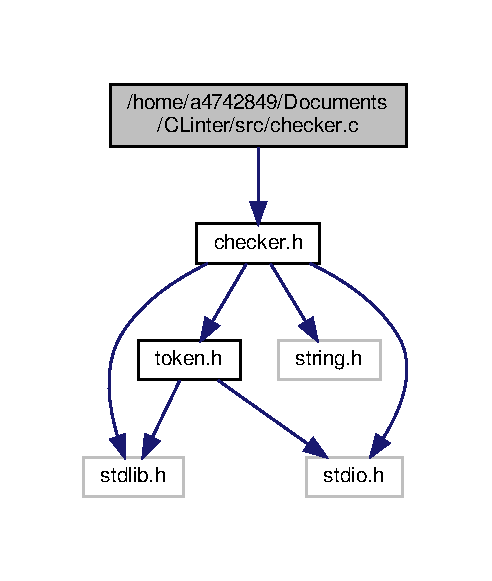
\includegraphics[width=236pt]{checker_8c__incl}
\end{center}
\end{figure}
\subsection*{Functions}
\begin{DoxyCompactItemize}
\item 
void \hyperlink{checker_8c_a84b143f5680c24af3bcd620ecee4e931}{print\+Err} (char $\ast$expected, char $\ast$found)
\begin{DoxyCompactList}\small\item\em Debug function to print Grammar errors. \end{DoxyCompactList}\item 
int \hyperlink{checker_8c_a4a0082e3143bf0a85f55ccfa37619b98}{match} (\hyperlink{token_8h_af79b1a4f53ad41cc0de4b364b9455dba}{Token} $\ast$tok, \hyperlink{token_8h_a16a6868f96564b3446a7f86b122b253e}{Type} type, char $\ast$val)
\begin{DoxyCompactList}\small\item\em Check if the Type matchs the type of the Token and the string content of the Token. \end{DoxyCompactList}\item 
void \hyperlink{checker_8c_a340149104df3bcabd21e3114ef9ac7b5}{next\+Tok} (int $\ast$pos, int nb\+Node, \hyperlink{token_8h_af79b1a4f53ad41cc0de4b364b9455dba}{Token} $\ast$$\ast$tokens)
\begin{DoxyCompactList}\small\item\em Updates the position value. \end{DoxyCompactList}\item 
int \hyperlink{checker_8c_adde228c5e9e66958fe2e6af41235f71e}{eat\+Token} (\hyperlink{token_8h_af79b1a4f53ad41cc0de4b364b9455dba}{Token} $\ast$$\ast$tokens, \hyperlink{token_8h_a16a6868f96564b3446a7f86b122b253e}{Type} type, int $\ast$pos, int nb\+Node)
\begin{DoxyCompactList}\small\item\em Tries to go to the next Token. \end{DoxyCompactList}\item 
void \hyperlink{checker_8c_ac036563d82d1d28457c1baa8dbdc5faa}{var\+Declare} (\hyperlink{token_8h_af79b1a4f53ad41cc0de4b364b9455dba}{Token} $\ast$$\ast$tokens, int $\ast$pos, int nb\+Node)
\begin{DoxyCompactList}\small\item\em Variables Declaration checker. \end{DoxyCompactList}\item 
void \hyperlink{checker_8c_ac6e030b30b03379f03101651ad86340b}{check} (\hyperlink{token_8h_af79b1a4f53ad41cc0de4b364b9455dba}{Token} $\ast$$\ast$tokens, int nb\+Node)
\begin{DoxyCompactList}\small\item\em Checks a specific Grammar, not used at the moment. \end{DoxyCompactList}\end{DoxyCompactItemize}


\subsection{Detailed Description}
This c file will contain all functions to check a grammar. 

\begin{DoxyAuthor}{Author}
Antoine T\+A\+V\+E\+R\+N\+I\+ER
\end{DoxyAuthor}
\begin{DoxyDate}{Date}
16/11/2018 
\end{DoxyDate}


\subsection{Function Documentation}
\mbox{\Hypertarget{checker_8c_ac6e030b30b03379f03101651ad86340b}\label{checker_8c_ac6e030b30b03379f03101651ad86340b}} 
\index{checker.\+c@{checker.\+c}!check@{check}}
\index{check@{check}!checker.\+c@{checker.\+c}}
\subsubsection{\texorpdfstring{check()}{check()}}
{\footnotesize\ttfamily void check (\begin{DoxyParamCaption}\item[{\hyperlink{token_8h_af79b1a4f53ad41cc0de4b364b9455dba}{Token} $\ast$$\ast$}]{tokens,  }\item[{int}]{nb\+Node }\end{DoxyParamCaption})}



Checks a specific Grammar, not used at the moment. 


\begin{DoxyParams}{Parameters}
{\em tokens} & List of Tokens \\
\hline
{\em nb\+Node} & Number of nodes \\
\hline
\end{DoxyParams}
\mbox{\Hypertarget{checker_8c_adde228c5e9e66958fe2e6af41235f71e}\label{checker_8c_adde228c5e9e66958fe2e6af41235f71e}} 
\index{checker.\+c@{checker.\+c}!eat\+Token@{eat\+Token}}
\index{eat\+Token@{eat\+Token}!checker.\+c@{checker.\+c}}
\subsubsection{\texorpdfstring{eat\+Token()}{eatToken()}}
{\footnotesize\ttfamily int eat\+Token (\begin{DoxyParamCaption}\item[{\hyperlink{token_8h_af79b1a4f53ad41cc0de4b364b9455dba}{Token} $\ast$$\ast$}]{tokens,  }\item[{\hyperlink{token_8h_a16a6868f96564b3446a7f86b122b253e}{Type}}]{type,  }\item[{int $\ast$}]{pos,  }\item[{int}]{nb\+Node }\end{DoxyParamCaption})}



Tries to go to the next Token. 


\begin{DoxyParams}{Parameters}
{\em tokens} & List of Tokens \\
\hline
{\em type} & Type of the expected Token \\
\hline
{\em pos} & Position in the list of Tokens \\
\hline
{\em nb\+Node} & Number of tokens in the list \\
\hline
\end{DoxyParams}
\begin{DoxyReturn}{Returns}
int 0 false else true 
\end{DoxyReturn}
\mbox{\Hypertarget{checker_8c_a4a0082e3143bf0a85f55ccfa37619b98}\label{checker_8c_a4a0082e3143bf0a85f55ccfa37619b98}} 
\index{checker.\+c@{checker.\+c}!match@{match}}
\index{match@{match}!checker.\+c@{checker.\+c}}
\subsubsection{\texorpdfstring{match()}{match()}}
{\footnotesize\ttfamily int match (\begin{DoxyParamCaption}\item[{\hyperlink{token_8h_af79b1a4f53ad41cc0de4b364b9455dba}{Token} $\ast$}]{tok,  }\item[{\hyperlink{token_8h_a16a6868f96564b3446a7f86b122b253e}{Type}}]{type,  }\item[{char $\ast$}]{val }\end{DoxyParamCaption})}



Check if the Type matchs the type of the Token and the string content of the Token. 


\begin{DoxyParams}{Parameters}
{\em tok} & Specific Token \\
\hline
{\em type} & Wanted Type to check \\
\hline
{\em val} & String to check \\
\hline
\end{DoxyParams}
\begin{DoxyReturn}{Returns}
int 0 false else true 
\end{DoxyReturn}
\mbox{\Hypertarget{checker_8c_a340149104df3bcabd21e3114ef9ac7b5}\label{checker_8c_a340149104df3bcabd21e3114ef9ac7b5}} 
\index{checker.\+c@{checker.\+c}!next\+Tok@{next\+Tok}}
\index{next\+Tok@{next\+Tok}!checker.\+c@{checker.\+c}}
\subsubsection{\texorpdfstring{next\+Tok()}{nextTok()}}
{\footnotesize\ttfamily void next\+Tok (\begin{DoxyParamCaption}\item[{int $\ast$}]{pos,  }\item[{int}]{nb\+Node,  }\item[{\hyperlink{token_8h_af79b1a4f53ad41cc0de4b364b9455dba}{Token} $\ast$$\ast$}]{tokens }\end{DoxyParamCaption})}



Updates the position value. 


\begin{DoxyParams}{Parameters}
{\em pos} & Position in the list of Tokens \\
\hline
{\em nb\+Node} & Number of tokens in the list of Tokens \\
\hline
{\em tokens} & List of Tokens \\
\hline
\end{DoxyParams}
\mbox{\Hypertarget{checker_8c_a84b143f5680c24af3bcd620ecee4e931}\label{checker_8c_a84b143f5680c24af3bcd620ecee4e931}} 
\index{checker.\+c@{checker.\+c}!print\+Err@{print\+Err}}
\index{print\+Err@{print\+Err}!checker.\+c@{checker.\+c}}
\subsubsection{\texorpdfstring{print\+Err()}{printErr()}}
{\footnotesize\ttfamily void print\+Err (\begin{DoxyParamCaption}\item[{char $\ast$}]{expected,  }\item[{char $\ast$}]{found }\end{DoxyParamCaption})}



Debug function to print Grammar errors. 


\begin{DoxyParams}{Parameters}
{\em expected} & String expected \\
\hline
{\em found} & String found \\
\hline
\end{DoxyParams}
\mbox{\Hypertarget{checker_8c_ac036563d82d1d28457c1baa8dbdc5faa}\label{checker_8c_ac036563d82d1d28457c1baa8dbdc5faa}} 
\index{checker.\+c@{checker.\+c}!var\+Declare@{var\+Declare}}
\index{var\+Declare@{var\+Declare}!checker.\+c@{checker.\+c}}
\subsubsection{\texorpdfstring{var\+Declare()}{varDeclare()}}
{\footnotesize\ttfamily void var\+Declare (\begin{DoxyParamCaption}\item[{\hyperlink{token_8h_af79b1a4f53ad41cc0de4b364b9455dba}{Token} $\ast$$\ast$}]{tokens,  }\item[{int $\ast$}]{pos,  }\item[{int}]{nb\+Node }\end{DoxyParamCaption})}



Variables Declaration checker. 


\begin{DoxyParams}{Parameters}
{\em tokens} & List of Tokens \\
\hline
{\em pos} & Position in the list of Tokens \\
\hline
{\em nb\+Node} & Number of tokens in the list \\
\hline
\end{DoxyParams}

\hypertarget{checker_8h}{}\section{/home/a4742849/\+Documents/\+C\+Linter/src/checker.h File Reference}
\label{checker_8h}\index{/home/a4742849/\+Documents/\+C\+Linter/src/checker.\+h@{/home/a4742849/\+Documents/\+C\+Linter/src/checker.\+h}}


This header file will contain all required definitions and basic utilities functions to check grammar of a C file.  


{\ttfamily \#include $<$stdlib.\+h$>$}\newline
{\ttfamily \#include $<$stdio.\+h$>$}\newline
{\ttfamily \#include $<$string.\+h$>$}\newline
{\ttfamily \#include \char`\"{}token.\+h\char`\"{}}\newline
Include dependency graph for checker.\+h\+:\nopagebreak
\begin{figure}[H]
\begin{center}
\leavevmode
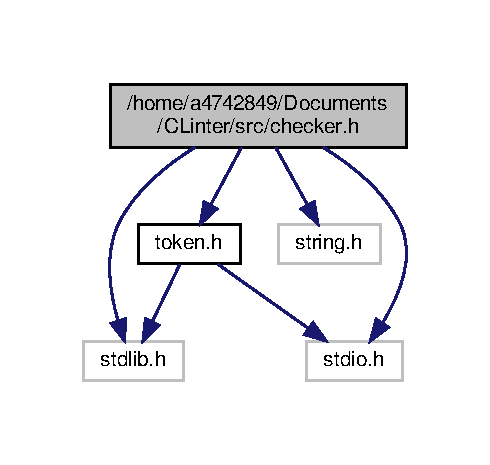
\includegraphics[width=235pt]{checker_8h__incl}
\end{center}
\end{figure}
This graph shows which files directly or indirectly include this file\+:
\nopagebreak
\begin{figure}[H]
\begin{center}
\leavevmode
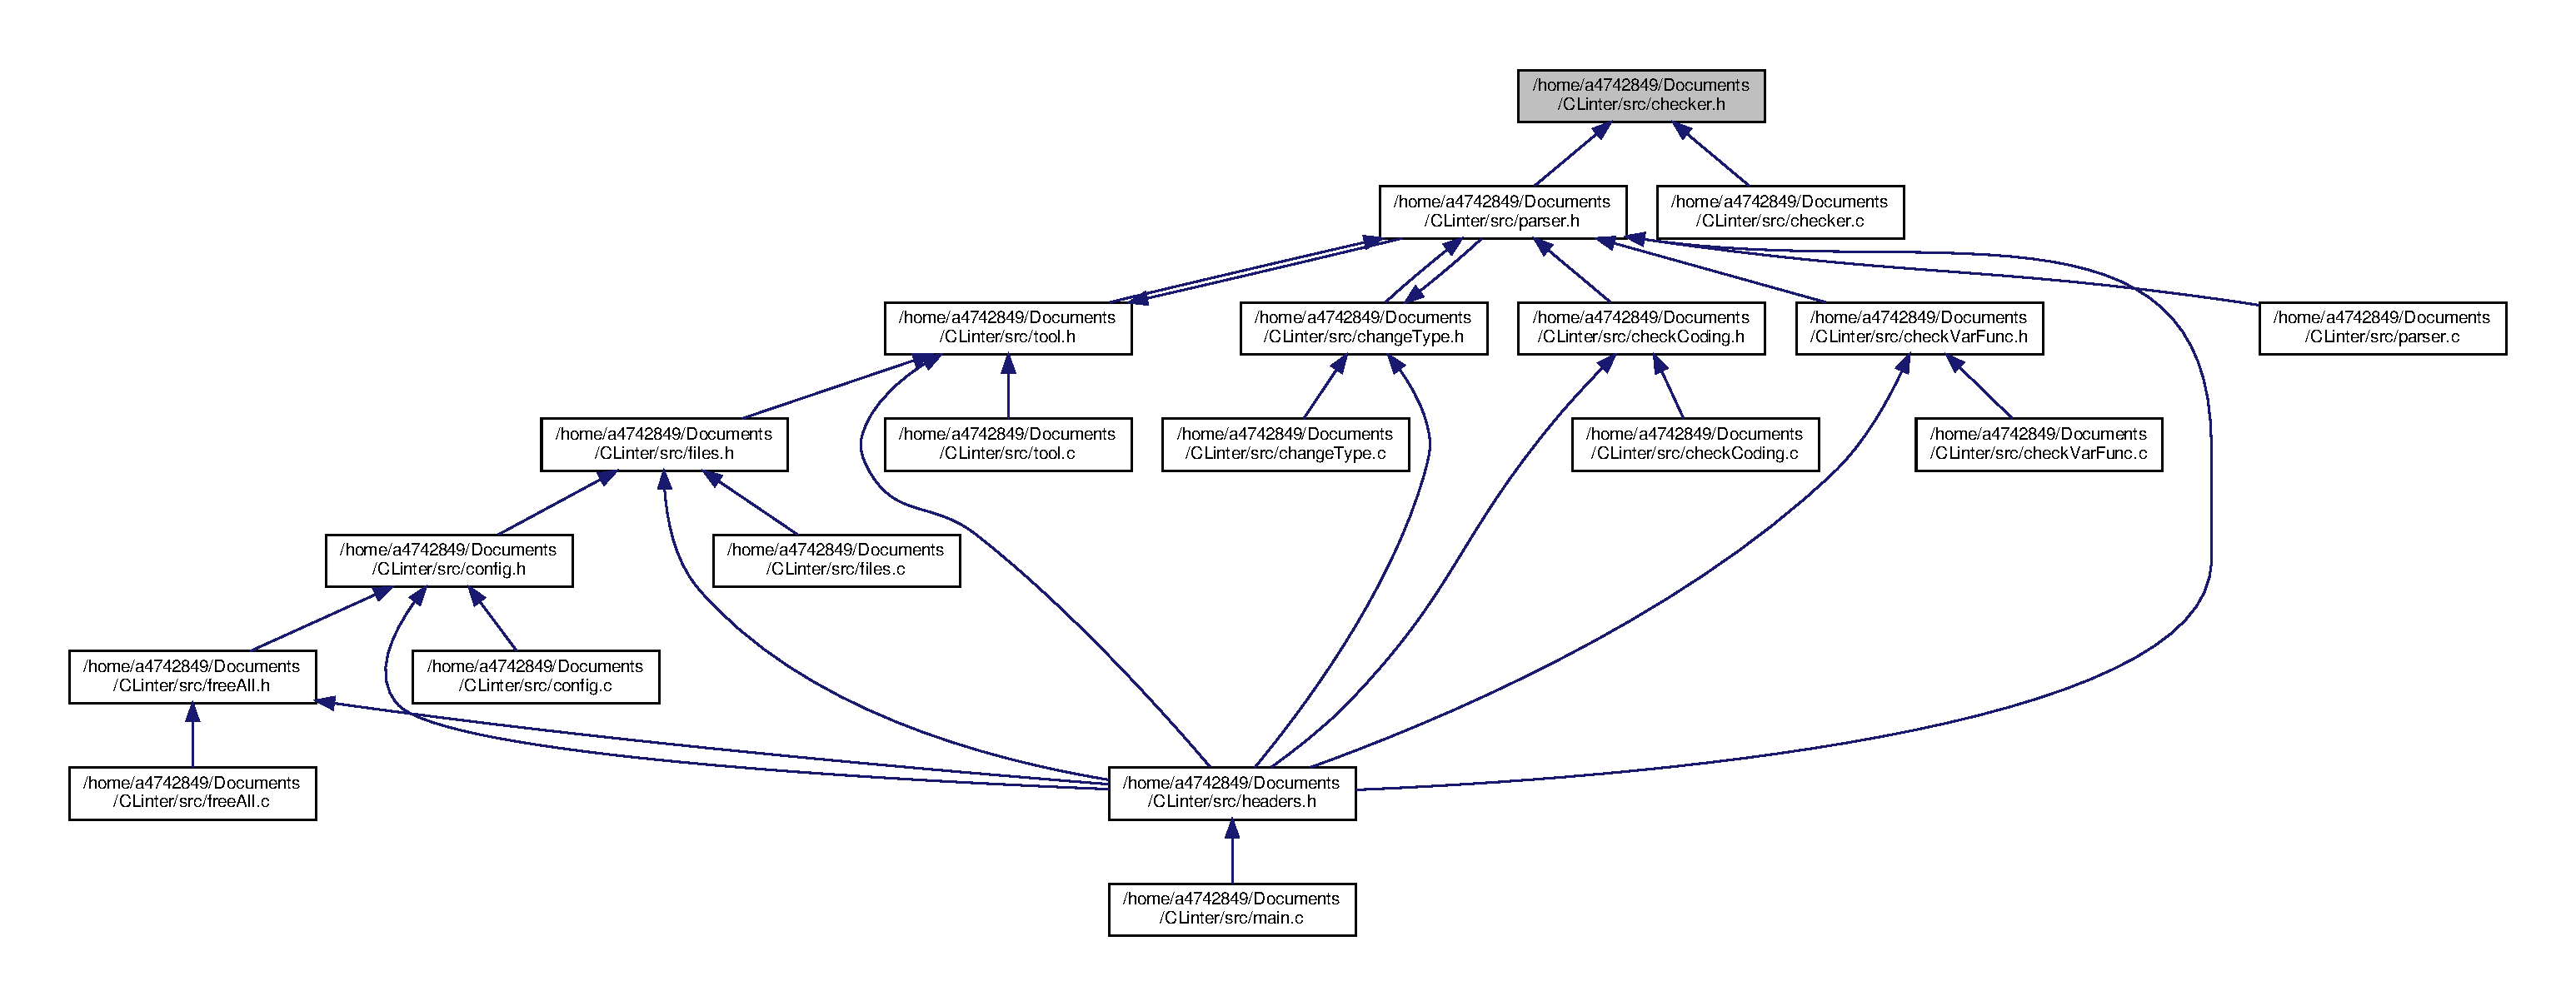
\includegraphics[width=350pt]{checker_8h__dep__incl}
\end{center}
\end{figure}
\subsection*{Functions}
\begin{DoxyCompactItemize}
\item 
void \hyperlink{checker_8h_af859dc84cfd7ba30c0032d993d0b5dc6}{check} (\hyperlink{token_8h_af79b1a4f53ad41cc0de4b364b9455dba}{Token} $\ast$$\ast$list\+Token, int nb\+Token)
\begin{DoxyCompactList}\small\item\em Checks a specific Grammar, not used at the moment. \end{DoxyCompactList}\end{DoxyCompactItemize}


\subsection{Detailed Description}
This header file will contain all required definitions and basic utilities functions to check grammar of a C file. 

\begin{DoxyAuthor}{Author}
Antoine T\+A\+V\+E\+R\+N\+I\+ER
\end{DoxyAuthor}
\begin{DoxyDate}{Date}
16/11/2018 
\end{DoxyDate}


\subsection{Function Documentation}
\mbox{\Hypertarget{checker_8h_af859dc84cfd7ba30c0032d993d0b5dc6}\label{checker_8h_af859dc84cfd7ba30c0032d993d0b5dc6}} 
\index{checker.\+h@{checker.\+h}!check@{check}}
\index{check@{check}!checker.\+h@{checker.\+h}}
\subsubsection{\texorpdfstring{check()}{check()}}
{\footnotesize\ttfamily void check (\begin{DoxyParamCaption}\item[{\hyperlink{token_8h_af79b1a4f53ad41cc0de4b364b9455dba}{Token} $\ast$$\ast$}]{tokens,  }\item[{int}]{nb\+Node }\end{DoxyParamCaption})}



Checks a specific Grammar, not used at the moment. 


\begin{DoxyParams}{Parameters}
{\em tokens} & List of Tokens \\
\hline
{\em nb\+Node} & Number of nodes \\
\hline
\end{DoxyParams}

\hypertarget{checkVarFunc_8c}{}\section{/home/a4742849/\+Documents/\+C\+Linter/src/check\+Var\+Func.c File Reference}
\label{checkVarFunc_8c}\index{/home/a4742849/\+Documents/\+C\+Linter/src/check\+Var\+Func.\+c@{/home/a4742849/\+Documents/\+C\+Linter/src/check\+Var\+Func.\+c}}


This c file will contain all functions to check rules on functions or variables.  


{\ttfamily \#include \char`\"{}check\+Var\+Func.\+h\char`\"{}}\newline
Include dependency graph for check\+Var\+Func.\+c\+:\nopagebreak
\begin{figure}[H]
\begin{center}
\leavevmode
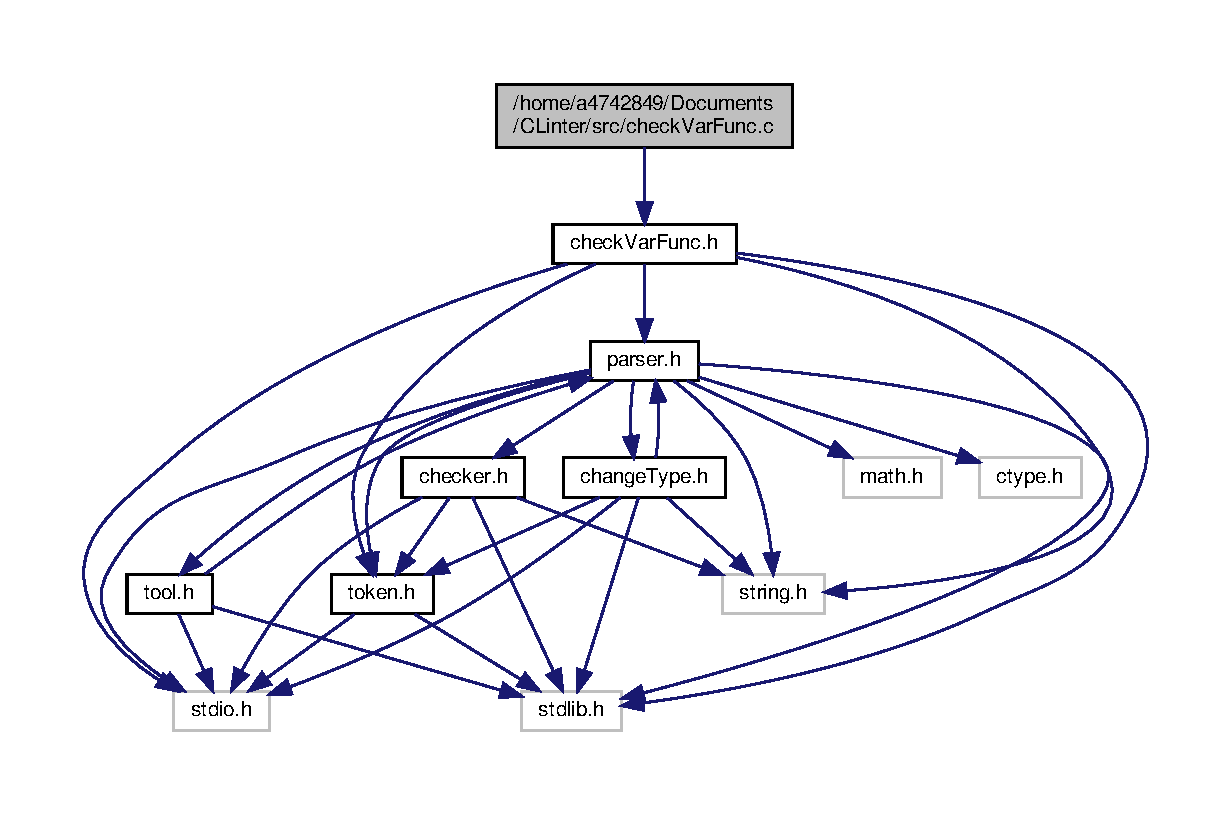
\includegraphics[width=350pt]{checkVarFunc_8c__incl}
\end{center}
\end{figure}
\subsection*{Functions}
\begin{DoxyCompactItemize}
\item 
int \hyperlink{checkVarFunc_8c_ad861d92c3af78a3167a2a74f3842a45d}{skip\+Spaces} (\hyperlink{token_8h_af79b1a4f53ad41cc0de4b364b9455dba}{Token} $\ast$$\ast$list\+Token, int nb\+Token)
\begin{DoxyCompactList}\small\item\em Skips the tokens with Delimiter Type. \end{DoxyCompactList}\item 
int \hyperlink{checkVarFunc_8c_a193af1a8315f360dd2ca04eac52b8a68}{contains\+Str} (\hyperlink{token_8h_af79b1a4f53ad41cc0de4b364b9455dba}{Token} $\ast$$\ast$list\+Token, int nb\+Token, char $\ast$str)
\begin{DoxyCompactList}\small\item\em Check if the list of Tokens contains a specific strins. \end{DoxyCompactList}\item 
void \hyperlink{checkVarFunc_8c_aac96c45baf06eeead031b0595f4af35f}{multi\+Declare} (\hyperlink{token_8h_af79b1a4f53ad41cc0de4b364b9455dba}{Token} $\ast$$\ast$list\+Token, int nb\+Token, int line, char $\ast$file\+Name)
\begin{DoxyCompactList}\small\item\em Check the rule multi declaration. \end{DoxyCompactList}\end{DoxyCompactItemize}


\subsection{Detailed Description}
This c file will contain all functions to check rules on functions or variables. 

\begin{DoxyAuthor}{Author}
Antoine T\+A\+V\+E\+R\+N\+I\+ER
\end{DoxyAuthor}
\begin{DoxyDate}{Date}
16/11/2018 
\end{DoxyDate}


\subsection{Function Documentation}
\mbox{\Hypertarget{checkVarFunc_8c_a193af1a8315f360dd2ca04eac52b8a68}\label{checkVarFunc_8c_a193af1a8315f360dd2ca04eac52b8a68}} 
\index{check\+Var\+Func.\+c@{check\+Var\+Func.\+c}!contains\+Str@{contains\+Str}}
\index{contains\+Str@{contains\+Str}!check\+Var\+Func.\+c@{check\+Var\+Func.\+c}}
\subsubsection{\texorpdfstring{contains\+Str()}{containsStr()}}
{\footnotesize\ttfamily int contains\+Str (\begin{DoxyParamCaption}\item[{\hyperlink{token_8h_af79b1a4f53ad41cc0de4b364b9455dba}{Token} $\ast$$\ast$}]{list\+Token,  }\item[{int}]{nb\+Token,  }\item[{char $\ast$}]{str }\end{DoxyParamCaption})}



Check if the list of Tokens contains a specific strins. 


\begin{DoxyParams}{Parameters}
{\em list\+Token} & List of Tokens \\
\hline
{\em nb\+Token} & Numbers of Tokens \\
\hline
{\em str} & String to check \\
\hline
\end{DoxyParams}
\begin{DoxyReturn}{Returns}
int 0 false else true 
\end{DoxyReturn}
\mbox{\Hypertarget{checkVarFunc_8c_aac96c45baf06eeead031b0595f4af35f}\label{checkVarFunc_8c_aac96c45baf06eeead031b0595f4af35f}} 
\index{check\+Var\+Func.\+c@{check\+Var\+Func.\+c}!multi\+Declare@{multi\+Declare}}
\index{multi\+Declare@{multi\+Declare}!check\+Var\+Func.\+c@{check\+Var\+Func.\+c}}
\subsubsection{\texorpdfstring{multi\+Declare()}{multiDeclare()}}
{\footnotesize\ttfamily void multi\+Declare (\begin{DoxyParamCaption}\item[{\hyperlink{token_8h_af79b1a4f53ad41cc0de4b364b9455dba}{Token} $\ast$$\ast$}]{list\+Token,  }\item[{int}]{nb\+Token,  }\item[{int}]{line,  }\item[{char $\ast$}]{file\+Name }\end{DoxyParamCaption})}



Check the rule multi declaration. 


\begin{DoxyParams}{Parameters}
{\em list\+Token} & List of Tokens \\
\hline
{\em nb\+Token} & Number of Tokens \\
\hline
{\em line} & At which line we are in the File \\
\hline
{\em file\+Name} & The file name \\
\hline
\end{DoxyParams}
\mbox{\Hypertarget{checkVarFunc_8c_ad861d92c3af78a3167a2a74f3842a45d}\label{checkVarFunc_8c_ad861d92c3af78a3167a2a74f3842a45d}} 
\index{check\+Var\+Func.\+c@{check\+Var\+Func.\+c}!skip\+Spaces@{skip\+Spaces}}
\index{skip\+Spaces@{skip\+Spaces}!check\+Var\+Func.\+c@{check\+Var\+Func.\+c}}
\subsubsection{\texorpdfstring{skip\+Spaces()}{skipSpaces()}}
{\footnotesize\ttfamily int skip\+Spaces (\begin{DoxyParamCaption}\item[{\hyperlink{token_8h_af79b1a4f53ad41cc0de4b364b9455dba}{Token} $\ast$$\ast$}]{list\+Token,  }\item[{int}]{nb\+Token }\end{DoxyParamCaption})}



Skips the tokens with Delimiter Type. 


\begin{DoxyParams}{Parameters}
{\em list\+Token} & List of Tokens \\
\hline
{\em nb\+Token} & Number of Tokens \\
\hline
\end{DoxyParams}
\begin{DoxyReturn}{Returns}
int 0 false else true 
\end{DoxyReturn}

\hypertarget{checkVarFunc_8h}{}\section{/home/a4742849/\+Documents/\+C\+Linter/src/check\+Var\+Func.h File Reference}
\label{checkVarFunc_8h}\index{/home/a4742849/\+Documents/\+C\+Linter/src/check\+Var\+Func.\+h@{/home/a4742849/\+Documents/\+C\+Linter/src/check\+Var\+Func.\+h}}


This header file will contain all required definitions and basic utilities functions to check rules on functions or variables on a C file.  


{\ttfamily \#include $<$stdlib.\+h$>$}\newline
{\ttfamily \#include $<$stdio.\+h$>$}\newline
{\ttfamily \#include $<$string.\+h$>$}\newline
{\ttfamily \#include \char`\"{}token.\+h\char`\"{}}\newline
{\ttfamily \#include \char`\"{}parser.\+h\char`\"{}}\newline
Include dependency graph for check\+Var\+Func.\+h\+:\nopagebreak
\begin{figure}[H]
\begin{center}
\leavevmode
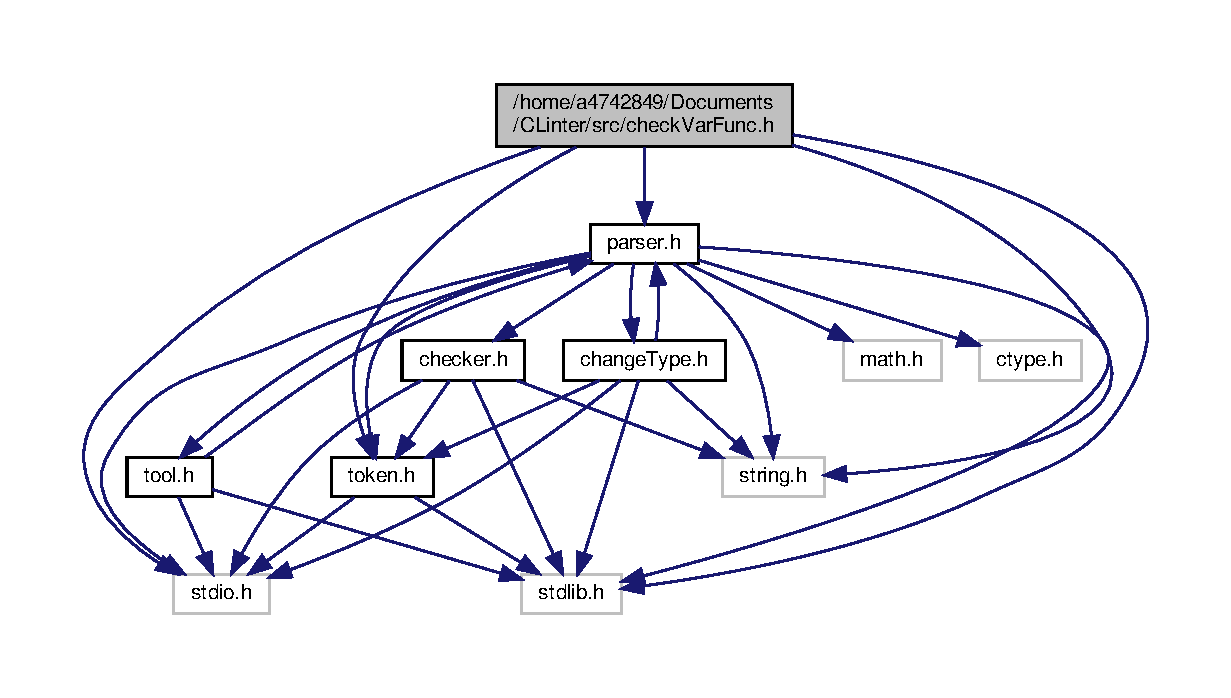
\includegraphics[width=350pt]{checkVarFunc_8h__incl}
\end{center}
\end{figure}
This graph shows which files directly or indirectly include this file\+:
\nopagebreak
\begin{figure}[H]
\begin{center}
\leavevmode
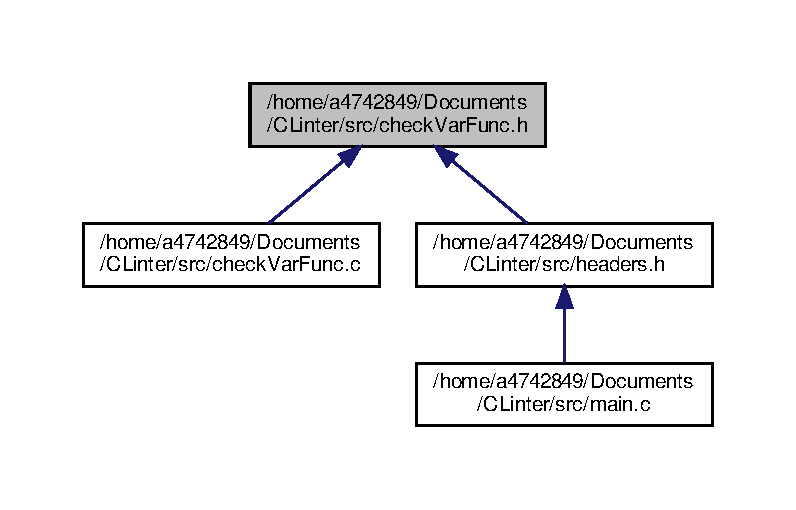
\includegraphics[width=350pt]{checkVarFunc_8h__dep__incl}
\end{center}
\end{figure}
\subsection*{Functions}
\begin{DoxyCompactItemize}
\item 
int \hyperlink{checkVarFunc_8h_ad861d92c3af78a3167a2a74f3842a45d}{skip\+Spaces} (\hyperlink{token_8h_af79b1a4f53ad41cc0de4b364b9455dba}{Token} $\ast$$\ast$list\+Token, int nb\+Token)
\begin{DoxyCompactList}\small\item\em Skips the tokens with Delimiter Type. \end{DoxyCompactList}\item 
int \hyperlink{checkVarFunc_8h_a193af1a8315f360dd2ca04eac52b8a68}{contains\+Str} (\hyperlink{token_8h_af79b1a4f53ad41cc0de4b364b9455dba}{Token} $\ast$$\ast$list\+Token, int nb\+Token, char $\ast$str)
\begin{DoxyCompactList}\small\item\em Check if the list of Tokens contains a specific strins. \end{DoxyCompactList}\item 
void \hyperlink{checkVarFunc_8h_aac96c45baf06eeead031b0595f4af35f}{multi\+Declare} (\hyperlink{token_8h_af79b1a4f53ad41cc0de4b364b9455dba}{Token} $\ast$$\ast$list\+Token, int nb\+Token, int line, char $\ast$file\+Name)
\begin{DoxyCompactList}\small\item\em Check the rule multi declaration. \end{DoxyCompactList}\end{DoxyCompactItemize}


\subsection{Detailed Description}
This header file will contain all required definitions and basic utilities functions to check rules on functions or variables on a C file. 

\begin{DoxyAuthor}{Author}
Antoine T\+A\+V\+E\+R\+N\+I\+ER
\end{DoxyAuthor}
\begin{DoxyDate}{Date}
16/11/2018 
\end{DoxyDate}


\subsection{Function Documentation}
\mbox{\Hypertarget{checkVarFunc_8h_a193af1a8315f360dd2ca04eac52b8a68}\label{checkVarFunc_8h_a193af1a8315f360dd2ca04eac52b8a68}} 
\index{check\+Var\+Func.\+h@{check\+Var\+Func.\+h}!contains\+Str@{contains\+Str}}
\index{contains\+Str@{contains\+Str}!check\+Var\+Func.\+h@{check\+Var\+Func.\+h}}
\subsubsection{\texorpdfstring{contains\+Str()}{containsStr()}}
{\footnotesize\ttfamily int contains\+Str (\begin{DoxyParamCaption}\item[{\hyperlink{token_8h_af79b1a4f53ad41cc0de4b364b9455dba}{Token} $\ast$$\ast$}]{list\+Token,  }\item[{int}]{nb\+Token,  }\item[{char $\ast$}]{str }\end{DoxyParamCaption})}



Check if the list of Tokens contains a specific strins. 


\begin{DoxyParams}{Parameters}
{\em list\+Token} & List of Tokens \\
\hline
{\em nb\+Token} & Numbers of Tokens \\
\hline
{\em str} & String to check \\
\hline
\end{DoxyParams}
\begin{DoxyReturn}{Returns}
int 0 false else true 
\end{DoxyReturn}
\mbox{\Hypertarget{checkVarFunc_8h_aac96c45baf06eeead031b0595f4af35f}\label{checkVarFunc_8h_aac96c45baf06eeead031b0595f4af35f}} 
\index{check\+Var\+Func.\+h@{check\+Var\+Func.\+h}!multi\+Declare@{multi\+Declare}}
\index{multi\+Declare@{multi\+Declare}!check\+Var\+Func.\+h@{check\+Var\+Func.\+h}}
\subsubsection{\texorpdfstring{multi\+Declare()}{multiDeclare()}}
{\footnotesize\ttfamily void multi\+Declare (\begin{DoxyParamCaption}\item[{\hyperlink{token_8h_af79b1a4f53ad41cc0de4b364b9455dba}{Token} $\ast$$\ast$}]{list\+Token,  }\item[{int}]{nb\+Token,  }\item[{int}]{line,  }\item[{char $\ast$}]{file\+Name }\end{DoxyParamCaption})}



Check the rule multi declaration. 


\begin{DoxyParams}{Parameters}
{\em list\+Token} & List of Tokens \\
\hline
{\em nb\+Token} & Number of Tokens \\
\hline
{\em line} & At which line we are in the File \\
\hline
{\em file\+Name} & The file name \\
\hline
\end{DoxyParams}
\mbox{\Hypertarget{checkVarFunc_8h_ad861d92c3af78a3167a2a74f3842a45d}\label{checkVarFunc_8h_ad861d92c3af78a3167a2a74f3842a45d}} 
\index{check\+Var\+Func.\+h@{check\+Var\+Func.\+h}!skip\+Spaces@{skip\+Spaces}}
\index{skip\+Spaces@{skip\+Spaces}!check\+Var\+Func.\+h@{check\+Var\+Func.\+h}}
\subsubsection{\texorpdfstring{skip\+Spaces()}{skipSpaces()}}
{\footnotesize\ttfamily int skip\+Spaces (\begin{DoxyParamCaption}\item[{\hyperlink{token_8h_af79b1a4f53ad41cc0de4b364b9455dba}{Token} $\ast$$\ast$}]{list\+Token,  }\item[{int}]{nb\+Token }\end{DoxyParamCaption})}



Skips the tokens with Delimiter Type. 


\begin{DoxyParams}{Parameters}
{\em list\+Token} & List of Tokens \\
\hline
{\em nb\+Token} & Number of Tokens \\
\hline
\end{DoxyParams}
\begin{DoxyReturn}{Returns}
int 0 false else true 
\end{DoxyReturn}

\hypertarget{config_8c}{}\section{/home/a4742849/\+Documents/\+C\+Linter/src/config.c File Reference}
\label{config_8c}\index{/home/a4742849/\+Documents/\+C\+Linter/src/config.\+c@{/home/a4742849/\+Documents/\+C\+Linter/src/config.\+c}}


This c file will contain all functions to load a lconf file.  


{\ttfamily \#include \char`\"{}config.\+h\char`\"{}}\newline
Include dependency graph for config.\+c\+:\nopagebreak
\begin{figure}[H]
\begin{center}
\leavevmode
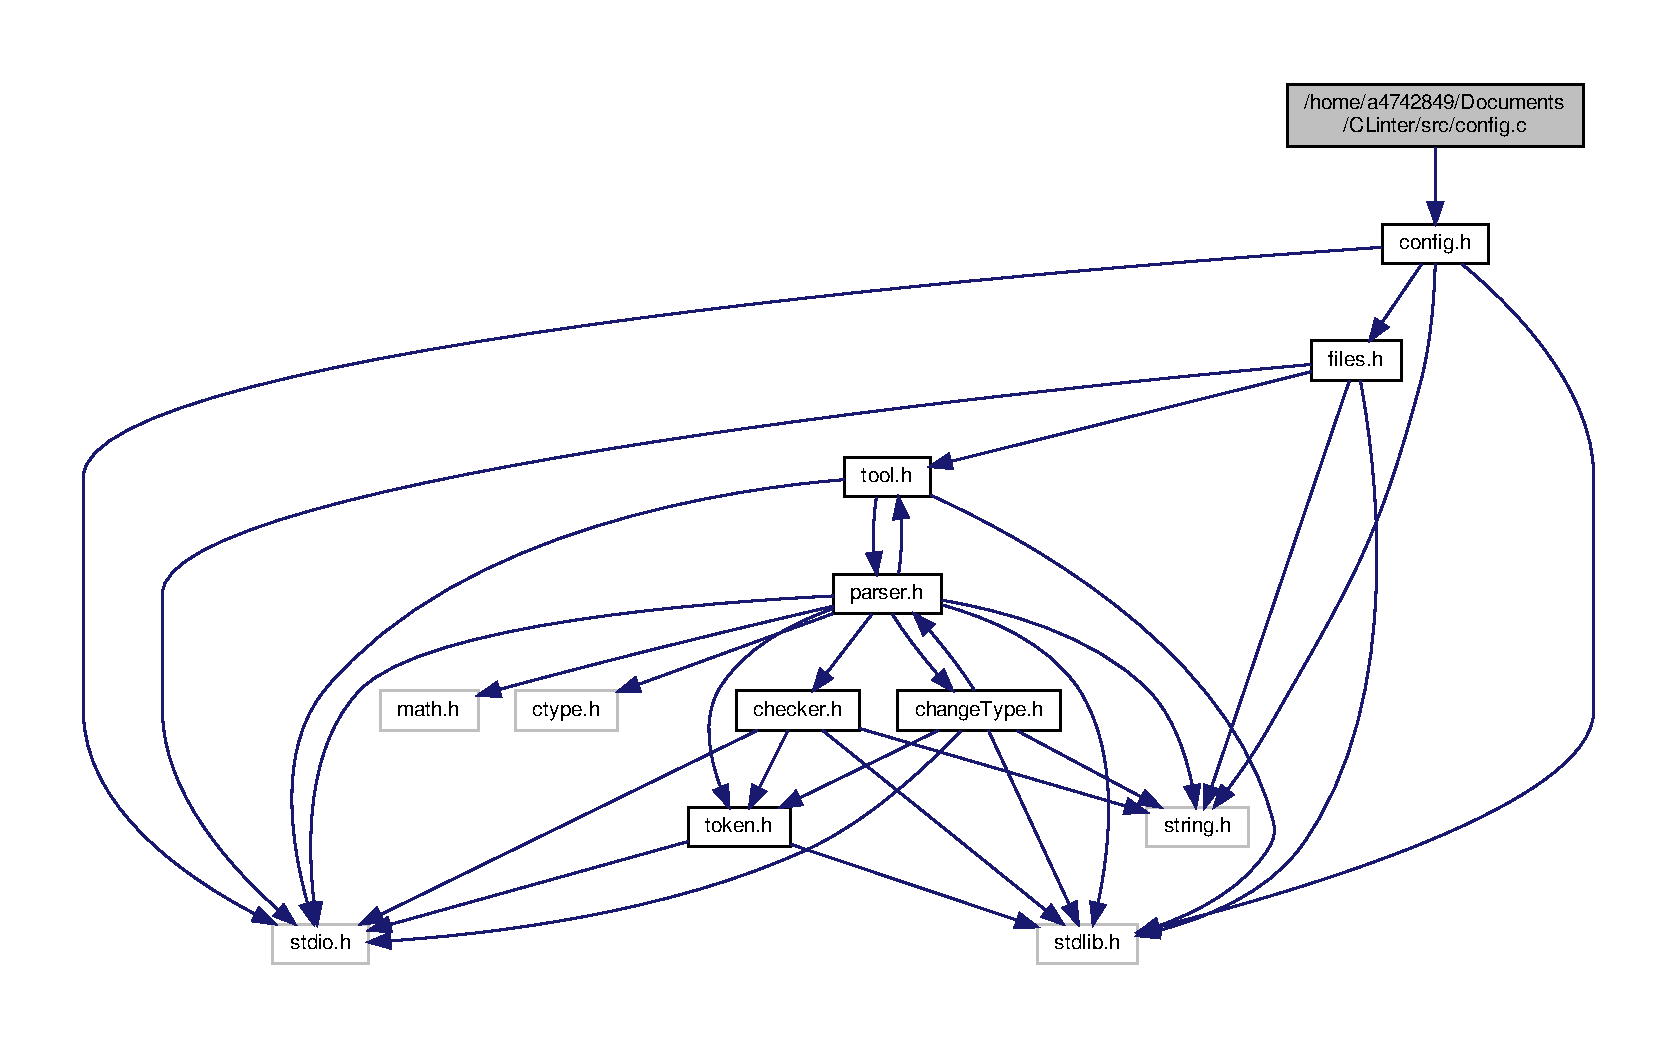
\includegraphics[width=350pt]{config_8c__incl}
\end{center}
\end{figure}
\subsection*{Functions}
\begin{DoxyCompactItemize}
\item 
char $\ast$$\ast$ \hyperlink{config_8c_a82020b88c3cb7b3a466111c664b75155}{merge\+Text} (char $\ast$$\ast$txt1, int $\ast$nb1, char $\ast$$\ast$txt2, int $\ast$nb2)
\begin{DoxyCompactList}\small\item\em Merge 2 texts content. \end{DoxyCompactList}\item 
char $\ast$ \hyperlink{config_8c_a28bfb244776a5451f78bcac5b8ec6243}{get\+Config\+File} (int argc, char $\ast$$\ast$argv)
\begin{DoxyCompactList}\small\item\em Get the Config File. \end{DoxyCompactList}\item 
int \hyperlink{config_8c_ad2e7ef347a4d034021d1566ea90cb0d0}{is\+Valid\+Conf\+File} (char $\ast$filename)
\begin{DoxyCompactList}\small\item\em Check if a given file has good name format. \end{DoxyCompactList}\item 
short \hyperlink{config_8c_a4d35009c11af9311968664a3a935b6f4}{get\+Recursive} (char $\ast$$\ast$file, int nb\+Lines)
\begin{DoxyCompactList}\small\item\em Get the Recursive option value. \end{DoxyCompactList}\item 
char $\ast$ \hyperlink{config_8c_a83d1ffc670b07f107d76c7cc14149dee}{get\+Extends} (char $\ast$$\ast$file, int nb\+Lines)
\begin{DoxyCompactList}\small\item\em Get the Extends file name. \end{DoxyCompactList}\item 
char $\ast$$\ast$ \hyperlink{config_8c_a9b64c40c31b3d2868db2b8c878cb1ccb}{get\+Files\+Name} (char $\ast$$\ast$file, int nb\+Lines, int $\ast$Nb\+Files)
\begin{DoxyCompactList}\small\item\em Get list of excluded files in lconf. \end{DoxyCompactList}\item 
int \hyperlink{config_8c_a59f7de2bafbfcb3bbda1c089065532ec}{get\+Val} (char $\ast$$\ast$file, char $\ast$rule, int nb\+Lines)
\begin{DoxyCompactList}\small\item\em Get the value of a field in a config. \end{DoxyCompactList}\item 
void \hyperlink{config_8c_ad850ee50eebe9ab9747ade7890133a19}{merge\+Conf} (\hyperlink{config_8h_a88ebb5d72d9993f342c6a9ae222a743c}{Config} $\ast$conf, char $\ast$path)
\begin{DoxyCompactList}\small\item\em Merge 2 configurations. \end{DoxyCompactList}\item 
\hyperlink{config_8h_a88ebb5d72d9993f342c6a9ae222a743c}{Config} $\ast$ \hyperlink{config_8c_a07a52dee4b7fa099a0e8a73c3a379ad1}{load\+Config} (char $\ast$path)
\begin{DoxyCompactList}\small\item\em Load the configuration from a file. \end{DoxyCompactList}\end{DoxyCompactItemize}


\subsection{Detailed Description}
This c file will contain all functions to load a lconf file. 

\begin{DoxyAuthor}{Author}
Antoine T\+A\+V\+E\+R\+N\+I\+ER
\end{DoxyAuthor}
\begin{DoxyDate}{Date}
16/11/2018 
\end{DoxyDate}


\subsection{Function Documentation}
\mbox{\Hypertarget{config_8c_a28bfb244776a5451f78bcac5b8ec6243}\label{config_8c_a28bfb244776a5451f78bcac5b8ec6243}} 
\index{config.\+c@{config.\+c}!get\+Config\+File@{get\+Config\+File}}
\index{get\+Config\+File@{get\+Config\+File}!config.\+c@{config.\+c}}
\subsubsection{\texorpdfstring{get\+Config\+File()}{getConfigFile()}}
{\footnotesize\ttfamily char $\ast$ get\+Config\+File (\begin{DoxyParamCaption}\item[{int}]{argc,  }\item[{char $\ast$$\ast$}]{argv }\end{DoxyParamCaption})}



Get the Config File. 


\begin{DoxyParams}{Parameters}
{\em argc} & Number of argument of main \\
\hline
{\em argv} & List of argument of main \\
\hline
\end{DoxyParams}
\begin{DoxyReturn}{Returns}
char$\ast$ Name of config file 
\end{DoxyReturn}
\mbox{\Hypertarget{config_8c_a83d1ffc670b07f107d76c7cc14149dee}\label{config_8c_a83d1ffc670b07f107d76c7cc14149dee}} 
\index{config.\+c@{config.\+c}!get\+Extends@{get\+Extends}}
\index{get\+Extends@{get\+Extends}!config.\+c@{config.\+c}}
\subsubsection{\texorpdfstring{get\+Extends()}{getExtends()}}
{\footnotesize\ttfamily char$\ast$ get\+Extends (\begin{DoxyParamCaption}\item[{char $\ast$$\ast$}]{file,  }\item[{int}]{nb\+Lines }\end{DoxyParamCaption})}



Get the Extends file name. 


\begin{DoxyParams}{Parameters}
{\em file} & List of Strings represented by a file \\
\hline
{\em nb\+Lines} & Number of lines in the file \\
\hline
\end{DoxyParams}
\begin{DoxyReturn}{Returns}
char$\ast$ A file name 
\end{DoxyReturn}
\mbox{\Hypertarget{config_8c_a9b64c40c31b3d2868db2b8c878cb1ccb}\label{config_8c_a9b64c40c31b3d2868db2b8c878cb1ccb}} 
\index{config.\+c@{config.\+c}!get\+Files\+Name@{get\+Files\+Name}}
\index{get\+Files\+Name@{get\+Files\+Name}!config.\+c@{config.\+c}}
\subsubsection{\texorpdfstring{get\+Files\+Name()}{getFilesName()}}
{\footnotesize\ttfamily char$\ast$$\ast$ get\+Files\+Name (\begin{DoxyParamCaption}\item[{char $\ast$$\ast$}]{file,  }\item[{int}]{nb\+Lines,  }\item[{int $\ast$}]{Nb\+Files }\end{DoxyParamCaption})}



Get list of excluded files in lconf. 


\begin{DoxyParams}{Parameters}
{\em file} & List of Strings represented by a file \\
\hline
{\em nb\+Lines} & Number of lines in the file \\
\hline
{\em Nb\+Files} & Number of excluded files updated \\
\hline
\end{DoxyParams}
\begin{DoxyReturn}{Returns}
char$\ast$$\ast$ List of files name 
\end{DoxyReturn}
\mbox{\Hypertarget{config_8c_a4d35009c11af9311968664a3a935b6f4}\label{config_8c_a4d35009c11af9311968664a3a935b6f4}} 
\index{config.\+c@{config.\+c}!get\+Recursive@{get\+Recursive}}
\index{get\+Recursive@{get\+Recursive}!config.\+c@{config.\+c}}
\subsubsection{\texorpdfstring{get\+Recursive()}{getRecursive()}}
{\footnotesize\ttfamily short get\+Recursive (\begin{DoxyParamCaption}\item[{char $\ast$$\ast$}]{file,  }\item[{int}]{nb\+Lines }\end{DoxyParamCaption})}



Get the Recursive option value. 


\begin{DoxyParams}{Parameters}
{\em file} & List of Strings represented by a file \\
\hline
{\em nb\+Lines} & Number of lines in the file \\
\hline
\end{DoxyParams}
\begin{DoxyReturn}{Returns}
short 0 false else true 
\end{DoxyReturn}
\mbox{\Hypertarget{config_8c_a59f7de2bafbfcb3bbda1c089065532ec}\label{config_8c_a59f7de2bafbfcb3bbda1c089065532ec}} 
\index{config.\+c@{config.\+c}!get\+Val@{get\+Val}}
\index{get\+Val@{get\+Val}!config.\+c@{config.\+c}}
\subsubsection{\texorpdfstring{get\+Val()}{getVal()}}
{\footnotesize\ttfamily int get\+Val (\begin{DoxyParamCaption}\item[{char $\ast$$\ast$}]{file,  }\item[{char $\ast$}]{rule,  }\item[{int}]{nb\+Lines }\end{DoxyParamCaption})}



Get the value of a field in a config. 


\begin{DoxyParams}{Parameters}
{\em file} & List of Strings represented by a file \\
\hline
{\em rule} & String representation of a rule in the lconf file \\
\hline
{\em nb\+Lines} & Number of lines in the lconf file \\
\hline
\end{DoxyParams}
\begin{DoxyReturn}{Returns}
int 0 false else true 
\end{DoxyReturn}
\mbox{\Hypertarget{config_8c_ad2e7ef347a4d034021d1566ea90cb0d0}\label{config_8c_ad2e7ef347a4d034021d1566ea90cb0d0}} 
\index{config.\+c@{config.\+c}!is\+Valid\+Conf\+File@{is\+Valid\+Conf\+File}}
\index{is\+Valid\+Conf\+File@{is\+Valid\+Conf\+File}!config.\+c@{config.\+c}}
\subsubsection{\texorpdfstring{is\+Valid\+Conf\+File()}{isValidConfFile()}}
{\footnotesize\ttfamily int is\+Valid\+Conf\+File (\begin{DoxyParamCaption}\item[{char $\ast$}]{filename }\end{DoxyParamCaption})}



Check if a given file has good name format. 


\begin{DoxyParams}{Parameters}
{\em filename} & A file path \\
\hline
\end{DoxyParams}
\begin{DoxyReturn}{Returns}
int false (0) if not contains .lconf else true (1) 
\end{DoxyReturn}
\mbox{\Hypertarget{config_8c_a07a52dee4b7fa099a0e8a73c3a379ad1}\label{config_8c_a07a52dee4b7fa099a0e8a73c3a379ad1}} 
\index{config.\+c@{config.\+c}!load\+Config@{load\+Config}}
\index{load\+Config@{load\+Config}!config.\+c@{config.\+c}}
\subsubsection{\texorpdfstring{load\+Config()}{loadConfig()}}
{\footnotesize\ttfamily \hyperlink{config_8h_a88ebb5d72d9993f342c6a9ae222a743c}{Config}$\ast$ load\+Config (\begin{DoxyParamCaption}\item[{char $\ast$}]{path }\end{DoxyParamCaption})}



Load the configuration from a file. 


\begin{DoxyParams}{Parameters}
{\em path} & Configuration file \\
\hline
\end{DoxyParams}
\begin{DoxyReturn}{Returns}
Config$\ast$ Configuration structure from given file 
\end{DoxyReturn}
\mbox{\Hypertarget{config_8c_ad850ee50eebe9ab9747ade7890133a19}\label{config_8c_ad850ee50eebe9ab9747ade7890133a19}} 
\index{config.\+c@{config.\+c}!merge\+Conf@{merge\+Conf}}
\index{merge\+Conf@{merge\+Conf}!config.\+c@{config.\+c}}
\subsubsection{\texorpdfstring{merge\+Conf()}{mergeConf()}}
{\footnotesize\ttfamily void merge\+Conf (\begin{DoxyParamCaption}\item[{\hyperlink{config_8h_a88ebb5d72d9993f342c6a9ae222a743c}{Config} $\ast$}]{conf,  }\item[{char $\ast$}]{path }\end{DoxyParamCaption})}



Merge 2 configurations. 


\begin{DoxyParams}{Parameters}
{\em conf} & Original configuration structure \\
\hline
{\em path} & The path to the new configuration to merge with the original structure \\
\hline
\end{DoxyParams}
\mbox{\Hypertarget{config_8c_a82020b88c3cb7b3a466111c664b75155}\label{config_8c_a82020b88c3cb7b3a466111c664b75155}} 
\index{config.\+c@{config.\+c}!merge\+Text@{merge\+Text}}
\index{merge\+Text@{merge\+Text}!config.\+c@{config.\+c}}
\subsubsection{\texorpdfstring{merge\+Text()}{mergeText()}}
{\footnotesize\ttfamily char$\ast$$\ast$ merge\+Text (\begin{DoxyParamCaption}\item[{char $\ast$$\ast$}]{txt1,  }\item[{int $\ast$}]{nb1,  }\item[{char $\ast$$\ast$}]{txt2,  }\item[{int $\ast$}]{nb2 }\end{DoxyParamCaption})}



Merge 2 texts content. 


\begin{DoxyParams}{Parameters}
{\em txt1} & List of strings 1 \\
\hline
{\em nb1} & Number of strings in 1, updated with sum of nb1, nb2 \\
\hline
{\em txt2} & List of strings 2 \\
\hline
{\em nb2} & Number of strings in 2 \\
\hline
\end{DoxyParams}
\begin{DoxyReturn}{Returns}
char$\ast$$\ast$ The total content of both texts 
\end{DoxyReturn}

\hypertarget{config_8h}{}\section{/home/a4742849/\+Documents/\+C\+Linter/src/config.h File Reference}
\label{config_8h}\index{/home/a4742849/\+Documents/\+C\+Linter/src/config.\+h@{/home/a4742849/\+Documents/\+C\+Linter/src/config.\+h}}


This header file will contain all required definitions and basic utilities functions to read and load a configuration file.  


{\ttfamily \#include $<$stdlib.\+h$>$}\newline
{\ttfamily \#include $<$stdio.\+h$>$}\newline
{\ttfamily \#include $<$string.\+h$>$}\newline
{\ttfamily \#include \char`\"{}files.\+h\char`\"{}}\newline
Include dependency graph for config.\+h\+:\nopagebreak
\begin{figure}[H]
\begin{center}
\leavevmode
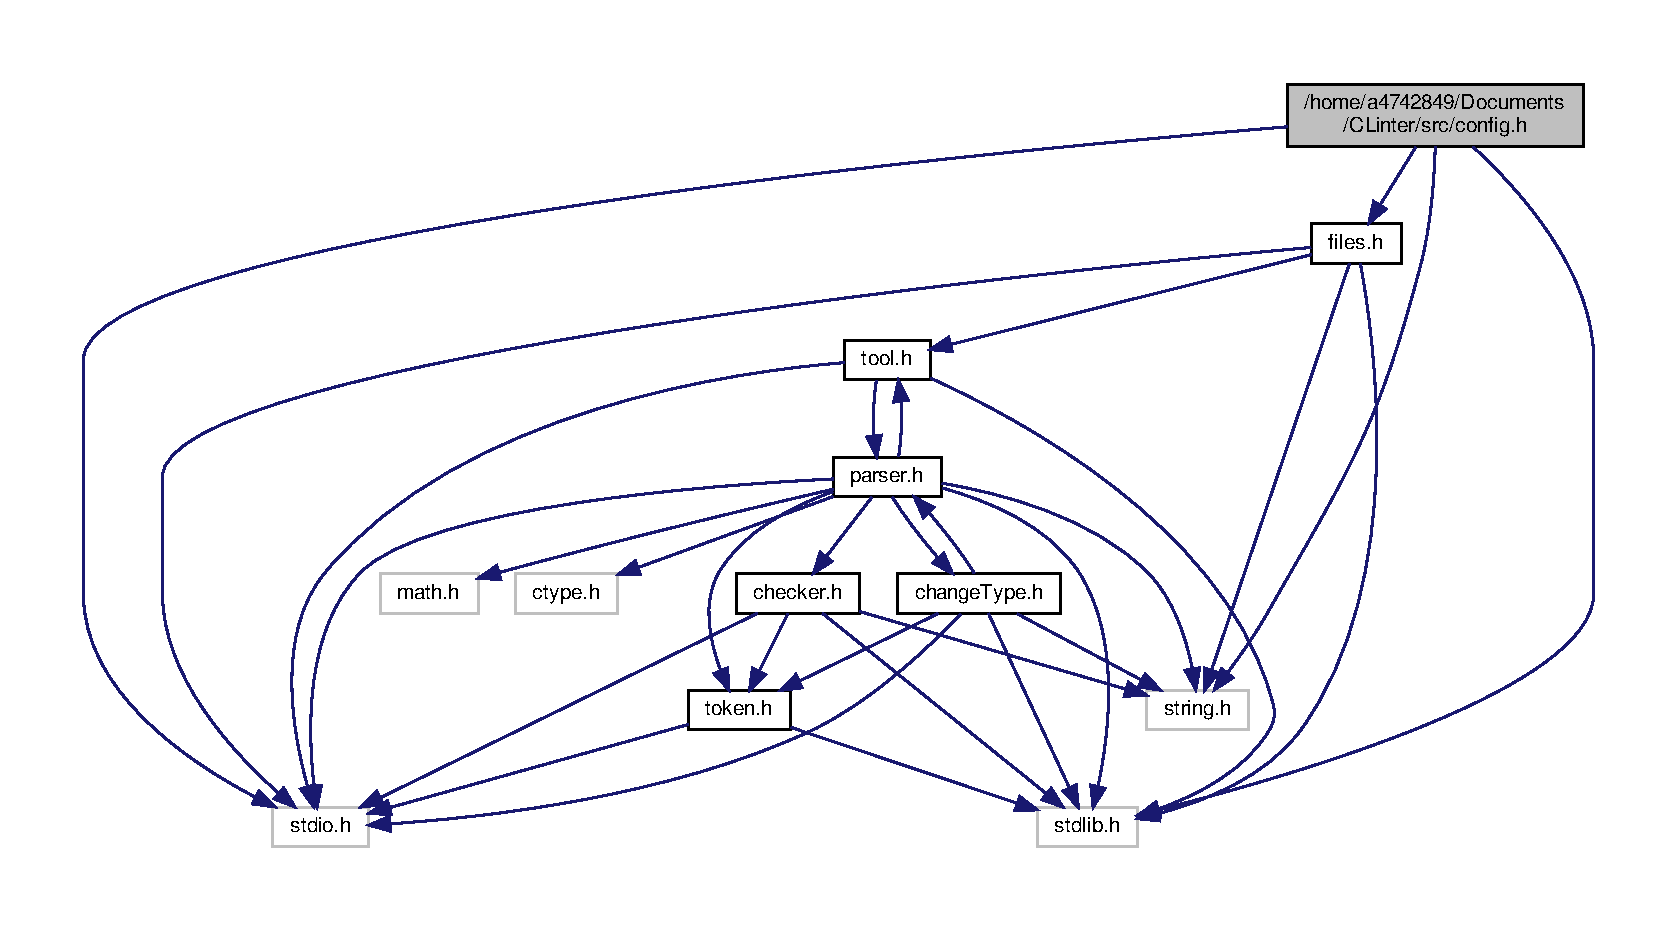
\includegraphics[width=350pt]{config_8h__incl}
\end{center}
\end{figure}
This graph shows which files directly or indirectly include this file\+:
\nopagebreak
\begin{figure}[H]
\begin{center}
\leavevmode
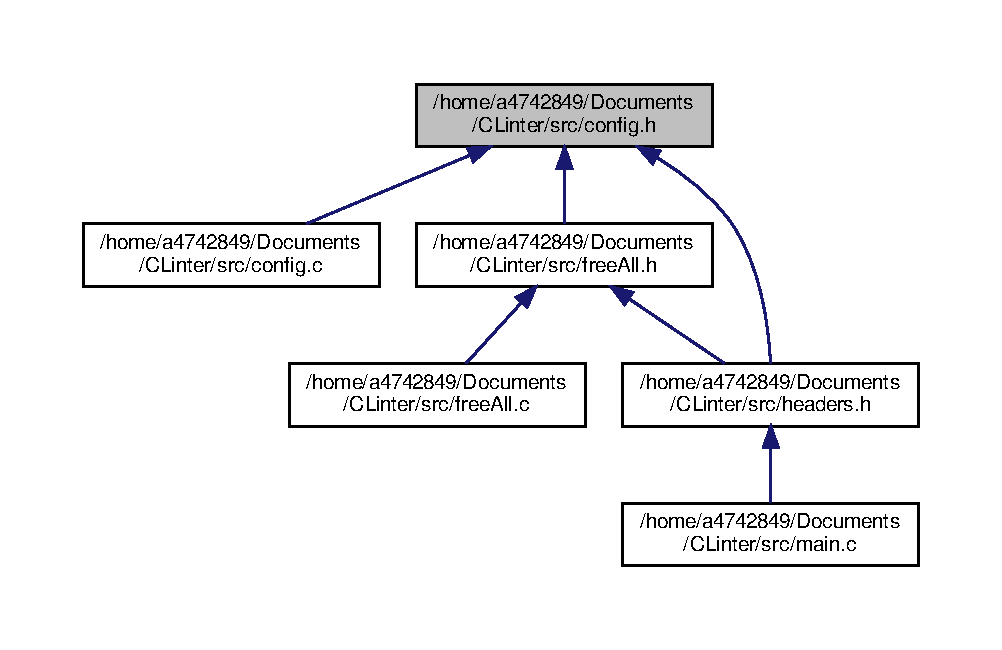
\includegraphics[width=350pt]{config_8h__dep__incl}
\end{center}
\end{figure}
\subsection*{Classes}
\begin{DoxyCompactItemize}
\item 
struct \hyperlink{structConfig__t}{Config\+\_\+t}
\begin{DoxyCompactList}\small\item\em Structure to store all configurations elements. \end{DoxyCompactList}\end{DoxyCompactItemize}
\subsection*{Macros}
\begin{DoxyCompactItemize}
\item 
\#define \hyperlink{config_8h_aacc3ee1a7f283f8ef65cea31f4436a95}{M\+AX}(x,  y)~(((x) $>$ (y)) ? (x) \+: (y))
\begin{DoxyCompactList}\small\item\em Macro to return M\+AX between integers. \end{DoxyCompactList}\end{DoxyCompactItemize}
\subsection*{Typedefs}
\begin{DoxyCompactItemize}
\item 
typedef struct \hyperlink{structConfig__t}{Config\+\_\+t} \hyperlink{config_8h_a88ebb5d72d9993f342c6a9ae222a743c}{Config}
\begin{DoxyCompactList}\small\item\em Structure to store all configurations elements. \end{DoxyCompactList}\end{DoxyCompactItemize}
\subsection*{Functions}
\begin{DoxyCompactItemize}
\item 
char $\ast$$\ast$ \hyperlink{config_8h_a82020b88c3cb7b3a466111c664b75155}{merge\+Text} (char $\ast$$\ast$txt1, int $\ast$nb1, char $\ast$$\ast$txt2, int $\ast$nb2)
\begin{DoxyCompactList}\small\item\em Merge 2 texts content. \end{DoxyCompactList}\item 
char $\ast$ \hyperlink{config_8h_a868aab2fe8394b0008a7f1118fbc1785}{get\+Config\+File} (int argc, char $\ast$$\ast$argv)
\begin{DoxyCompactList}\small\item\em Get the Config File. \end{DoxyCompactList}\item 
int \hyperlink{config_8h_ad2e7ef347a4d034021d1566ea90cb0d0}{is\+Valid\+Conf\+File} (char $\ast$filename)
\begin{DoxyCompactList}\small\item\em Check if a given file has good name format. \end{DoxyCompactList}\item 
short \hyperlink{config_8h_a4d35009c11af9311968664a3a935b6f4}{get\+Recursive} (char $\ast$$\ast$file, int nb\+Lines)
\begin{DoxyCompactList}\small\item\em Get the Recursive option value. \end{DoxyCompactList}\item 
char $\ast$ \hyperlink{config_8h_a83d1ffc670b07f107d76c7cc14149dee}{get\+Extends} (char $\ast$$\ast$file, int nb\+Lines)
\begin{DoxyCompactList}\small\item\em Get the Extends file name. \end{DoxyCompactList}\item 
char $\ast$$\ast$ \hyperlink{config_8h_a9b64c40c31b3d2868db2b8c878cb1ccb}{get\+Files\+Name} (char $\ast$$\ast$file, int nb\+Lines, int $\ast$Nb\+Files)
\begin{DoxyCompactList}\small\item\em Get list of excluded files in lconf. \end{DoxyCompactList}\item 
int \hyperlink{config_8h_a59f7de2bafbfcb3bbda1c089065532ec}{get\+Val} (char $\ast$$\ast$file, char $\ast$rule, int nb\+Lines)
\begin{DoxyCompactList}\small\item\em Get the value of a field in a config. \end{DoxyCompactList}\item 
\hyperlink{config_8h_a88ebb5d72d9993f342c6a9ae222a743c}{Config} $\ast$ \hyperlink{config_8h_a07a52dee4b7fa099a0e8a73c3a379ad1}{load\+Config} (char $\ast$path)
\begin{DoxyCompactList}\small\item\em Load the configuration from a file. \end{DoxyCompactList}\end{DoxyCompactItemize}


\subsection{Detailed Description}
This header file will contain all required definitions and basic utilities functions to read and load a configuration file. 

\begin{DoxyAuthor}{Author}
Antoine T\+A\+V\+E\+R\+N\+I\+ER
\end{DoxyAuthor}
\begin{DoxyDate}{Date}
16/11/2018 
\end{DoxyDate}


\subsection{Macro Definition Documentation}
\mbox{\Hypertarget{config_8h_aacc3ee1a7f283f8ef65cea31f4436a95}\label{config_8h_aacc3ee1a7f283f8ef65cea31f4436a95}} 
\index{config.\+h@{config.\+h}!M\+AX@{M\+AX}}
\index{M\+AX@{M\+AX}!config.\+h@{config.\+h}}
\subsubsection{\texorpdfstring{M\+AX}{MAX}}
{\footnotesize\ttfamily \#define M\+AX(\begin{DoxyParamCaption}\item[{}]{x,  }\item[{}]{y }\end{DoxyParamCaption})~(((x) $>$ (y)) ? (x) \+: (y))}



Macro to return M\+AX between integers. 



\subsection{Typedef Documentation}
\mbox{\Hypertarget{config_8h_a88ebb5d72d9993f342c6a9ae222a743c}\label{config_8h_a88ebb5d72d9993f342c6a9ae222a743c}} 
\index{config.\+h@{config.\+h}!Config@{Config}}
\index{Config@{Config}!config.\+h@{config.\+h}}
\subsubsection{\texorpdfstring{Config}{Config}}
{\footnotesize\ttfamily typedef struct \hyperlink{structConfig__t}{Config\+\_\+t}  \hyperlink{config_8h_a88ebb5d72d9993f342c6a9ae222a743c}{Config}}



Structure to store all configurations elements. 



\subsection{Function Documentation}
\mbox{\Hypertarget{config_8h_a868aab2fe8394b0008a7f1118fbc1785}\label{config_8h_a868aab2fe8394b0008a7f1118fbc1785}} 
\index{config.\+h@{config.\+h}!get\+Config\+File@{get\+Config\+File}}
\index{get\+Config\+File@{get\+Config\+File}!config.\+h@{config.\+h}}
\subsubsection{\texorpdfstring{get\+Config\+File()}{getConfigFile()}}
{\footnotesize\ttfamily char$\ast$ get\+Config\+File (\begin{DoxyParamCaption}\item[{int}]{argc,  }\item[{char $\ast$$\ast$}]{argv }\end{DoxyParamCaption})}



Get the Config File. 


\begin{DoxyParams}{Parameters}
{\em argc} & Number of argument of main \\
\hline
{\em argv} & List of argument of main \\
\hline
\end{DoxyParams}
\begin{DoxyReturn}{Returns}
char$\ast$ Name of config file 
\end{DoxyReturn}
\mbox{\Hypertarget{config_8h_a83d1ffc670b07f107d76c7cc14149dee}\label{config_8h_a83d1ffc670b07f107d76c7cc14149dee}} 
\index{config.\+h@{config.\+h}!get\+Extends@{get\+Extends}}
\index{get\+Extends@{get\+Extends}!config.\+h@{config.\+h}}
\subsubsection{\texorpdfstring{get\+Extends()}{getExtends()}}
{\footnotesize\ttfamily char$\ast$ get\+Extends (\begin{DoxyParamCaption}\item[{char $\ast$$\ast$}]{file,  }\item[{int}]{nb\+Lines }\end{DoxyParamCaption})}



Get the Extends file name. 


\begin{DoxyParams}{Parameters}
{\em file} & List of Strings represented by a file \\
\hline
{\em nb\+Lines} & Number of lines in the file \\
\hline
\end{DoxyParams}
\begin{DoxyReturn}{Returns}
char$\ast$ A file name 
\end{DoxyReturn}
\mbox{\Hypertarget{config_8h_a9b64c40c31b3d2868db2b8c878cb1ccb}\label{config_8h_a9b64c40c31b3d2868db2b8c878cb1ccb}} 
\index{config.\+h@{config.\+h}!get\+Files\+Name@{get\+Files\+Name}}
\index{get\+Files\+Name@{get\+Files\+Name}!config.\+h@{config.\+h}}
\subsubsection{\texorpdfstring{get\+Files\+Name()}{getFilesName()}}
{\footnotesize\ttfamily char$\ast$$\ast$ get\+Files\+Name (\begin{DoxyParamCaption}\item[{char $\ast$$\ast$}]{file,  }\item[{int}]{nb\+Lines,  }\item[{int $\ast$}]{Nb\+Files }\end{DoxyParamCaption})}



Get list of excluded files in lconf. 


\begin{DoxyParams}{Parameters}
{\em file} & List of Strings represented by a file \\
\hline
{\em nb\+Lines} & Number of lines in the file \\
\hline
{\em Nb\+Files} & Number of excluded files updated \\
\hline
\end{DoxyParams}
\begin{DoxyReturn}{Returns}
char$\ast$$\ast$ List of files name 
\end{DoxyReturn}
\mbox{\Hypertarget{config_8h_a4d35009c11af9311968664a3a935b6f4}\label{config_8h_a4d35009c11af9311968664a3a935b6f4}} 
\index{config.\+h@{config.\+h}!get\+Recursive@{get\+Recursive}}
\index{get\+Recursive@{get\+Recursive}!config.\+h@{config.\+h}}
\subsubsection{\texorpdfstring{get\+Recursive()}{getRecursive()}}
{\footnotesize\ttfamily short get\+Recursive (\begin{DoxyParamCaption}\item[{char $\ast$$\ast$}]{file,  }\item[{int}]{nb\+Lines }\end{DoxyParamCaption})}



Get the Recursive option value. 


\begin{DoxyParams}{Parameters}
{\em file} & List of Strings represented by a file \\
\hline
{\em nb\+Lines} & Number of lines in the file \\
\hline
\end{DoxyParams}
\begin{DoxyReturn}{Returns}
short 0 false else true 
\end{DoxyReturn}
\mbox{\Hypertarget{config_8h_a59f7de2bafbfcb3bbda1c089065532ec}\label{config_8h_a59f7de2bafbfcb3bbda1c089065532ec}} 
\index{config.\+h@{config.\+h}!get\+Val@{get\+Val}}
\index{get\+Val@{get\+Val}!config.\+h@{config.\+h}}
\subsubsection{\texorpdfstring{get\+Val()}{getVal()}}
{\footnotesize\ttfamily int get\+Val (\begin{DoxyParamCaption}\item[{char $\ast$$\ast$}]{file,  }\item[{char $\ast$}]{rule,  }\item[{int}]{nb\+Lines }\end{DoxyParamCaption})}



Get the value of a field in a config. 


\begin{DoxyParams}{Parameters}
{\em file} & List of Strings represented by a file \\
\hline
{\em rule} & String representation of a rule in the lconf file \\
\hline
{\em nb\+Lines} & Number of lines in the lconf file \\
\hline
\end{DoxyParams}
\begin{DoxyReturn}{Returns}
int 0 false else true 
\end{DoxyReturn}
\mbox{\Hypertarget{config_8h_ad2e7ef347a4d034021d1566ea90cb0d0}\label{config_8h_ad2e7ef347a4d034021d1566ea90cb0d0}} 
\index{config.\+h@{config.\+h}!is\+Valid\+Conf\+File@{is\+Valid\+Conf\+File}}
\index{is\+Valid\+Conf\+File@{is\+Valid\+Conf\+File}!config.\+h@{config.\+h}}
\subsubsection{\texorpdfstring{is\+Valid\+Conf\+File()}{isValidConfFile()}}
{\footnotesize\ttfamily int is\+Valid\+Conf\+File (\begin{DoxyParamCaption}\item[{char $\ast$}]{filename }\end{DoxyParamCaption})}



Check if a given file has good name format. 


\begin{DoxyParams}{Parameters}
{\em filename} & A file path \\
\hline
\end{DoxyParams}
\begin{DoxyReturn}{Returns}
int false (0) if not contains .lconf else true (1) 
\end{DoxyReturn}
\mbox{\Hypertarget{config_8h_a07a52dee4b7fa099a0e8a73c3a379ad1}\label{config_8h_a07a52dee4b7fa099a0e8a73c3a379ad1}} 
\index{config.\+h@{config.\+h}!load\+Config@{load\+Config}}
\index{load\+Config@{load\+Config}!config.\+h@{config.\+h}}
\subsubsection{\texorpdfstring{load\+Config()}{loadConfig()}}
{\footnotesize\ttfamily \hyperlink{config_8h_a88ebb5d72d9993f342c6a9ae222a743c}{Config}$\ast$ load\+Config (\begin{DoxyParamCaption}\item[{char $\ast$}]{path }\end{DoxyParamCaption})}



Load the configuration from a file. 


\begin{DoxyParams}{Parameters}
{\em path} & Configuration file \\
\hline
\end{DoxyParams}
\begin{DoxyReturn}{Returns}
Config$\ast$ Configuration structure from given file 
\end{DoxyReturn}
\mbox{\Hypertarget{config_8h_a82020b88c3cb7b3a466111c664b75155}\label{config_8h_a82020b88c3cb7b3a466111c664b75155}} 
\index{config.\+h@{config.\+h}!merge\+Text@{merge\+Text}}
\index{merge\+Text@{merge\+Text}!config.\+h@{config.\+h}}
\subsubsection{\texorpdfstring{merge\+Text()}{mergeText()}}
{\footnotesize\ttfamily char$\ast$$\ast$ merge\+Text (\begin{DoxyParamCaption}\item[{char $\ast$$\ast$}]{txt1,  }\item[{int $\ast$}]{nb1,  }\item[{char $\ast$$\ast$}]{txt2,  }\item[{int $\ast$}]{nb2 }\end{DoxyParamCaption})}



Merge 2 texts content. 


\begin{DoxyParams}{Parameters}
{\em txt1} & List of strings 1 \\
\hline
{\em nb1} & Number of strings in 1, updated with sum of nb1, nb2 \\
\hline
{\em txt2} & List of strings 2 \\
\hline
{\em nb2} & Number of strings in 2 \\
\hline
\end{DoxyParams}
\begin{DoxyReturn}{Returns}
char$\ast$$\ast$ The total content of both texts 
\end{DoxyReturn}

\hypertarget{files_8c}{}\section{/home/a4742849/\+Documents/\+C\+Linter/src/files.c File Reference}
\label{files_8c}\index{/home/a4742849/\+Documents/\+C\+Linter/src/files.\+c@{/home/a4742849/\+Documents/\+C\+Linter/src/files.\+c}}


This c file will contain all functions to load a file in a char$\ast$$\ast$.  


{\ttfamily \#include \char`\"{}files.\+h\char`\"{}}\newline
Include dependency graph for files.\+c\+:\nopagebreak
\begin{figure}[H]
\begin{center}
\leavevmode
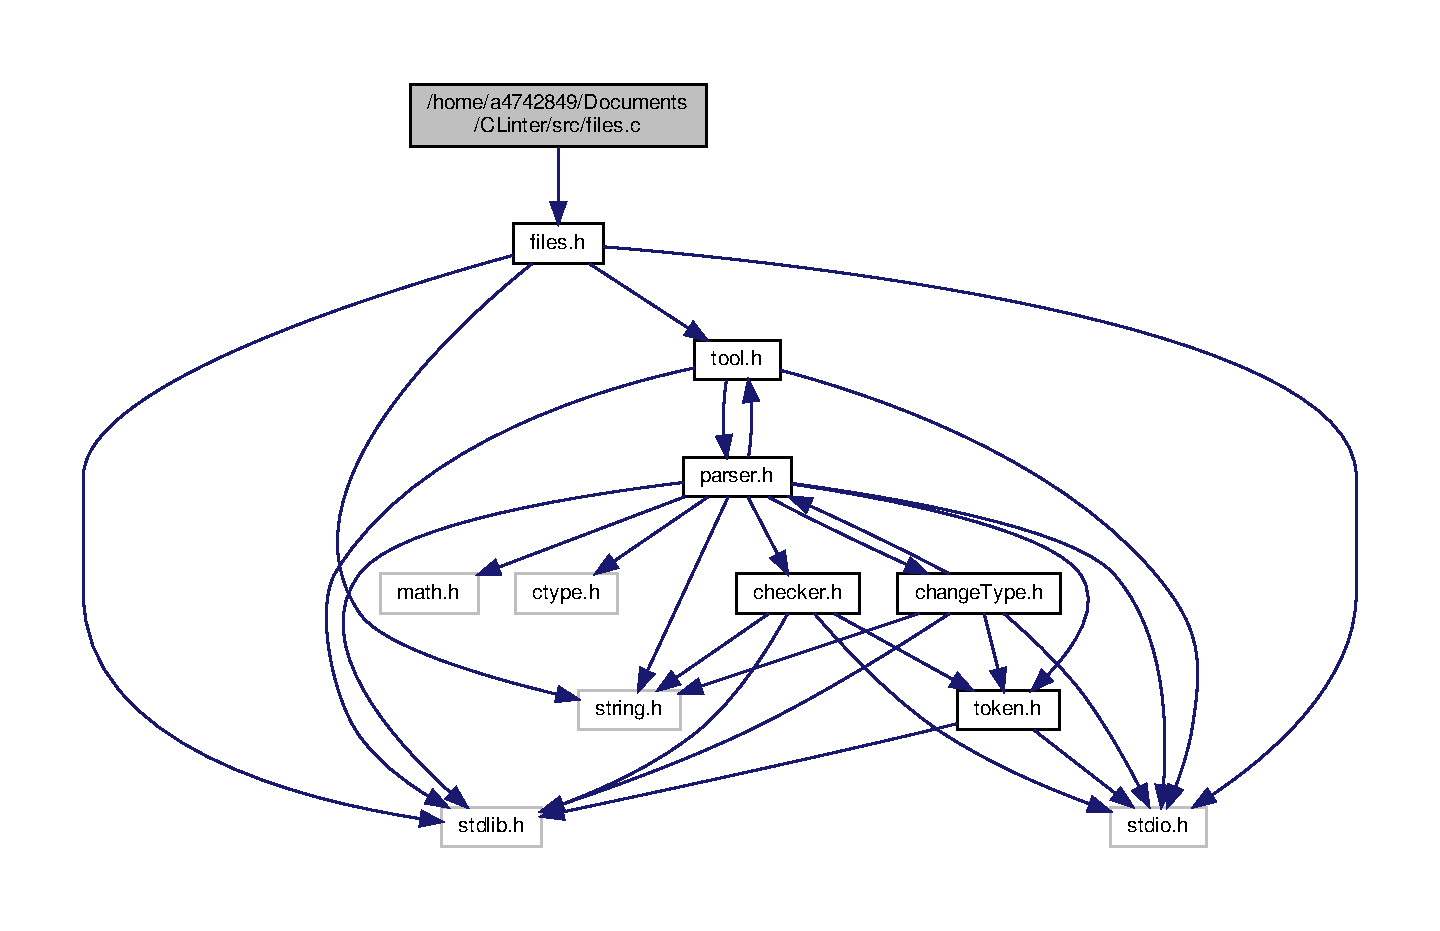
\includegraphics[width=350pt]{files_8c__incl}
\end{center}
\end{figure}
\subsection*{Functions}
\begin{DoxyCompactItemize}
\item 
int \hyperlink{files_8c_a35e14b890e4734b5d9d303bef756b965}{count\+Lines\+In\+File} (F\+I\+LE $\ast$f)
\begin{DoxyCompactList}\small\item\em Get the number of lines in a file. \end{DoxyCompactList}\item 
char $\ast$$\ast$ \hyperlink{files_8c_a91f0ab03ed084ddfee5ee7a8323d5dc1}{get\+All\+Lines} (char $\ast$path, int $\ast$nb\+Lines)
\begin{DoxyCompactList}\small\item\em Get the All Lines in a file. \end{DoxyCompactList}\end{DoxyCompactItemize}


\subsection{Detailed Description}
This c file will contain all functions to load a file in a char$\ast$$\ast$. 

\begin{DoxyAuthor}{Author}
Antoine T\+A\+V\+E\+R\+N\+I\+ER
\end{DoxyAuthor}
\begin{DoxyDate}{Date}
16/11/2018 
\end{DoxyDate}


\subsection{Function Documentation}
\mbox{\Hypertarget{files_8c_a35e14b890e4734b5d9d303bef756b965}\label{files_8c_a35e14b890e4734b5d9d303bef756b965}} 
\index{files.\+c@{files.\+c}!count\+Lines\+In\+File@{count\+Lines\+In\+File}}
\index{count\+Lines\+In\+File@{count\+Lines\+In\+File}!files.\+c@{files.\+c}}
\subsubsection{\texorpdfstring{count\+Lines\+In\+File()}{countLinesInFile()}}
{\footnotesize\ttfamily int count\+Lines\+In\+File (\begin{DoxyParamCaption}\item[{F\+I\+LE $\ast$}]{f }\end{DoxyParamCaption})}



Get the number of lines in a file. 


\begin{DoxyParams}{Parameters}
{\em f} & Given F\+I\+LE \\
\hline
\end{DoxyParams}
\begin{DoxyReturn}{Returns}
int Number of line in F\+I\+LE f 
\end{DoxyReturn}
\mbox{\Hypertarget{files_8c_a91f0ab03ed084ddfee5ee7a8323d5dc1}\label{files_8c_a91f0ab03ed084ddfee5ee7a8323d5dc1}} 
\index{files.\+c@{files.\+c}!get\+All\+Lines@{get\+All\+Lines}}
\index{get\+All\+Lines@{get\+All\+Lines}!files.\+c@{files.\+c}}
\subsubsection{\texorpdfstring{get\+All\+Lines()}{getAllLines()}}
{\footnotesize\ttfamily char$\ast$$\ast$ get\+All\+Lines (\begin{DoxyParamCaption}\item[{char $\ast$}]{path,  }\item[{int $\ast$}]{nb\+Lines }\end{DoxyParamCaption})}



Get the All Lines in a file. 


\begin{DoxyParams}{Parameters}
{\em path} & Path of file \\
\hline
{\em nb\+Lines} & Number of lines updated in the file \\
\hline
\end{DoxyParams}
\begin{DoxyReturn}{Returns}
char$\ast$$\ast$ A list of string containing the text of file 
\end{DoxyReturn}

\hypertarget{files_8h}{}\section{/home/a4742849/\+Documents/\+C\+Linter/src/files.h File Reference}
\label{files_8h}\index{/home/a4742849/\+Documents/\+C\+Linter/src/files.\+h@{/home/a4742849/\+Documents/\+C\+Linter/src/files.\+h}}


This header file will contain all required definitions and basic utilities functions to read and load a file into a char$\ast$$\ast$.  


{\ttfamily \#include $<$stdlib.\+h$>$}\newline
{\ttfamily \#include $<$stdio.\+h$>$}\newline
{\ttfamily \#include $<$string.\+h$>$}\newline
{\ttfamily \#include \char`\"{}tool.\+h\char`\"{}}\newline
Include dependency graph for files.\+h\+:\nopagebreak
\begin{figure}[H]
\begin{center}
\leavevmode
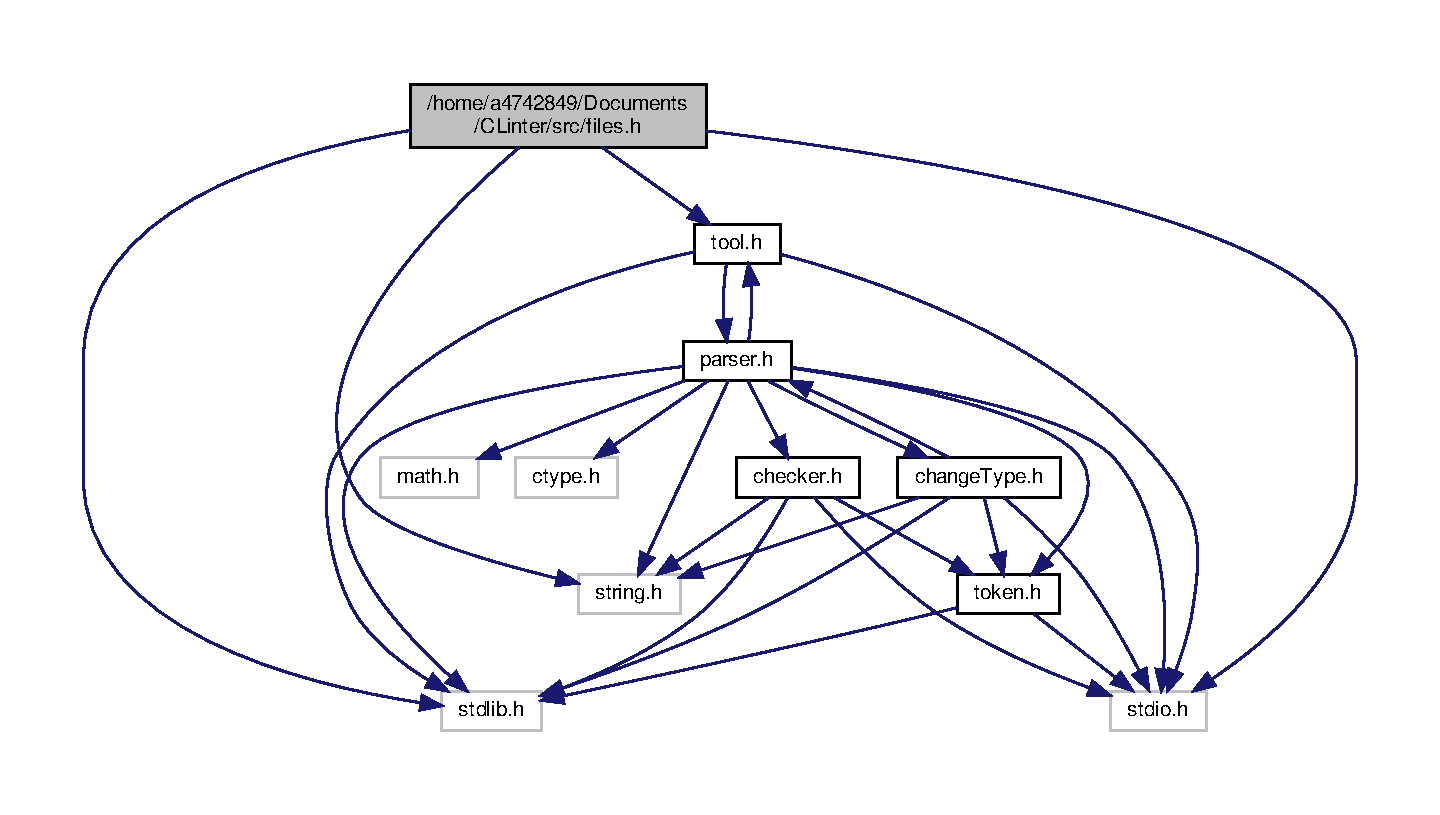
\includegraphics[width=350pt]{files_8h__incl}
\end{center}
\end{figure}
This graph shows which files directly or indirectly include this file\+:
\nopagebreak
\begin{figure}[H]
\begin{center}
\leavevmode
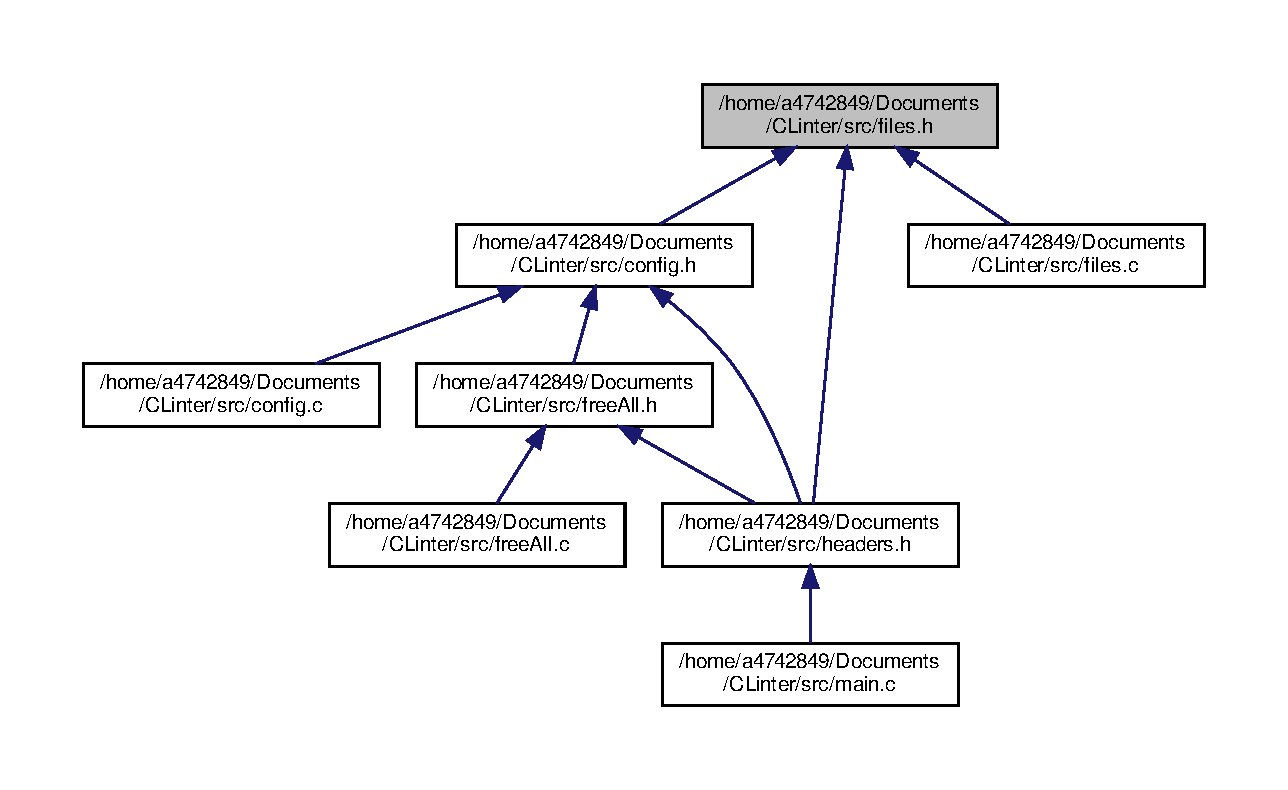
\includegraphics[width=350pt]{files_8h__dep__incl}
\end{center}
\end{figure}
\subsection*{Macros}
\begin{DoxyCompactItemize}
\item 
\#define \hyperlink{files_8h_a369266c24eacffb87046522897a570d5}{\+\_\+\+G\+N\+U\+\_\+\+S\+O\+U\+R\+CE}
\end{DoxyCompactItemize}
\subsection*{Functions}
\begin{DoxyCompactItemize}
\item 
int \hyperlink{files_8h_a35e14b890e4734b5d9d303bef756b965}{count\+Lines\+In\+File} (F\+I\+LE $\ast$f)
\begin{DoxyCompactList}\small\item\em Get the number of lines in a file. \end{DoxyCompactList}\item 
char $\ast$$\ast$ \hyperlink{files_8h_a91f0ab03ed084ddfee5ee7a8323d5dc1}{get\+All\+Lines} (char $\ast$path, int $\ast$nb\+Lines)
\begin{DoxyCompactList}\small\item\em Get the All Lines in a file. \end{DoxyCompactList}\end{DoxyCompactItemize}


\subsection{Detailed Description}
This header file will contain all required definitions and basic utilities functions to read and load a file into a char$\ast$$\ast$. 

\begin{DoxyAuthor}{Author}
Antoine T\+A\+V\+E\+R\+N\+I\+ER
\end{DoxyAuthor}
\begin{DoxyDate}{Date}
16/11/2018 
\end{DoxyDate}


\subsection{Macro Definition Documentation}
\mbox{\Hypertarget{files_8h_a369266c24eacffb87046522897a570d5}\label{files_8h_a369266c24eacffb87046522897a570d5}} 
\index{files.\+h@{files.\+h}!\+\_\+\+G\+N\+U\+\_\+\+S\+O\+U\+R\+CE@{\+\_\+\+G\+N\+U\+\_\+\+S\+O\+U\+R\+CE}}
\index{\+\_\+\+G\+N\+U\+\_\+\+S\+O\+U\+R\+CE@{\+\_\+\+G\+N\+U\+\_\+\+S\+O\+U\+R\+CE}!files.\+h@{files.\+h}}
\subsubsection{\texorpdfstring{\+\_\+\+G\+N\+U\+\_\+\+S\+O\+U\+R\+CE}{\_GNU\_SOURCE}}
{\footnotesize\ttfamily \#define \+\_\+\+G\+N\+U\+\_\+\+S\+O\+U\+R\+CE}



\subsection{Function Documentation}
\mbox{\Hypertarget{files_8h_a35e14b890e4734b5d9d303bef756b965}\label{files_8h_a35e14b890e4734b5d9d303bef756b965}} 
\index{files.\+h@{files.\+h}!count\+Lines\+In\+File@{count\+Lines\+In\+File}}
\index{count\+Lines\+In\+File@{count\+Lines\+In\+File}!files.\+h@{files.\+h}}
\subsubsection{\texorpdfstring{count\+Lines\+In\+File()}{countLinesInFile()}}
{\footnotesize\ttfamily int count\+Lines\+In\+File (\begin{DoxyParamCaption}\item[{F\+I\+LE $\ast$}]{f }\end{DoxyParamCaption})}



Get the number of lines in a file. 


\begin{DoxyParams}{Parameters}
{\em f} & Given F\+I\+LE \\
\hline
\end{DoxyParams}
\begin{DoxyReturn}{Returns}
int Number of line in F\+I\+LE f 
\end{DoxyReturn}
\mbox{\Hypertarget{files_8h_a91f0ab03ed084ddfee5ee7a8323d5dc1}\label{files_8h_a91f0ab03ed084ddfee5ee7a8323d5dc1}} 
\index{files.\+h@{files.\+h}!get\+All\+Lines@{get\+All\+Lines}}
\index{get\+All\+Lines@{get\+All\+Lines}!files.\+h@{files.\+h}}
\subsubsection{\texorpdfstring{get\+All\+Lines()}{getAllLines()}}
{\footnotesize\ttfamily char$\ast$$\ast$ get\+All\+Lines (\begin{DoxyParamCaption}\item[{char $\ast$}]{path,  }\item[{int $\ast$}]{nb\+Lines }\end{DoxyParamCaption})}



Get the All Lines in a file. 


\begin{DoxyParams}{Parameters}
{\em path} & Path of file \\
\hline
{\em nb\+Lines} & Number of lines updated in the file \\
\hline
\end{DoxyParams}
\begin{DoxyReturn}{Returns}
char$\ast$$\ast$ A list of string containing the text of file 
\end{DoxyReturn}

\hypertarget{freeAll_8c}{}\section{/home/a4742849/\+Documents/\+C\+Linter/src/free\+All.c File Reference}
\label{freeAll_8c}\index{/home/a4742849/\+Documents/\+C\+Linter/src/free\+All.\+c@{/home/a4742849/\+Documents/\+C\+Linter/src/free\+All.\+c}}


This c file will contain all functions to free all structures and pointers.  


{\ttfamily \#include \char`\"{}free\+All.\+h\char`\"{}}\newline
Include dependency graph for free\+All.\+c\+:\nopagebreak
\begin{figure}[H]
\begin{center}
\leavevmode
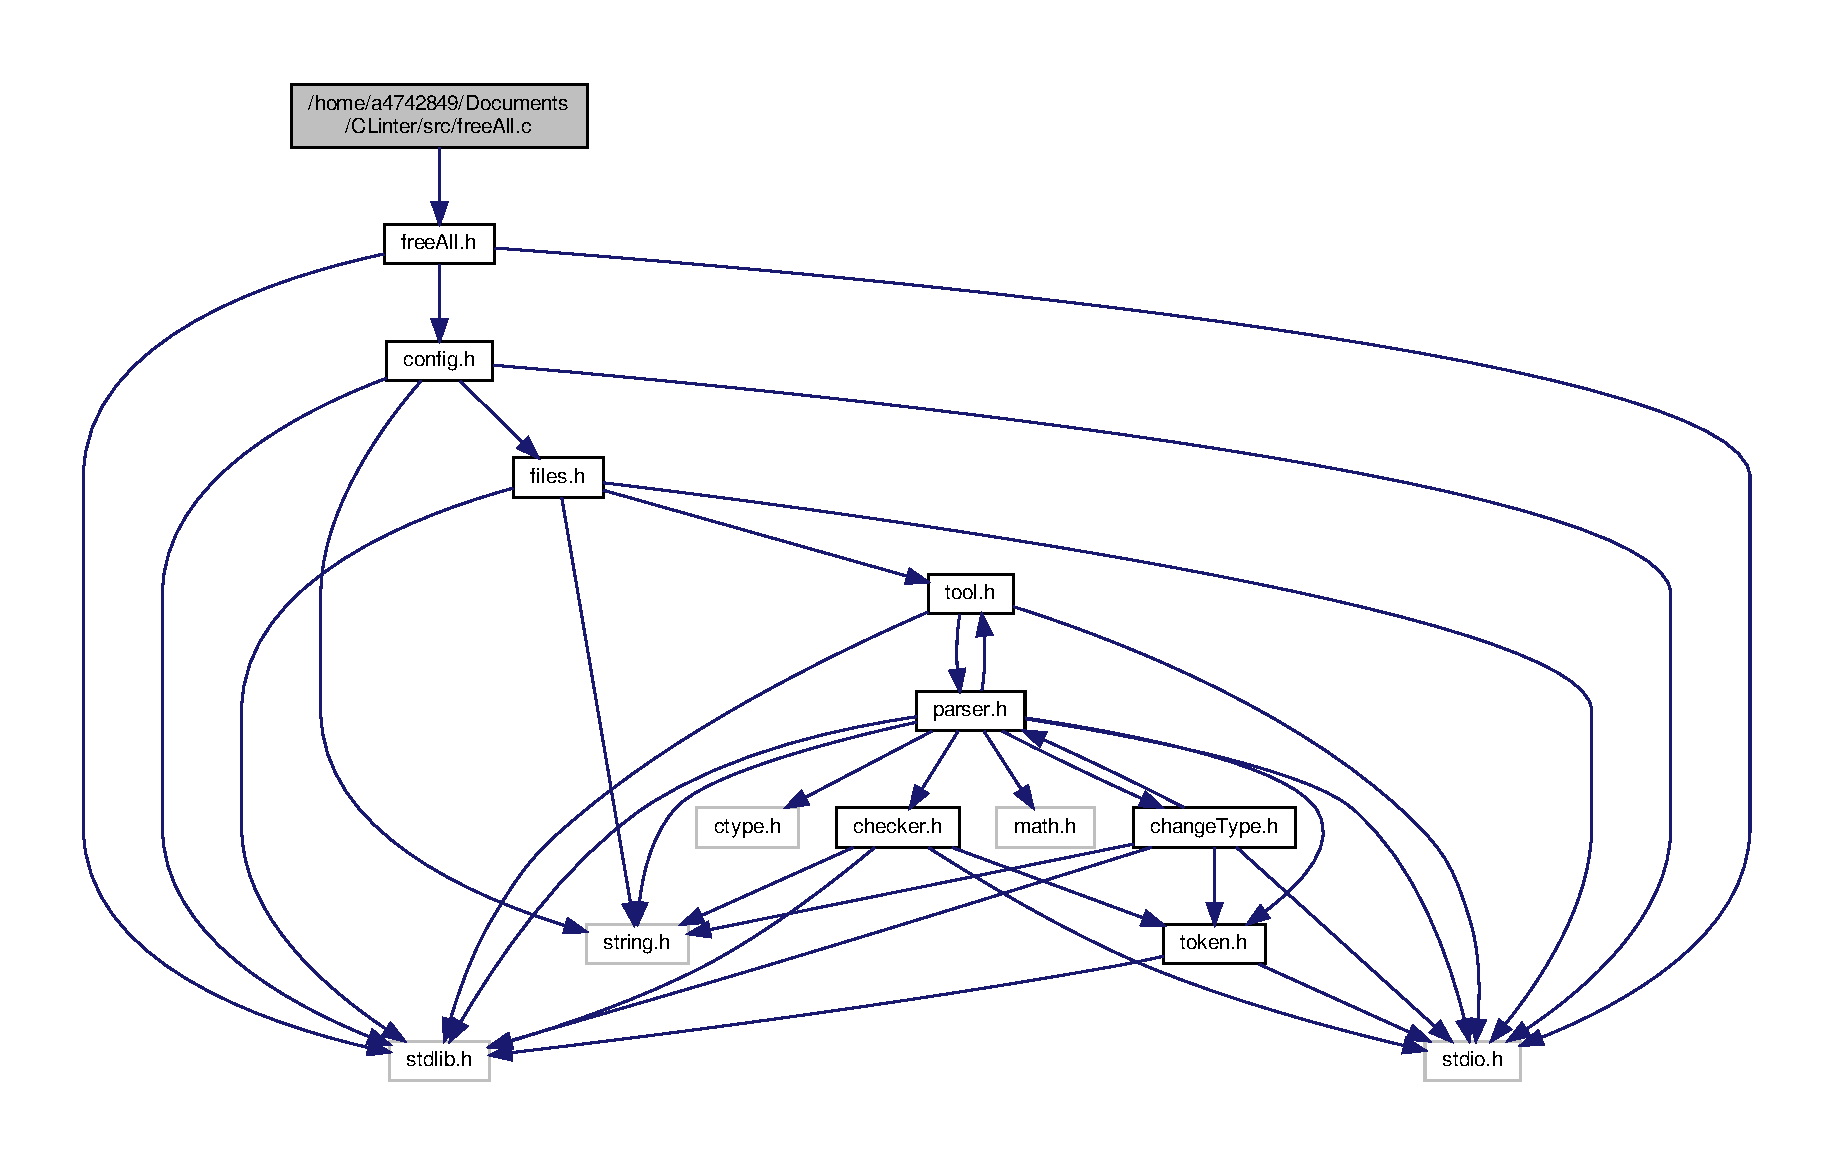
\includegraphics[width=350pt]{freeAll_8c__incl}
\end{center}
\end{figure}
\subsection*{Functions}
\begin{DoxyCompactItemize}
\item 
void \hyperlink{freeAll_8c_adf6fc31353c677ab80cca1e6ebc1338a}{clean\+\_\+text} (char $\ast$$\ast$code\+Text, int nb\+Lines)
\begin{DoxyCompactList}\small\item\em Replace all characters by \textquotesingle{}\textbackslash{}0\textquotesingle{} in code\+Text to wipe all Data. \end{DoxyCompactList}\item 
void \hyperlink{freeAll_8c_a48c8296b40b719d2e70cde772ce23b17}{free\+\_\+files} (char $\ast$$\ast$files, int nb\+Files)
\begin{DoxyCompactList}\small\item\em Free list of files (string). Similar has free\+\_\+text. \end{DoxyCompactList}\item 
void \hyperlink{freeAll_8c_ac06b54d9193690dc96e12efd015fda79}{free\+\_\+token\+List} (\hyperlink{token_8h_af79b1a4f53ad41cc0de4b364b9455dba}{Token} $\ast$$\ast$token\+List, int nb\+Nodes)
\begin{DoxyCompactList}\small\item\em Free content of a list of Tokens. \end{DoxyCompactList}\item 
void \hyperlink{freeAll_8c_a829139533619a6370dd21489c180fa03}{free\+\_\+text} (char $\ast$$\ast$code\+Text, int nb\+Lines)
\begin{DoxyCompactList}\small\item\em Free code Text. \end{DoxyCompactList}\item 
void \hyperlink{freeAll_8c_aa4996ba9c4a433b152f9550cc6949a98}{free\+\_\+conf} (\hyperlink{config_8h_a88ebb5d72d9993f342c6a9ae222a743c}{Config} $\ast$conf)
\begin{DoxyCompactList}\small\item\em Free the configuration structure. \end{DoxyCompactList}\end{DoxyCompactItemize}


\subsection{Detailed Description}
This c file will contain all functions to free all structures and pointers. 

\begin{DoxyAuthor}{Author}
Antoine T\+A\+V\+E\+R\+N\+I\+ER
\end{DoxyAuthor}
\begin{DoxyDate}{Date}
16/11/2018 
\end{DoxyDate}


\subsection{Function Documentation}
\mbox{\Hypertarget{freeAll_8c_adf6fc31353c677ab80cca1e6ebc1338a}\label{freeAll_8c_adf6fc31353c677ab80cca1e6ebc1338a}} 
\index{free\+All.\+c@{free\+All.\+c}!clean\+\_\+text@{clean\+\_\+text}}
\index{clean\+\_\+text@{clean\+\_\+text}!free\+All.\+c@{free\+All.\+c}}
\subsubsection{\texorpdfstring{clean\+\_\+text()}{clean\_text()}}
{\footnotesize\ttfamily void clean\+\_\+text (\begin{DoxyParamCaption}\item[{char $\ast$$\ast$}]{code\+Text,  }\item[{int}]{nb\+Lines }\end{DoxyParamCaption})}



Replace all characters by \textquotesingle{}\textbackslash{}0\textquotesingle{} in code\+Text to wipe all Data. 


\begin{DoxyParams}{Parameters}
{\em code\+Text} & A list of string \\
\hline
{\em nb\+Lines} & Number of strings in the list \\
\hline
\end{DoxyParams}
\mbox{\Hypertarget{freeAll_8c_aa4996ba9c4a433b152f9550cc6949a98}\label{freeAll_8c_aa4996ba9c4a433b152f9550cc6949a98}} 
\index{free\+All.\+c@{free\+All.\+c}!free\+\_\+conf@{free\+\_\+conf}}
\index{free\+\_\+conf@{free\+\_\+conf}!free\+All.\+c@{free\+All.\+c}}
\subsubsection{\texorpdfstring{free\+\_\+conf()}{free\_conf()}}
{\footnotesize\ttfamily void free\+\_\+conf (\begin{DoxyParamCaption}\item[{\hyperlink{config_8h_a88ebb5d72d9993f342c6a9ae222a743c}{Config} $\ast$}]{conf }\end{DoxyParamCaption})}



Free the configuration structure. 


\begin{DoxyParams}{Parameters}
{\em conf} & Config structure \\
\hline
\end{DoxyParams}
\mbox{\Hypertarget{freeAll_8c_a48c8296b40b719d2e70cde772ce23b17}\label{freeAll_8c_a48c8296b40b719d2e70cde772ce23b17}} 
\index{free\+All.\+c@{free\+All.\+c}!free\+\_\+files@{free\+\_\+files}}
\index{free\+\_\+files@{free\+\_\+files}!free\+All.\+c@{free\+All.\+c}}
\subsubsection{\texorpdfstring{free\+\_\+files()}{free\_files()}}
{\footnotesize\ttfamily void free\+\_\+files (\begin{DoxyParamCaption}\item[{char $\ast$$\ast$}]{files,  }\item[{int}]{nb\+Files }\end{DoxyParamCaption})}



Free list of files (string). Similar has free\+\_\+text. 


\begin{DoxyParams}{Parameters}
{\em files} & List of files \\
\hline
{\em nb\+Files} & Number of files in the list \\
\hline
\end{DoxyParams}
\mbox{\Hypertarget{freeAll_8c_a829139533619a6370dd21489c180fa03}\label{freeAll_8c_a829139533619a6370dd21489c180fa03}} 
\index{free\+All.\+c@{free\+All.\+c}!free\+\_\+text@{free\+\_\+text}}
\index{free\+\_\+text@{free\+\_\+text}!free\+All.\+c@{free\+All.\+c}}
\subsubsection{\texorpdfstring{free\+\_\+text()}{free\_text()}}
{\footnotesize\ttfamily void free\+\_\+text (\begin{DoxyParamCaption}\item[{char $\ast$$\ast$}]{code\+Text,  }\item[{int}]{nb\+Lines }\end{DoxyParamCaption})}



Free code Text. 


\begin{DoxyParams}{Parameters}
{\em code\+Text} & A list of string \\
\hline
{\em nb\+Lines} & Number of strings in the list \\
\hline
\end{DoxyParams}
\mbox{\Hypertarget{freeAll_8c_ac06b54d9193690dc96e12efd015fda79}\label{freeAll_8c_ac06b54d9193690dc96e12efd015fda79}} 
\index{free\+All.\+c@{free\+All.\+c}!free\+\_\+token\+List@{free\+\_\+token\+List}}
\index{free\+\_\+token\+List@{free\+\_\+token\+List}!free\+All.\+c@{free\+All.\+c}}
\subsubsection{\texorpdfstring{free\+\_\+token\+List()}{free\_tokenList()}}
{\footnotesize\ttfamily void free\+\_\+token\+List (\begin{DoxyParamCaption}\item[{\hyperlink{token_8h_af79b1a4f53ad41cc0de4b364b9455dba}{Token} $\ast$$\ast$}]{token\+List,  }\item[{int}]{nb\+Nodes }\end{DoxyParamCaption})}



Free content of a list of Tokens. 


\begin{DoxyParams}{Parameters}
{\em token\+List} & List of Tokens to free \\
\hline
{\em nb\+Nodes} & Numbers of Tokens in the list \\
\hline
\end{DoxyParams}

\hypertarget{freeAll_8h}{}\section{/home/a4742849/\+Documents/\+C\+Linter/src/free\+All.h File Reference}
\label{freeAll_8h}\index{/home/a4742849/\+Documents/\+C\+Linter/src/free\+All.\+h@{/home/a4742849/\+Documents/\+C\+Linter/src/free\+All.\+h}}


This header file will contain all required definitions and basic utilities functions to free the memory of the program.  


{\ttfamily \#include $<$stdlib.\+h$>$}\newline
{\ttfamily \#include $<$stdio.\+h$>$}\newline
{\ttfamily \#include \char`\"{}config.\+h\char`\"{}}\newline
Include dependency graph for free\+All.\+h\+:\nopagebreak
\begin{figure}[H]
\begin{center}
\leavevmode
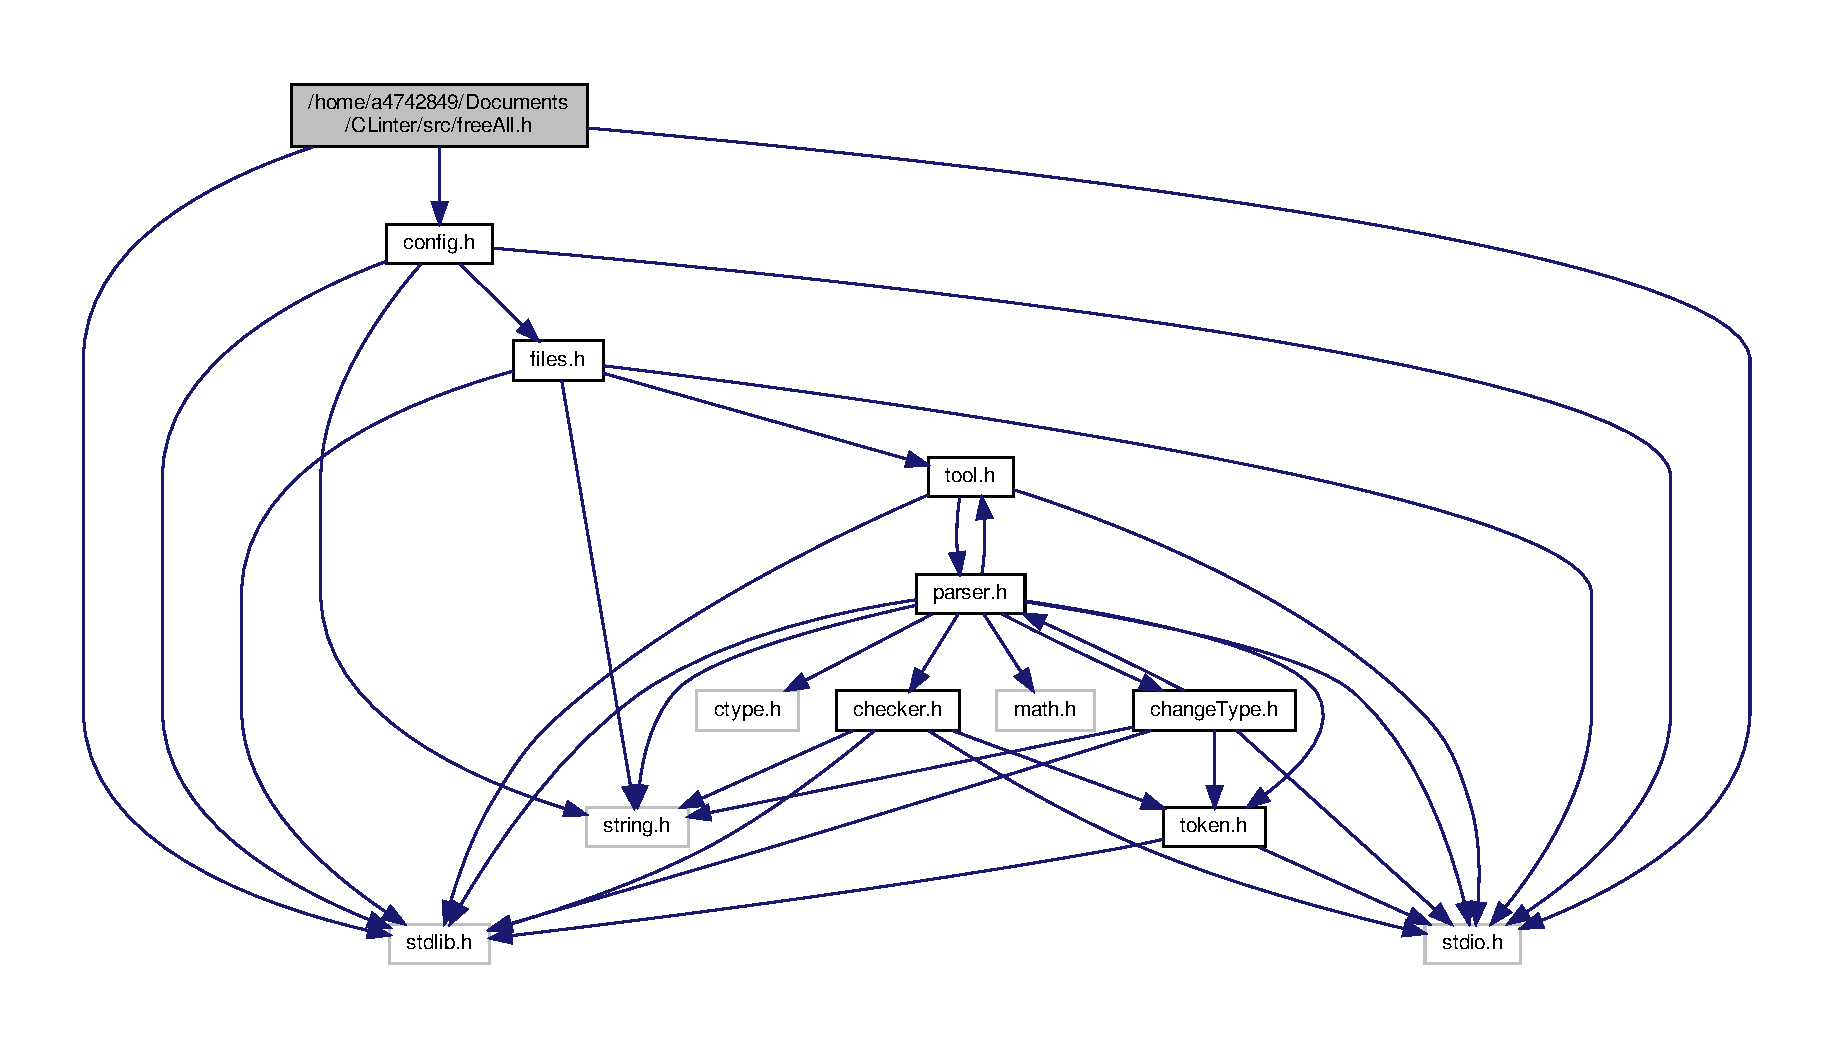
\includegraphics[width=350pt]{freeAll_8h__incl}
\end{center}
\end{figure}
This graph shows which files directly or indirectly include this file\+:
\nopagebreak
\begin{figure}[H]
\begin{center}
\leavevmode
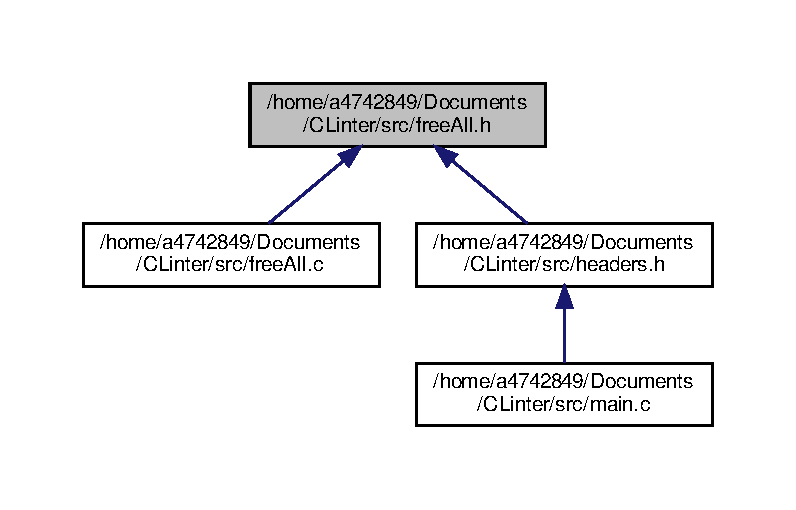
\includegraphics[width=350pt]{freeAll_8h__dep__incl}
\end{center}
\end{figure}
\subsection*{Functions}
\begin{DoxyCompactItemize}
\item 
void \hyperlink{freeAll_8h_adf6fc31353c677ab80cca1e6ebc1338a}{clean\+\_\+text} (char $\ast$$\ast$code\+Text, int nb\+Lines)
\begin{DoxyCompactList}\small\item\em Replace all characters by \textquotesingle{}\textbackslash{}0\textquotesingle{} in code\+Text to wipe all Data. \end{DoxyCompactList}\item 
void \hyperlink{freeAll_8h_aa4996ba9c4a433b152f9550cc6949a98}{free\+\_\+conf} (\hyperlink{config_8h_a88ebb5d72d9993f342c6a9ae222a743c}{Config} $\ast$conf)
\begin{DoxyCompactList}\small\item\em Free the configuration structure. \end{DoxyCompactList}\item 
void \hyperlink{freeAll_8h_a829139533619a6370dd21489c180fa03}{free\+\_\+text} (char $\ast$$\ast$code\+Text, int nb\+Lines)
\begin{DoxyCompactList}\small\item\em Free code Text. \end{DoxyCompactList}\item 
void \hyperlink{freeAll_8h_ac06b54d9193690dc96e12efd015fda79}{free\+\_\+token\+List} (\hyperlink{token_8h_af79b1a4f53ad41cc0de4b364b9455dba}{Token} $\ast$$\ast$token\+List, int nb\+Nodes)
\begin{DoxyCompactList}\small\item\em Free content of a list of Tokens. \end{DoxyCompactList}\item 
void \hyperlink{freeAll_8h_a48c8296b40b719d2e70cde772ce23b17}{free\+\_\+files} (char $\ast$$\ast$files, int nb\+Files)
\begin{DoxyCompactList}\small\item\em Free list of files (string). Similar has free\+\_\+text. \end{DoxyCompactList}\end{DoxyCompactItemize}


\subsection{Detailed Description}
This header file will contain all required definitions and basic utilities functions to free the memory of the program. 

\begin{DoxyAuthor}{Author}
Antoine T\+A\+V\+E\+R\+N\+I\+ER
\end{DoxyAuthor}
\begin{DoxyDate}{Date}
16/11/2018 
\end{DoxyDate}


\subsection{Function Documentation}
\mbox{\Hypertarget{freeAll_8h_adf6fc31353c677ab80cca1e6ebc1338a}\label{freeAll_8h_adf6fc31353c677ab80cca1e6ebc1338a}} 
\index{free\+All.\+h@{free\+All.\+h}!clean\+\_\+text@{clean\+\_\+text}}
\index{clean\+\_\+text@{clean\+\_\+text}!free\+All.\+h@{free\+All.\+h}}
\subsubsection{\texorpdfstring{clean\+\_\+text()}{clean\_text()}}
{\footnotesize\ttfamily void clean\+\_\+text (\begin{DoxyParamCaption}\item[{char $\ast$$\ast$}]{code\+Text,  }\item[{int}]{nb\+Lines }\end{DoxyParamCaption})}



Replace all characters by \textquotesingle{}\textbackslash{}0\textquotesingle{} in code\+Text to wipe all Data. 


\begin{DoxyParams}{Parameters}
{\em code\+Text} & A list of string \\
\hline
{\em nb\+Lines} & Number of strings in the list \\
\hline
\end{DoxyParams}
\mbox{\Hypertarget{freeAll_8h_aa4996ba9c4a433b152f9550cc6949a98}\label{freeAll_8h_aa4996ba9c4a433b152f9550cc6949a98}} 
\index{free\+All.\+h@{free\+All.\+h}!free\+\_\+conf@{free\+\_\+conf}}
\index{free\+\_\+conf@{free\+\_\+conf}!free\+All.\+h@{free\+All.\+h}}
\subsubsection{\texorpdfstring{free\+\_\+conf()}{free\_conf()}}
{\footnotesize\ttfamily void free\+\_\+conf (\begin{DoxyParamCaption}\item[{\hyperlink{config_8h_a88ebb5d72d9993f342c6a9ae222a743c}{Config} $\ast$}]{conf }\end{DoxyParamCaption})}



Free the configuration structure. 


\begin{DoxyParams}{Parameters}
{\em conf} & Config structure \\
\hline
\end{DoxyParams}
\mbox{\Hypertarget{freeAll_8h_a48c8296b40b719d2e70cde772ce23b17}\label{freeAll_8h_a48c8296b40b719d2e70cde772ce23b17}} 
\index{free\+All.\+h@{free\+All.\+h}!free\+\_\+files@{free\+\_\+files}}
\index{free\+\_\+files@{free\+\_\+files}!free\+All.\+h@{free\+All.\+h}}
\subsubsection{\texorpdfstring{free\+\_\+files()}{free\_files()}}
{\footnotesize\ttfamily void free\+\_\+files (\begin{DoxyParamCaption}\item[{char $\ast$$\ast$}]{files,  }\item[{int}]{nb\+Files }\end{DoxyParamCaption})}



Free list of files (string). Similar has free\+\_\+text. 


\begin{DoxyParams}{Parameters}
{\em files} & List of files \\
\hline
{\em nb\+Files} & Number of files in the list \\
\hline
\end{DoxyParams}
\mbox{\Hypertarget{freeAll_8h_a829139533619a6370dd21489c180fa03}\label{freeAll_8h_a829139533619a6370dd21489c180fa03}} 
\index{free\+All.\+h@{free\+All.\+h}!free\+\_\+text@{free\+\_\+text}}
\index{free\+\_\+text@{free\+\_\+text}!free\+All.\+h@{free\+All.\+h}}
\subsubsection{\texorpdfstring{free\+\_\+text()}{free\_text()}}
{\footnotesize\ttfamily void free\+\_\+text (\begin{DoxyParamCaption}\item[{char $\ast$$\ast$}]{code\+Text,  }\item[{int}]{nb\+Lines }\end{DoxyParamCaption})}



Free code Text. 


\begin{DoxyParams}{Parameters}
{\em code\+Text} & A list of string \\
\hline
{\em nb\+Lines} & Number of strings in the list \\
\hline
\end{DoxyParams}
\mbox{\Hypertarget{freeAll_8h_ac06b54d9193690dc96e12efd015fda79}\label{freeAll_8h_ac06b54d9193690dc96e12efd015fda79}} 
\index{free\+All.\+h@{free\+All.\+h}!free\+\_\+token\+List@{free\+\_\+token\+List}}
\index{free\+\_\+token\+List@{free\+\_\+token\+List}!free\+All.\+h@{free\+All.\+h}}
\subsubsection{\texorpdfstring{free\+\_\+token\+List()}{free\_tokenList()}}
{\footnotesize\ttfamily void free\+\_\+token\+List (\begin{DoxyParamCaption}\item[{\hyperlink{token_8h_af79b1a4f53ad41cc0de4b364b9455dba}{Token} $\ast$$\ast$}]{token\+List,  }\item[{int}]{nb\+Nodes }\end{DoxyParamCaption})}



Free content of a list of Tokens. 


\begin{DoxyParams}{Parameters}
{\em token\+List} & List of Tokens to free \\
\hline
{\em nb\+Nodes} & Numbers of Tokens in the list \\
\hline
\end{DoxyParams}

\hypertarget{headers_8h}{}\section{/home/a4742849/\+Documents/\+C\+Linter/src/headers.h File Reference}
\label{headers_8h}\index{/home/a4742849/\+Documents/\+C\+Linter/src/headers.\+h@{/home/a4742849/\+Documents/\+C\+Linter/src/headers.\+h}}


This header file will contain all required definitions and basic header files for main function.  


{\ttfamily \#include $<$stdlib.\+h$>$}\newline
{\ttfamily \#include $<$stdio.\+h$>$}\newline
{\ttfamily \#include $<$string.\+h$>$}\newline
{\ttfamily \#include \char`\"{}change\+Type.\+h\char`\"{}}\newline
{\ttfamily \#include \char`\"{}tool.\+h\char`\"{}}\newline
{\ttfamily \#include \char`\"{}parser.\+h\char`\"{}}\newline
{\ttfamily \#include \char`\"{}files.\+h\char`\"{}}\newline
{\ttfamily \#include \char`\"{}token.\+h\char`\"{}}\newline
{\ttfamily \#include \char`\"{}config.\+h\char`\"{}}\newline
{\ttfamily \#include \char`\"{}check\+Coding.\+h\char`\"{}}\newline
{\ttfamily \#include \char`\"{}check\+Var\+Func.\+h\char`\"{}}\newline
{\ttfamily \#include \char`\"{}list\+Files.\+h\char`\"{}}\newline
{\ttfamily \#include \char`\"{}free\+All.\+h\char`\"{}}\newline
Include dependency graph for headers.\+h\+:\nopagebreak
\begin{figure}[H]
\begin{center}
\leavevmode
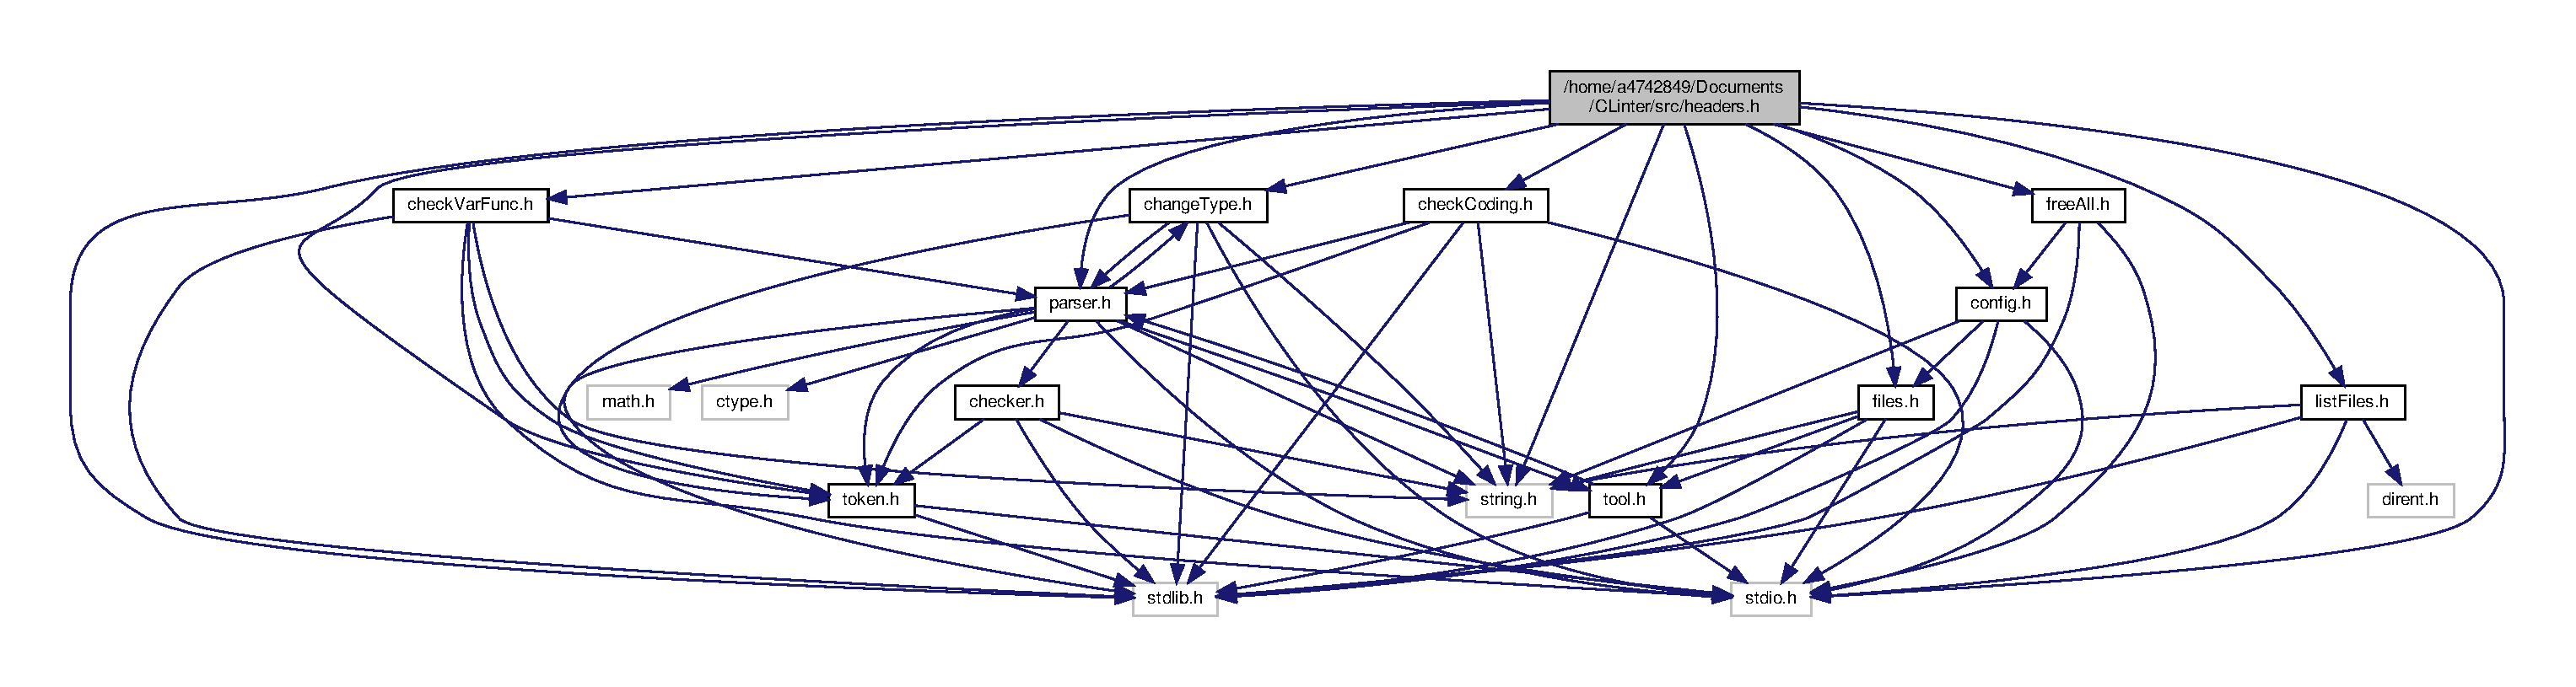
\includegraphics[width=350pt]{headers_8h__incl}
\end{center}
\end{figure}
This graph shows which files directly or indirectly include this file\+:
\nopagebreak
\begin{figure}[H]
\begin{center}
\leavevmode
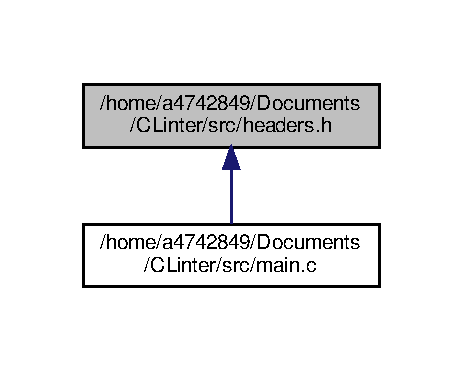
\includegraphics[width=222pt]{headers_8h__dep__incl}
\end{center}
\end{figure}


\subsection{Detailed Description}
This header file will contain all required definitions and basic header files for main function. 

\begin{DoxyAuthor}{Author}
Antoine T\+A\+V\+E\+R\+N\+I\+ER
\end{DoxyAuthor}
\begin{DoxyDate}{Date}
16/11/2018 
\end{DoxyDate}

\hypertarget{listFiles_8c}{}\section{/home/a4742849/\+Documents/\+C\+Linter/src/list\+Files.c File Reference}
\label{listFiles_8c}\index{/home/a4742849/\+Documents/\+C\+Linter/src/list\+Files.\+c@{/home/a4742849/\+Documents/\+C\+Linter/src/list\+Files.\+c}}


This c file will contain all functions to list files we want to work on.  


{\ttfamily \#include \char`\"{}list\+Files.\+h\char`\"{}}\newline
Include dependency graph for list\+Files.\+c\+:\nopagebreak
\begin{figure}[H]
\begin{center}
\leavevmode
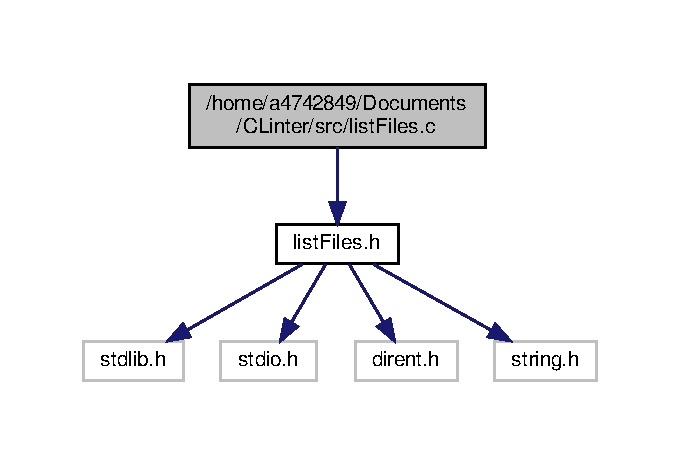
\includegraphics[width=327pt]{listFiles_8c__incl}
\end{center}
\end{figure}
\subsection*{Functions}
\begin{DoxyCompactItemize}
\item 
int \hyperlink{listFiles_8c_a0c74c65f13b3f9f5870909701fdc33b1}{is\+Not\+Excluded} (char $\ast$$\ast$excluded\+Files, char $\ast$file, int length)
\begin{DoxyCompactList}\small\item\em Check if a given file is not in the list of excluded files from config. \end{DoxyCompactList}\item 
void \hyperlink{listFiles_8c_a0a47e47fbbdee433b7f4da7b3d57b288}{get\+Files} (char $\ast$$\ast$files, int $\ast$pos, short is\+Recursive, char $\ast$$\ast$excluded\+Files, char $\ast$path, int length)
\begin{DoxyCompactList}\small\item\em Get the Files from list a path. \end{DoxyCompactList}\end{DoxyCompactItemize}


\subsection{Detailed Description}
This c file will contain all functions to list files we want to work on. 

\begin{DoxyAuthor}{Author}
Antoine T\+A\+V\+E\+R\+N\+I\+ER
\end{DoxyAuthor}
\begin{DoxyDate}{Date}
16/11/2018 
\end{DoxyDate}


\subsection{Function Documentation}
\mbox{\Hypertarget{listFiles_8c_a0a47e47fbbdee433b7f4da7b3d57b288}\label{listFiles_8c_a0a47e47fbbdee433b7f4da7b3d57b288}} 
\index{list\+Files.\+c@{list\+Files.\+c}!get\+Files@{get\+Files}}
\index{get\+Files@{get\+Files}!list\+Files.\+c@{list\+Files.\+c}}
\subsubsection{\texorpdfstring{get\+Files()}{getFiles()}}
{\footnotesize\ttfamily void get\+Files (\begin{DoxyParamCaption}\item[{char $\ast$$\ast$}]{files,  }\item[{int $\ast$}]{pos,  }\item[{short}]{is\+Recursive,  }\item[{char $\ast$$\ast$}]{excluded\+Files,  }\item[{char $\ast$}]{path,  }\item[{int}]{length }\end{DoxyParamCaption})}



Get the Files from list a path. 


\begin{DoxyParams}{Parameters}
{\em files} & A list of File names \\
\hline
{\em pos} & Position in the list of File names \\
\hline
{\em is\+Recursive} & 0 false else true \\
\hline
{\em excluded\+Files} & List of excluded files \\
\hline
{\em path} & Path of the file \\
\hline
{\em length} & Number of excluded files \\
\hline
\end{DoxyParams}
\mbox{\Hypertarget{listFiles_8c_a0c74c65f13b3f9f5870909701fdc33b1}\label{listFiles_8c_a0c74c65f13b3f9f5870909701fdc33b1}} 
\index{list\+Files.\+c@{list\+Files.\+c}!is\+Not\+Excluded@{is\+Not\+Excluded}}
\index{is\+Not\+Excluded@{is\+Not\+Excluded}!list\+Files.\+c@{list\+Files.\+c}}
\subsubsection{\texorpdfstring{is\+Not\+Excluded()}{isNotExcluded()}}
{\footnotesize\ttfamily int is\+Not\+Excluded (\begin{DoxyParamCaption}\item[{char $\ast$$\ast$}]{excluded\+Files,  }\item[{char $\ast$}]{file,  }\item[{int}]{length }\end{DoxyParamCaption})}



Check if a given file is not in the list of excluded files from config. 


\begin{DoxyParams}{Parameters}
{\em excluded\+Files} & List of excluded files \\
\hline
{\em file} & The given file to check \\
\hline
{\em length} & Number of exlucded files in the list \\
\hline
\end{DoxyParams}
\begin{DoxyReturn}{Returns}
int 0 false else true 
\end{DoxyReturn}

\hypertarget{listFiles_8h}{}\section{/home/a4742849/\+Documents/\+C\+Linter/src/list\+Files.h File Reference}
\label{listFiles_8h}\index{/home/a4742849/\+Documents/\+C\+Linter/src/list\+Files.\+h@{/home/a4742849/\+Documents/\+C\+Linter/src/list\+Files.\+h}}


This header file will contain all required definitions and basic utilities functions to check grammar of a C file.  


{\ttfamily \#include $<$stdlib.\+h$>$}\newline
{\ttfamily \#include $<$stdio.\+h$>$}\newline
{\ttfamily \#include $<$dirent.\+h$>$}\newline
{\ttfamily \#include $<$string.\+h$>$}\newline
Include dependency graph for list\+Files.\+h\+:\nopagebreak
\begin{figure}[H]
\begin{center}
\leavevmode
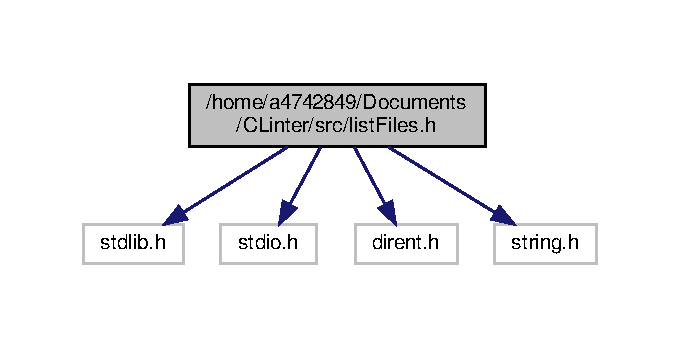
\includegraphics[width=327pt]{listFiles_8h__incl}
\end{center}
\end{figure}
This graph shows which files directly or indirectly include this file\+:
\nopagebreak
\begin{figure}[H]
\begin{center}
\leavevmode
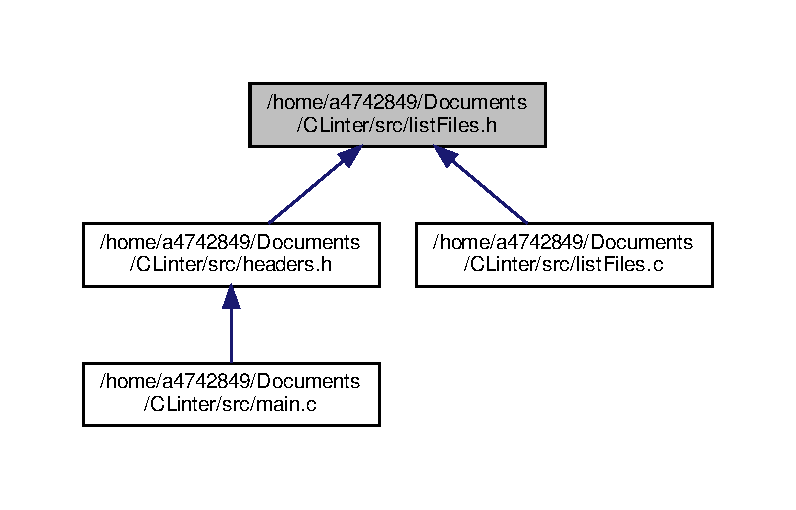
\includegraphics[width=350pt]{listFiles_8h__dep__incl}
\end{center}
\end{figure}
\subsection*{Macros}
\begin{DoxyCompactItemize}
\item 
\#define \hyperlink{listFiles_8h_a369266c24eacffb87046522897a570d5}{\+\_\+\+G\+N\+U\+\_\+\+S\+O\+U\+R\+CE}
\end{DoxyCompactItemize}
\subsection*{Functions}
\begin{DoxyCompactItemize}
\item 
int \hyperlink{listFiles_8h_a0c74c65f13b3f9f5870909701fdc33b1}{is\+Not\+Excluded} (char $\ast$$\ast$excluded\+Files, char $\ast$file, int length)
\begin{DoxyCompactList}\small\item\em Check if a given file is not in the list of excluded files from config. \end{DoxyCompactList}\item 
void \hyperlink{listFiles_8h_a0a47e47fbbdee433b7f4da7b3d57b288}{get\+Files} (char $\ast$$\ast$files, int $\ast$pos, short is\+Recursive, char $\ast$$\ast$excluded\+Files, char $\ast$path, int length)
\begin{DoxyCompactList}\small\item\em Get the Files from list a path. \end{DoxyCompactList}\end{DoxyCompactItemize}


\subsection{Detailed Description}
This header file will contain all required definitions and basic utilities functions to check grammar of a C file. 

\begin{DoxyAuthor}{Author}
Antoine T\+A\+V\+E\+R\+N\+I\+ER
\end{DoxyAuthor}
\begin{DoxyDate}{Date}
16/11/2018 
\end{DoxyDate}


\subsection{Macro Definition Documentation}
\mbox{\Hypertarget{listFiles_8h_a369266c24eacffb87046522897a570d5}\label{listFiles_8h_a369266c24eacffb87046522897a570d5}} 
\index{list\+Files.\+h@{list\+Files.\+h}!\+\_\+\+G\+N\+U\+\_\+\+S\+O\+U\+R\+CE@{\+\_\+\+G\+N\+U\+\_\+\+S\+O\+U\+R\+CE}}
\index{\+\_\+\+G\+N\+U\+\_\+\+S\+O\+U\+R\+CE@{\+\_\+\+G\+N\+U\+\_\+\+S\+O\+U\+R\+CE}!list\+Files.\+h@{list\+Files.\+h}}
\subsubsection{\texorpdfstring{\+\_\+\+G\+N\+U\+\_\+\+S\+O\+U\+R\+CE}{\_GNU\_SOURCE}}
{\footnotesize\ttfamily \#define \+\_\+\+G\+N\+U\+\_\+\+S\+O\+U\+R\+CE}



\subsection{Function Documentation}
\mbox{\Hypertarget{listFiles_8h_a0a47e47fbbdee433b7f4da7b3d57b288}\label{listFiles_8h_a0a47e47fbbdee433b7f4da7b3d57b288}} 
\index{list\+Files.\+h@{list\+Files.\+h}!get\+Files@{get\+Files}}
\index{get\+Files@{get\+Files}!list\+Files.\+h@{list\+Files.\+h}}
\subsubsection{\texorpdfstring{get\+Files()}{getFiles()}}
{\footnotesize\ttfamily void get\+Files (\begin{DoxyParamCaption}\item[{char $\ast$$\ast$}]{files,  }\item[{int $\ast$}]{pos,  }\item[{short}]{is\+Recursive,  }\item[{char $\ast$$\ast$}]{excluded\+Files,  }\item[{char $\ast$}]{path,  }\item[{int}]{length }\end{DoxyParamCaption})}



Get the Files from list a path. 


\begin{DoxyParams}{Parameters}
{\em files} & A list of File names \\
\hline
{\em pos} & Position in the list of File names \\
\hline
{\em is\+Recursive} & 0 false else true \\
\hline
{\em excluded\+Files} & List of excluded files \\
\hline
{\em path} & Path of the file \\
\hline
{\em length} & Number of excluded files \\
\hline
\end{DoxyParams}
\mbox{\Hypertarget{listFiles_8h_a0c74c65f13b3f9f5870909701fdc33b1}\label{listFiles_8h_a0c74c65f13b3f9f5870909701fdc33b1}} 
\index{list\+Files.\+h@{list\+Files.\+h}!is\+Not\+Excluded@{is\+Not\+Excluded}}
\index{is\+Not\+Excluded@{is\+Not\+Excluded}!list\+Files.\+h@{list\+Files.\+h}}
\subsubsection{\texorpdfstring{is\+Not\+Excluded()}{isNotExcluded()}}
{\footnotesize\ttfamily int is\+Not\+Excluded (\begin{DoxyParamCaption}\item[{char $\ast$$\ast$}]{excluded\+Files,  }\item[{char $\ast$}]{file,  }\item[{int}]{length }\end{DoxyParamCaption})}



Check if a given file is not in the list of excluded files from config. 


\begin{DoxyParams}{Parameters}
{\em excluded\+Files} & List of excluded files \\
\hline
{\em file} & The given file to check \\
\hline
{\em length} & Number of exlucded files in the list \\
\hline
\end{DoxyParams}
\begin{DoxyReturn}{Returns}
int 0 false else true 
\end{DoxyReturn}

\hypertarget{main_8c}{}\section{/home/a4742849/\+Documents/\+C\+Linter/src/main.c File Reference}
\label{main_8c}\index{/home/a4742849/\+Documents/\+C\+Linter/src/main.\+c@{/home/a4742849/\+Documents/\+C\+Linter/src/main.\+c}}


This c file will contain all the logic to analyze and warn a user of it\textquotesingle{}s bad C type skills.  


{\ttfamily \#include \char`\"{}headers.\+h\char`\"{}}\newline
Include dependency graph for main.\+c\+:\nopagebreak
\begin{figure}[H]
\begin{center}
\leavevmode
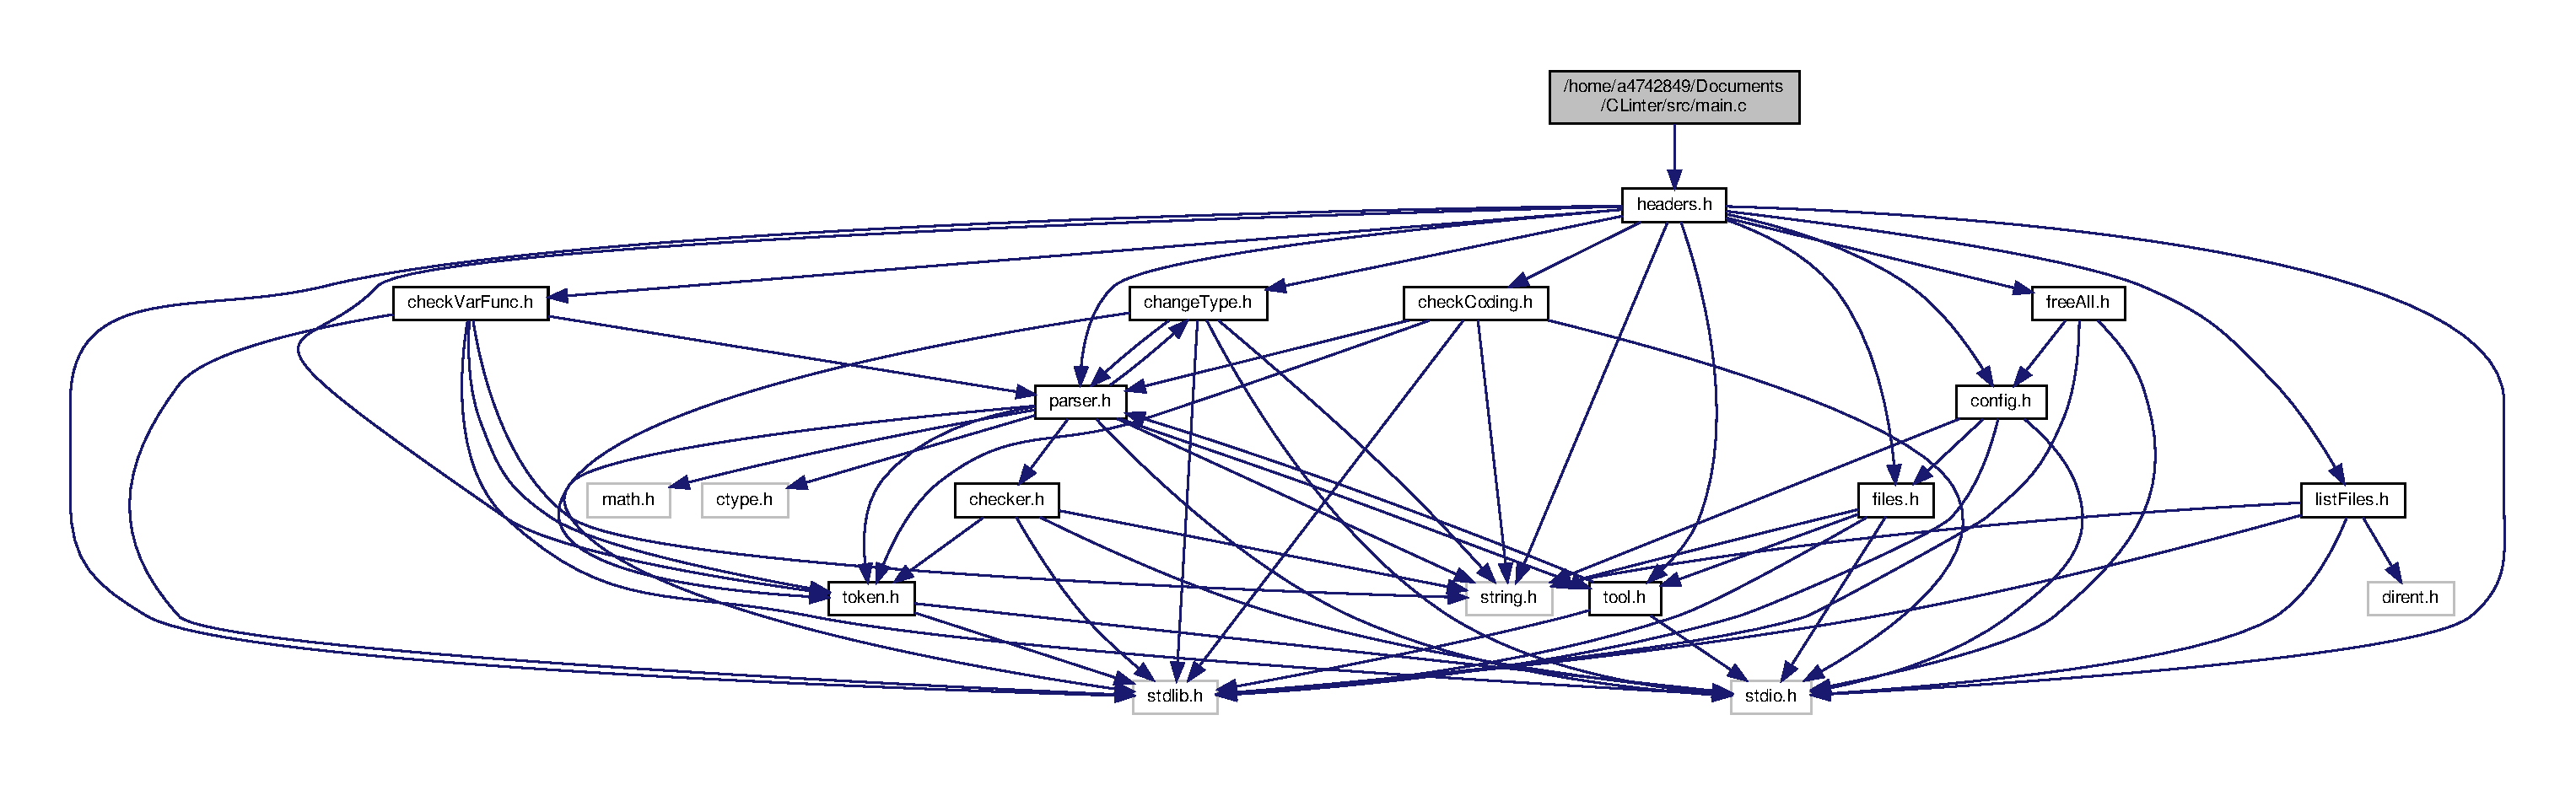
\includegraphics[width=350pt]{main_8c__incl}
\end{center}
\end{figure}
\subsection*{Functions}
\begin{DoxyCompactItemize}
\item 
int \hyperlink{main_8c_a0ddf1224851353fc92bfbff6f499fa97}{main} (int argc, char $\ast$argv\mbox{[}$\,$\mbox{]})
\begin{DoxyCompactList}\small\item\em The main entrance point of the program containing all the Logic. \end{DoxyCompactList}\end{DoxyCompactItemize}


\subsection{Detailed Description}
This c file will contain all the logic to analyze and warn a user of it\textquotesingle{}s bad C type skills. 

\begin{DoxyAuthor}{Author}
Antoine T\+A\+V\+E\+R\+N\+I\+ER
\end{DoxyAuthor}
\begin{DoxyDate}{Date}
16/11/2018 
\end{DoxyDate}


\subsection{Function Documentation}
\mbox{\Hypertarget{main_8c_a0ddf1224851353fc92bfbff6f499fa97}\label{main_8c_a0ddf1224851353fc92bfbff6f499fa97}} 
\index{main.\+c@{main.\+c}!main@{main}}
\index{main@{main}!main.\+c@{main.\+c}}
\subsubsection{\texorpdfstring{main()}{main()}}
{\footnotesize\ttfamily int main (\begin{DoxyParamCaption}\item[{int}]{argc,  }\item[{char $\ast$}]{argv\mbox{[}$\,$\mbox{]} }\end{DoxyParamCaption})}



The main entrance point of the program containing all the Logic. 


\begin{DoxyParams}{Parameters}
{\em argc} & Number of arguments \\
\hline
{\em argv} & List of arguments \\
\hline
\end{DoxyParams}
\begin{DoxyReturn}{Returns}
int 0 Good else Bad 
\end{DoxyReturn}

\hypertarget{parser_8c}{}\section{/home/a4742849/\+Documents/\+C\+Linter/src/parser.c File Reference}
\label{parser_8c}\index{/home/a4742849/\+Documents/\+C\+Linter/src/parser.\+c@{/home/a4742849/\+Documents/\+C\+Linter/src/parser.\+c}}


This c file will contain all functions to parse a file.  


{\ttfamily \#include \char`\"{}parser.\+h\char`\"{}}\newline
Include dependency graph for parser.\+c\+:\nopagebreak
\begin{figure}[H]
\begin{center}
\leavevmode
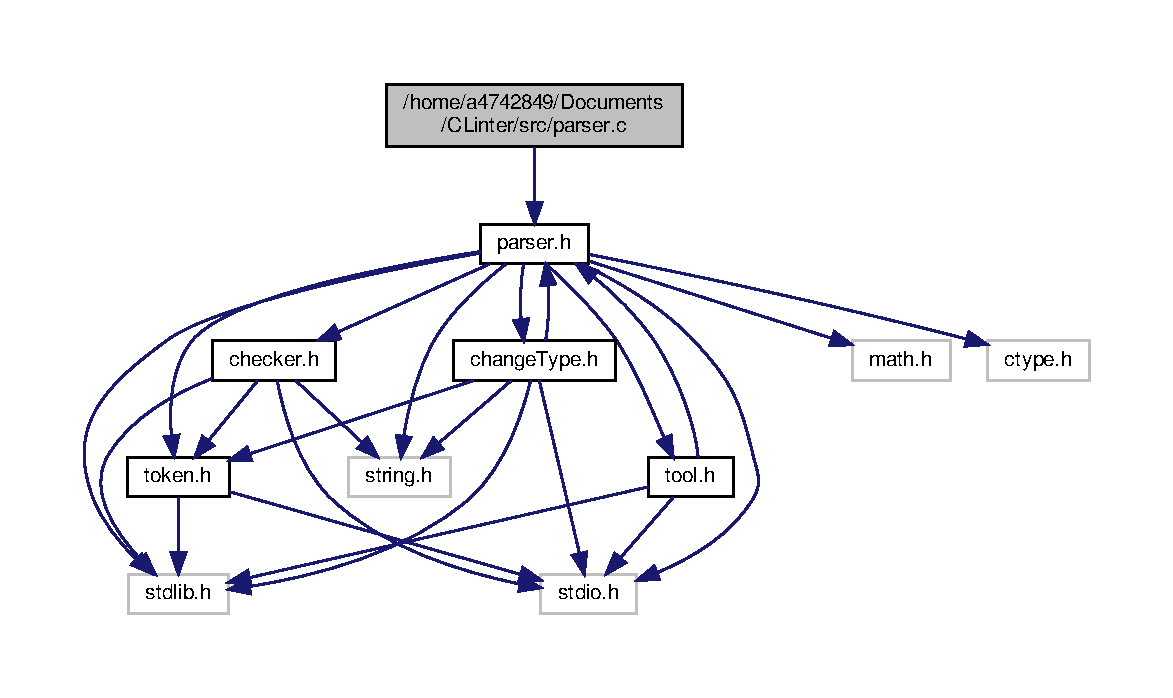
\includegraphics[width=350pt]{parser_8c__incl}
\end{center}
\end{figure}
\subsection*{Functions}
\begin{DoxyCompactItemize}
\item 
int \hyperlink{parser_8c_a32d638521fed670f56092d9220f17186}{is\+Ope} (char c)
\begin{DoxyCompactList}\small\item\em Tell if char is an operator. \end{DoxyCompactList}\item 
int \hyperlink{parser_8c_aa0c754508d5d35e6b7ca295174004323}{is\+Delim} (char c)
\begin{DoxyCompactList}\small\item\em Tell if char is a delimiter + operator. \end{DoxyCompactList}\item 
int \hyperlink{parser_8c_a5c8cb0c9a3afe1950d34267cfe898bc9}{is\+Delim\+No\+Space} (char c)
\begin{DoxyCompactList}\small\item\em Tell if char is a delimiter expect space \textquotesingle{} \textquotesingle{}. \end{DoxyCompactList}\item 
char $\ast$ \hyperlink{parser_8c_aa4859689aab814e043959441bf90f146}{get\+Sub\+String} (char $\ast$str, int left, int right)
\begin{DoxyCompactList}\small\item\em Get sub\+String of str delimited by left and right. \end{DoxyCompactList}\item 
int \hyperlink{parser_8c_ac948db34a6f84f0ae0fcc689e609ed62}{can\+Be\+Expe} (char c, char $\ast$str, int right)
\item 
\hyperlink{token_8h_af79b1a4f53ad41cc0de4b364b9455dba}{Token} $\ast$$\ast$ \hyperlink{parser_8c_adfdea08dc03111766b2a52dc0ffd9cb6}{parse} (char $\ast$str, int $\ast$nb\+Nodes)
\begin{DoxyCompactList}\small\item\em Reads a string and prints each token type. \end{DoxyCompactList}\end{DoxyCompactItemize}


\subsection{Detailed Description}
This c file will contain all functions to parse a file. 

\begin{DoxyAuthor}{Author}
Antoine T\+A\+V\+E\+R\+N\+I\+ER
\end{DoxyAuthor}
\begin{DoxyDate}{Date}
16/11/2018 
\end{DoxyDate}


\subsection{Function Documentation}
\mbox{\Hypertarget{parser_8c_ac948db34a6f84f0ae0fcc689e609ed62}\label{parser_8c_ac948db34a6f84f0ae0fcc689e609ed62}} 
\index{parser.\+c@{parser.\+c}!can\+Be\+Expe@{can\+Be\+Expe}}
\index{can\+Be\+Expe@{can\+Be\+Expe}!parser.\+c@{parser.\+c}}
\subsubsection{\texorpdfstring{can\+Be\+Expe()}{canBeExpe()}}
{\footnotesize\ttfamily int can\+Be\+Expe (\begin{DoxyParamCaption}\item[{char}]{c,  }\item[{char $\ast$}]{str,  }\item[{int}]{right }\end{DoxyParamCaption})}

\mbox{\Hypertarget{parser_8c_aa4859689aab814e043959441bf90f146}\label{parser_8c_aa4859689aab814e043959441bf90f146}} 
\index{parser.\+c@{parser.\+c}!get\+Sub\+String@{get\+Sub\+String}}
\index{get\+Sub\+String@{get\+Sub\+String}!parser.\+c@{parser.\+c}}
\subsubsection{\texorpdfstring{get\+Sub\+String()}{getSubString()}}
{\footnotesize\ttfamily char$\ast$ get\+Sub\+String (\begin{DoxyParamCaption}\item[{char $\ast$}]{str,  }\item[{int}]{left,  }\item[{int}]{right }\end{DoxyParamCaption})}



Get sub\+String of str delimited by left and right. 


\begin{DoxyParams}{Parameters}
{\em str} & String containing text \\
\hline
{\em left} & Left pointer on the str \\
\hline
{\em right} & Right pointer on the str \\
\hline
\end{DoxyParams}
\begin{DoxyReturn}{Returns}
char$\ast$ Substring between left and right pointers 
\end{DoxyReturn}
\mbox{\Hypertarget{parser_8c_aa0c754508d5d35e6b7ca295174004323}\label{parser_8c_aa0c754508d5d35e6b7ca295174004323}} 
\index{parser.\+c@{parser.\+c}!is\+Delim@{is\+Delim}}
\index{is\+Delim@{is\+Delim}!parser.\+c@{parser.\+c}}
\subsubsection{\texorpdfstring{is\+Delim()}{isDelim()}}
{\footnotesize\ttfamily int is\+Delim (\begin{DoxyParamCaption}\item[{char}]{c }\end{DoxyParamCaption})}



Tell if char is a delimiter + operator. 


\begin{DoxyParams}{Parameters}
{\em c} & character to check \\
\hline
\end{DoxyParams}
\begin{DoxyReturn}{Returns}
int 0 false else true 
\end{DoxyReturn}
\mbox{\Hypertarget{parser_8c_a5c8cb0c9a3afe1950d34267cfe898bc9}\label{parser_8c_a5c8cb0c9a3afe1950d34267cfe898bc9}} 
\index{parser.\+c@{parser.\+c}!is\+Delim\+No\+Space@{is\+Delim\+No\+Space}}
\index{is\+Delim\+No\+Space@{is\+Delim\+No\+Space}!parser.\+c@{parser.\+c}}
\subsubsection{\texorpdfstring{is\+Delim\+No\+Space()}{isDelimNoSpace()}}
{\footnotesize\ttfamily int is\+Delim\+No\+Space (\begin{DoxyParamCaption}\item[{char}]{c }\end{DoxyParamCaption})}



Tell if char is a delimiter expect space \textquotesingle{} \textquotesingle{}. 


\begin{DoxyParams}{Parameters}
{\em c} & character to check \\
\hline
\end{DoxyParams}
\begin{DoxyReturn}{Returns}
int 0 false else true 
\end{DoxyReturn}
\mbox{\Hypertarget{parser_8c_a32d638521fed670f56092d9220f17186}\label{parser_8c_a32d638521fed670f56092d9220f17186}} 
\index{parser.\+c@{parser.\+c}!is\+Ope@{is\+Ope}}
\index{is\+Ope@{is\+Ope}!parser.\+c@{parser.\+c}}
\subsubsection{\texorpdfstring{is\+Ope()}{isOpe()}}
{\footnotesize\ttfamily int is\+Ope (\begin{DoxyParamCaption}\item[{char}]{c }\end{DoxyParamCaption})}



Tell if char is an operator. 


\begin{DoxyParams}{Parameters}
{\em c} & character to check \\
\hline
\end{DoxyParams}
\begin{DoxyReturn}{Returns}
int 0 false else true 
\end{DoxyReturn}
\mbox{\Hypertarget{parser_8c_adfdea08dc03111766b2a52dc0ffd9cb6}\label{parser_8c_adfdea08dc03111766b2a52dc0ffd9cb6}} 
\index{parser.\+c@{parser.\+c}!parse@{parse}}
\index{parse@{parse}!parser.\+c@{parser.\+c}}
\subsubsection{\texorpdfstring{parse()}{parse()}}
{\footnotesize\ttfamily \hyperlink{token_8h_af79b1a4f53ad41cc0de4b364b9455dba}{Token}$\ast$$\ast$ parse (\begin{DoxyParamCaption}\item[{char $\ast$}]{str,  }\item[{int $\ast$}]{nb\+Nodes }\end{DoxyParamCaption})}



Reads a string and prints each token type. 


\begin{DoxyParams}{Parameters}
{\em str} & input string (code from given file) \\
\hline
{\em nb\+Nodes} & number of nodes in string \\
\hline
\end{DoxyParams}
\begin{DoxyReturn}{Returns}
Token$\ast$$\ast$ list of list of tokens 
\end{DoxyReturn}

\hypertarget{parser_8h}{}\section{/home/a4742849/\+Documents/\+C\+Linter/src/parser.h File Reference}
\label{parser_8h}\index{/home/a4742849/\+Documents/\+C\+Linter/src/parser.\+h@{/home/a4742849/\+Documents/\+C\+Linter/src/parser.\+h}}


This header file will contain all required definitions and basic utilities functions to transform text into Tokens.  


{\ttfamily \#include $<$stdlib.\+h$>$}\newline
{\ttfamily \#include $<$stdio.\+h$>$}\newline
{\ttfamily \#include $<$string.\+h$>$}\newline
{\ttfamily \#include $<$math.\+h$>$}\newline
{\ttfamily \#include $<$ctype.\+h$>$}\newline
{\ttfamily \#include \char`\"{}tool.\+h\char`\"{}}\newline
{\ttfamily \#include \char`\"{}token.\+h\char`\"{}}\newline
{\ttfamily \#include \char`\"{}checker.\+h\char`\"{}}\newline
{\ttfamily \#include \char`\"{}change\+Type.\+h\char`\"{}}\newline
Include dependency graph for parser.\+h\+:\nopagebreak
\begin{figure}[H]
\begin{center}
\leavevmode
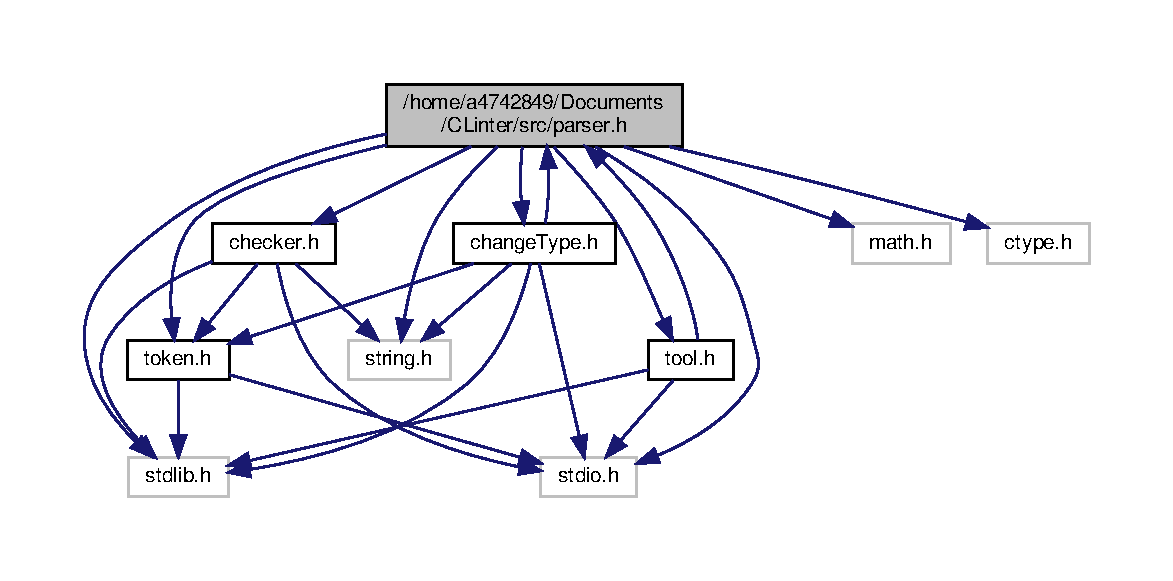
\includegraphics[width=350pt]{parser_8h__incl}
\end{center}
\end{figure}
This graph shows which files directly or indirectly include this file\+:
\nopagebreak
\begin{figure}[H]
\begin{center}
\leavevmode
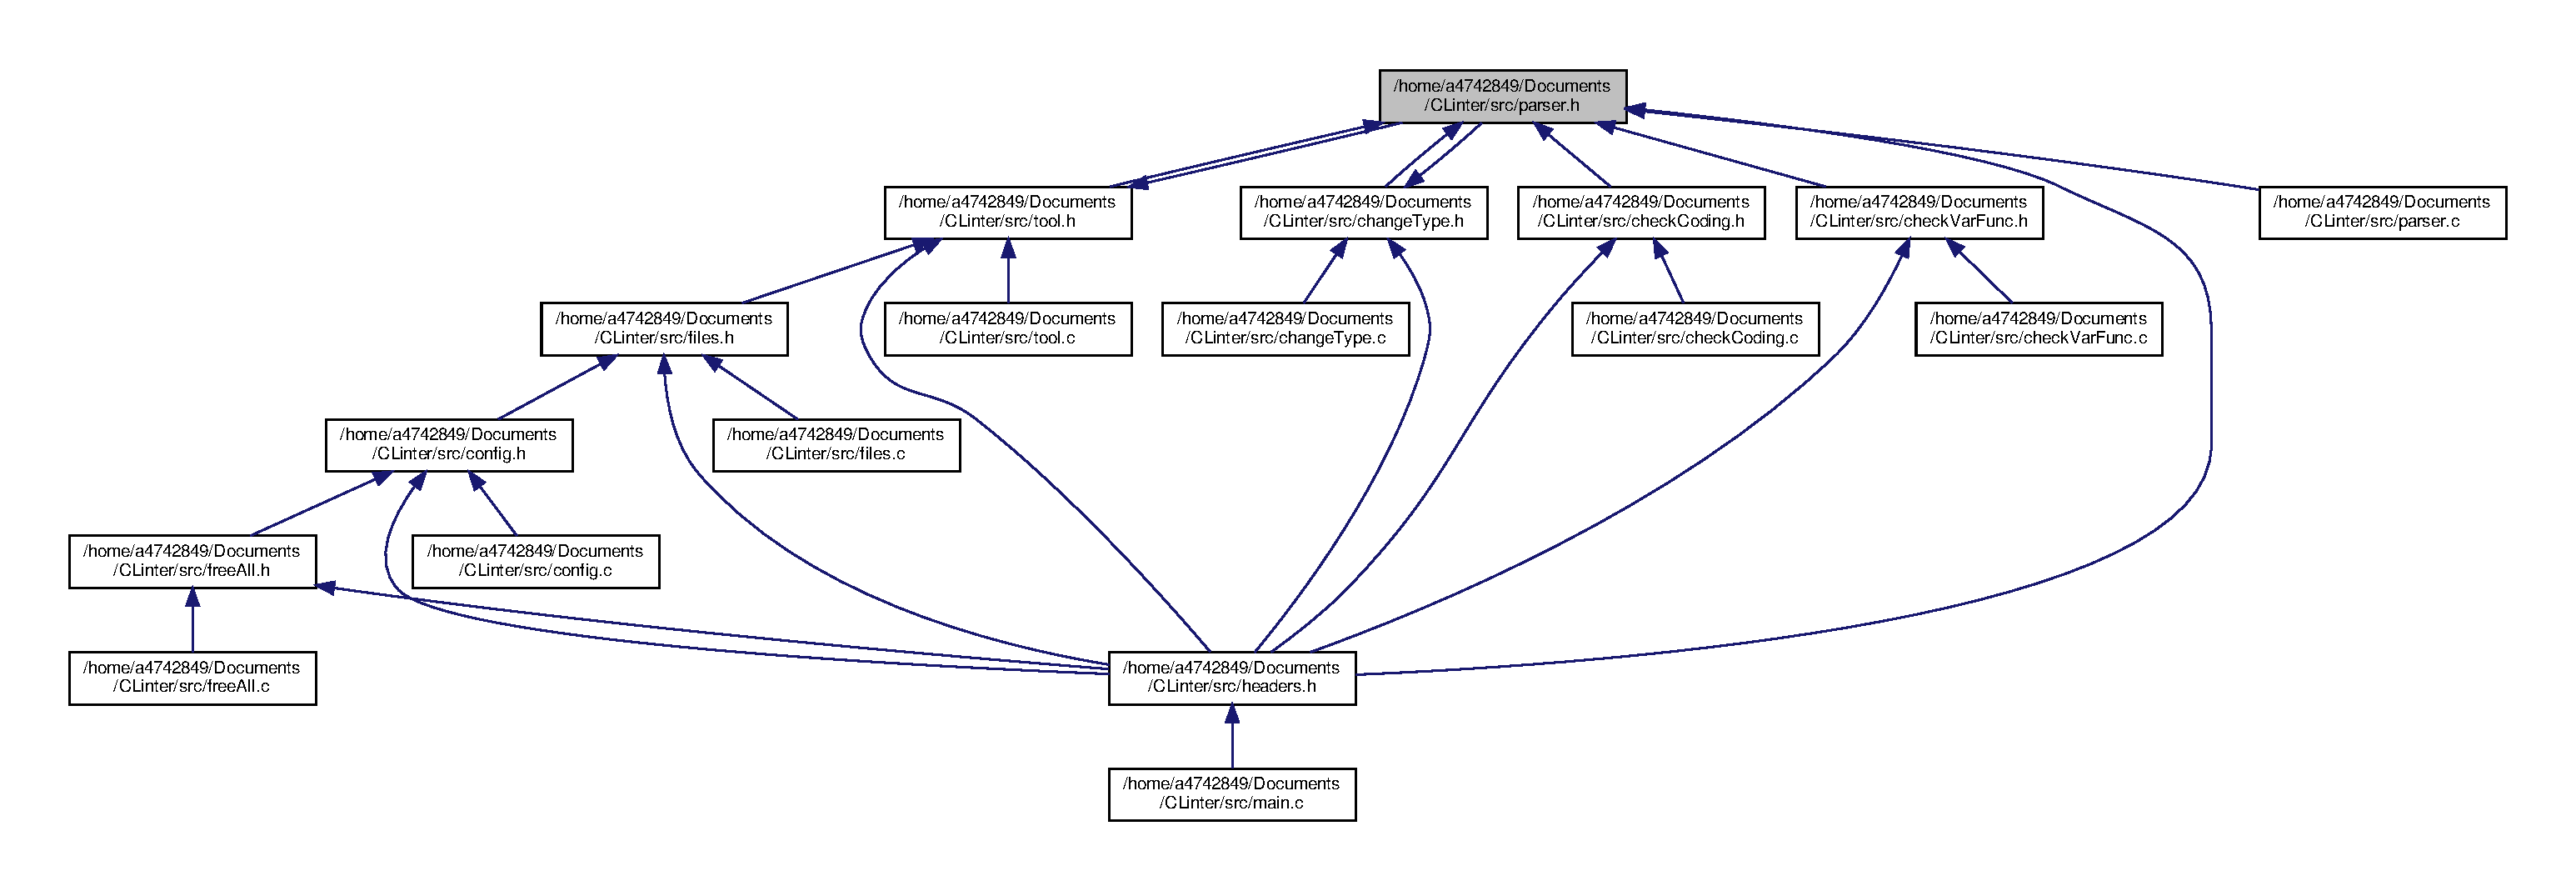
\includegraphics[width=350pt]{parser_8h__dep__incl}
\end{center}
\end{figure}
\subsection*{Macros}
\begin{DoxyCompactItemize}
\item 
\#define \hyperlink{parser_8h_a8d23feea868a983c8c2b661e1e16972f}{R\+ED}~\char`\"{}\textbackslash{}x1B\mbox{[}31m\char`\"{}
\begin{DoxyCompactList}\small\item\em Color Macro for pretty printing in R\+ED. \end{DoxyCompactList}\item 
\#define \hyperlink{parser_8h_a96fac03c4ab3363f06a0328e0e53a40c}{Y\+EL}~\char`\"{}\textbackslash{}x1B\mbox{[}33m\char`\"{}
\begin{DoxyCompactList}\small\item\em Color Macro for pretty printing in Y\+E\+L\+L\+OW. \end{DoxyCompactList}\item 
\#define \hyperlink{parser_8h_ab702106cf3b3e96750b6845ded4e0299}{R\+E\+S\+ET}~\char`\"{}\textbackslash{}x1B\mbox{[}0m\char`\"{}
\begin{DoxyCompactList}\small\item\em Reset to default color the printing color. \end{DoxyCompactList}\end{DoxyCompactItemize}
\subsection*{Functions}
\begin{DoxyCompactItemize}
\item 
\hyperlink{token_8h_af79b1a4f53ad41cc0de4b364b9455dba}{Token} $\ast$$\ast$ \hyperlink{parser_8h_adfdea08dc03111766b2a52dc0ffd9cb6}{parse} (char $\ast$str, int $\ast$nb\+Nodes)
\begin{DoxyCompactList}\small\item\em Reads a string and prints each token type. \end{DoxyCompactList}\item 
int \hyperlink{parser_8h_a32d638521fed670f56092d9220f17186}{is\+Ope} (char c)
\begin{DoxyCompactList}\small\item\em Tell if char is an operator. \end{DoxyCompactList}\item 
int \hyperlink{parser_8h_aa0c754508d5d35e6b7ca295174004323}{is\+Delim} (char c)
\begin{DoxyCompactList}\small\item\em Tell if char is a delimiter + operator. \end{DoxyCompactList}\item 
int \hyperlink{parser_8h_a5c8cb0c9a3afe1950d34267cfe898bc9}{is\+Delim\+No\+Space} (char c)
\begin{DoxyCompactList}\small\item\em Tell if char is a delimiter expect space \textquotesingle{} \textquotesingle{}. \end{DoxyCompactList}\item 
char $\ast$ \hyperlink{parser_8h_aa4859689aab814e043959441bf90f146}{get\+Sub\+String} (char $\ast$str, int left, int right)
\begin{DoxyCompactList}\small\item\em Get sub\+String of str delimited by left and right. \end{DoxyCompactList}\end{DoxyCompactItemize}


\subsection{Detailed Description}
This header file will contain all required definitions and basic utilities functions to transform text into Tokens. 

\begin{DoxyAuthor}{Author}
Antoine T\+A\+V\+E\+R\+N\+I\+ER
\end{DoxyAuthor}
\begin{DoxyDate}{Date}
16/11/2018 
\end{DoxyDate}


\subsection{Macro Definition Documentation}
\mbox{\Hypertarget{parser_8h_a8d23feea868a983c8c2b661e1e16972f}\label{parser_8h_a8d23feea868a983c8c2b661e1e16972f}} 
\index{parser.\+h@{parser.\+h}!R\+ED@{R\+ED}}
\index{R\+ED@{R\+ED}!parser.\+h@{parser.\+h}}
\subsubsection{\texorpdfstring{R\+ED}{RED}}
{\footnotesize\ttfamily \#define R\+ED~\char`\"{}\textbackslash{}x1B\mbox{[}31m\char`\"{}}



Color Macro for pretty printing in R\+ED. 

\mbox{\Hypertarget{parser_8h_ab702106cf3b3e96750b6845ded4e0299}\label{parser_8h_ab702106cf3b3e96750b6845ded4e0299}} 
\index{parser.\+h@{parser.\+h}!R\+E\+S\+ET@{R\+E\+S\+ET}}
\index{R\+E\+S\+ET@{R\+E\+S\+ET}!parser.\+h@{parser.\+h}}
\subsubsection{\texorpdfstring{R\+E\+S\+ET}{RESET}}
{\footnotesize\ttfamily \#define R\+E\+S\+ET~\char`\"{}\textbackslash{}x1B\mbox{[}0m\char`\"{}}



Reset to default color the printing color. 

\mbox{\Hypertarget{parser_8h_a96fac03c4ab3363f06a0328e0e53a40c}\label{parser_8h_a96fac03c4ab3363f06a0328e0e53a40c}} 
\index{parser.\+h@{parser.\+h}!Y\+EL@{Y\+EL}}
\index{Y\+EL@{Y\+EL}!parser.\+h@{parser.\+h}}
\subsubsection{\texorpdfstring{Y\+EL}{YEL}}
{\footnotesize\ttfamily \#define Y\+EL~\char`\"{}\textbackslash{}x1B\mbox{[}33m\char`\"{}}



Color Macro for pretty printing in Y\+E\+L\+L\+OW. 



\subsection{Function Documentation}
\mbox{\Hypertarget{parser_8h_aa4859689aab814e043959441bf90f146}\label{parser_8h_aa4859689aab814e043959441bf90f146}} 
\index{parser.\+h@{parser.\+h}!get\+Sub\+String@{get\+Sub\+String}}
\index{get\+Sub\+String@{get\+Sub\+String}!parser.\+h@{parser.\+h}}
\subsubsection{\texorpdfstring{get\+Sub\+String()}{getSubString()}}
{\footnotesize\ttfamily char$\ast$ get\+Sub\+String (\begin{DoxyParamCaption}\item[{char $\ast$}]{str,  }\item[{int}]{left,  }\item[{int}]{right }\end{DoxyParamCaption})}



Get sub\+String of str delimited by left and right. 


\begin{DoxyParams}{Parameters}
{\em str} & String containing text \\
\hline
{\em left} & Left pointer on the str \\
\hline
{\em right} & Right pointer on the str \\
\hline
\end{DoxyParams}
\begin{DoxyReturn}{Returns}
char$\ast$ Substring between left and right pointers 
\end{DoxyReturn}
\mbox{\Hypertarget{parser_8h_aa0c754508d5d35e6b7ca295174004323}\label{parser_8h_aa0c754508d5d35e6b7ca295174004323}} 
\index{parser.\+h@{parser.\+h}!is\+Delim@{is\+Delim}}
\index{is\+Delim@{is\+Delim}!parser.\+h@{parser.\+h}}
\subsubsection{\texorpdfstring{is\+Delim()}{isDelim()}}
{\footnotesize\ttfamily int is\+Delim (\begin{DoxyParamCaption}\item[{char}]{c }\end{DoxyParamCaption})}



Tell if char is a delimiter + operator. 


\begin{DoxyParams}{Parameters}
{\em c} & character to check \\
\hline
\end{DoxyParams}
\begin{DoxyReturn}{Returns}
int 0 false else true 
\end{DoxyReturn}
\mbox{\Hypertarget{parser_8h_a5c8cb0c9a3afe1950d34267cfe898bc9}\label{parser_8h_a5c8cb0c9a3afe1950d34267cfe898bc9}} 
\index{parser.\+h@{parser.\+h}!is\+Delim\+No\+Space@{is\+Delim\+No\+Space}}
\index{is\+Delim\+No\+Space@{is\+Delim\+No\+Space}!parser.\+h@{parser.\+h}}
\subsubsection{\texorpdfstring{is\+Delim\+No\+Space()}{isDelimNoSpace()}}
{\footnotesize\ttfamily int is\+Delim\+No\+Space (\begin{DoxyParamCaption}\item[{char}]{c }\end{DoxyParamCaption})}



Tell if char is a delimiter expect space \textquotesingle{} \textquotesingle{}. 


\begin{DoxyParams}{Parameters}
{\em c} & character to check \\
\hline
\end{DoxyParams}
\begin{DoxyReturn}{Returns}
int 0 false else true 
\end{DoxyReturn}
\mbox{\Hypertarget{parser_8h_a32d638521fed670f56092d9220f17186}\label{parser_8h_a32d638521fed670f56092d9220f17186}} 
\index{parser.\+h@{parser.\+h}!is\+Ope@{is\+Ope}}
\index{is\+Ope@{is\+Ope}!parser.\+h@{parser.\+h}}
\subsubsection{\texorpdfstring{is\+Ope()}{isOpe()}}
{\footnotesize\ttfamily int is\+Ope (\begin{DoxyParamCaption}\item[{char}]{c }\end{DoxyParamCaption})}



Tell if char is an operator. 


\begin{DoxyParams}{Parameters}
{\em c} & character to check \\
\hline
\end{DoxyParams}
\begin{DoxyReturn}{Returns}
int 0 false else true 
\end{DoxyReturn}
\mbox{\Hypertarget{parser_8h_adfdea08dc03111766b2a52dc0ffd9cb6}\label{parser_8h_adfdea08dc03111766b2a52dc0ffd9cb6}} 
\index{parser.\+h@{parser.\+h}!parse@{parse}}
\index{parse@{parse}!parser.\+h@{parser.\+h}}
\subsubsection{\texorpdfstring{parse()}{parse()}}
{\footnotesize\ttfamily \hyperlink{token_8h_af79b1a4f53ad41cc0de4b364b9455dba}{Token}$\ast$$\ast$ parse (\begin{DoxyParamCaption}\item[{char $\ast$}]{str,  }\item[{int $\ast$}]{nb\+Nodes }\end{DoxyParamCaption})}



Reads a string and prints each token type. 


\begin{DoxyParams}{Parameters}
{\em str} & input string (code from given file) \\
\hline
{\em nb\+Nodes} & number of nodes in string \\
\hline
\end{DoxyParams}
\begin{DoxyReturn}{Returns}
Token$\ast$$\ast$ list of list of tokens 
\end{DoxyReturn}

\hypertarget{token_8c}{}\section{/home/a4742849/\+Documents/\+C\+Linter/src/token.c File Reference}
\label{token_8c}\index{/home/a4742849/\+Documents/\+C\+Linter/src/token.\+c@{/home/a4742849/\+Documents/\+C\+Linter/src/token.\+c}}


This c file will contain all functions to create a Token.  


{\ttfamily \#include \char`\"{}token.\+h\char`\"{}}\newline
Include dependency graph for token.\+c\+:\nopagebreak
\begin{figure}[H]
\begin{center}
\leavevmode
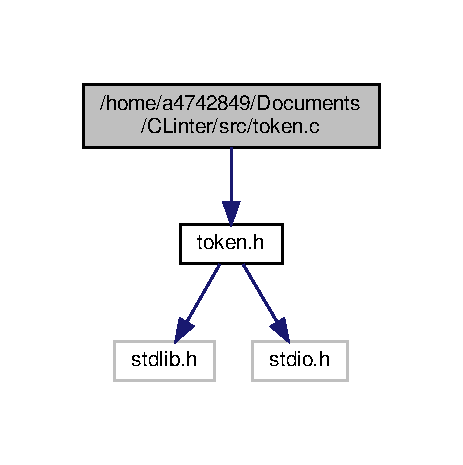
\includegraphics[width=222pt]{token_8c__incl}
\end{center}
\end{figure}
\subsection*{Functions}
\begin{DoxyCompactItemize}
\item 
char $\ast$ \hyperlink{token_8c_ac0b85853d622a09357cdda081995170c}{get\+Enum\+Name} (\hyperlink{token_8h_a16a6868f96564b3446a7f86b122b253e}{Type} type)
\begin{DoxyCompactList}\small\item\em Get the Enum Name of a Type. \end{DoxyCompactList}\item 
\hyperlink{token_8h_af79b1a4f53ad41cc0de4b364b9455dba}{Token} $\ast$ \hyperlink{token_8c_abebe689541881c2fe2c2ea2b516dd2c0}{create\+Token} (\hyperlink{token_8h_a16a6868f96564b3446a7f86b122b253e}{Type} type, char $\ast$value, int pos)
\begin{DoxyCompactList}\small\item\em Create a Token structure. \end{DoxyCompactList}\end{DoxyCompactItemize}


\subsection{Detailed Description}
This c file will contain all functions to create a Token. 

\begin{DoxyAuthor}{Author}
Antoine T\+A\+V\+E\+R\+N\+I\+ER
\end{DoxyAuthor}
\begin{DoxyDate}{Date}
16/11/2018 
\end{DoxyDate}


\subsection{Function Documentation}
\mbox{\Hypertarget{token_8c_abebe689541881c2fe2c2ea2b516dd2c0}\label{token_8c_abebe689541881c2fe2c2ea2b516dd2c0}} 
\index{token.\+c@{token.\+c}!create\+Token@{create\+Token}}
\index{create\+Token@{create\+Token}!token.\+c@{token.\+c}}
\subsubsection{\texorpdfstring{create\+Token()}{createToken()}}
{\footnotesize\ttfamily \hyperlink{token_8h_af79b1a4f53ad41cc0de4b364b9455dba}{Token}$\ast$ create\+Token (\begin{DoxyParamCaption}\item[{\hyperlink{token_8h_a16a6868f96564b3446a7f86b122b253e}{Type}}]{type,  }\item[{char $\ast$}]{value,  }\item[{int}]{pos }\end{DoxyParamCaption})}



Create a Token structure. 


\begin{DoxyParams}{Parameters}
{\em type} & Given Type \\
\hline
{\em value} & Given String value \\
\hline
{\em pos} & Given position of the Token in a line \\
\hline
\end{DoxyParams}
\begin{DoxyReturn}{Returns}
Token$\ast$ A new Token 
\end{DoxyReturn}
\mbox{\Hypertarget{token_8c_ac0b85853d622a09357cdda081995170c}\label{token_8c_ac0b85853d622a09357cdda081995170c}} 
\index{token.\+c@{token.\+c}!get\+Enum\+Name@{get\+Enum\+Name}}
\index{get\+Enum\+Name@{get\+Enum\+Name}!token.\+c@{token.\+c}}
\subsubsection{\texorpdfstring{get\+Enum\+Name()}{getEnumName()}}
{\footnotesize\ttfamily char$\ast$ get\+Enum\+Name (\begin{DoxyParamCaption}\item[{\hyperlink{token_8h_a16a6868f96564b3446a7f86b122b253e}{Type}}]{type }\end{DoxyParamCaption})}



Get the Enum Name of a Type. 


\begin{DoxyParams}{Parameters}
{\em type} & Given Type \\
\hline
\end{DoxyParams}
\begin{DoxyReturn}{Returns}
char$\ast$ Type cast to string 
\end{DoxyReturn}

\hypertarget{token_8h}{}\section{/home/a4742849/\+Documents/\+C\+Linter/src/token.h File Reference}
\label{token_8h}\index{/home/a4742849/\+Documents/\+C\+Linter/src/token.\+h@{/home/a4742849/\+Documents/\+C\+Linter/src/token.\+h}}


This header file will contain all required definitions and basic utilities functions to create a Token.  


{\ttfamily \#include $<$stdlib.\+h$>$}\newline
{\ttfamily \#include $<$stdio.\+h$>$}\newline
Include dependency graph for token.\+h\+:\nopagebreak
\begin{figure}[H]
\begin{center}
\leavevmode
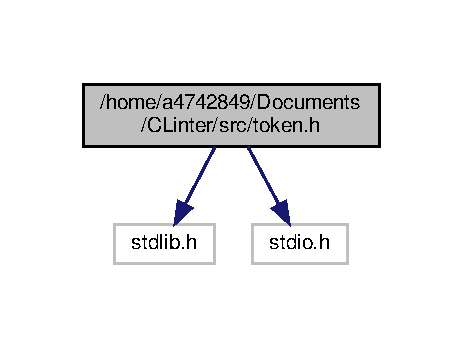
\includegraphics[width=222pt]{token_8h__incl}
\end{center}
\end{figure}
This graph shows which files directly or indirectly include this file\+:
\nopagebreak
\begin{figure}[H]
\begin{center}
\leavevmode
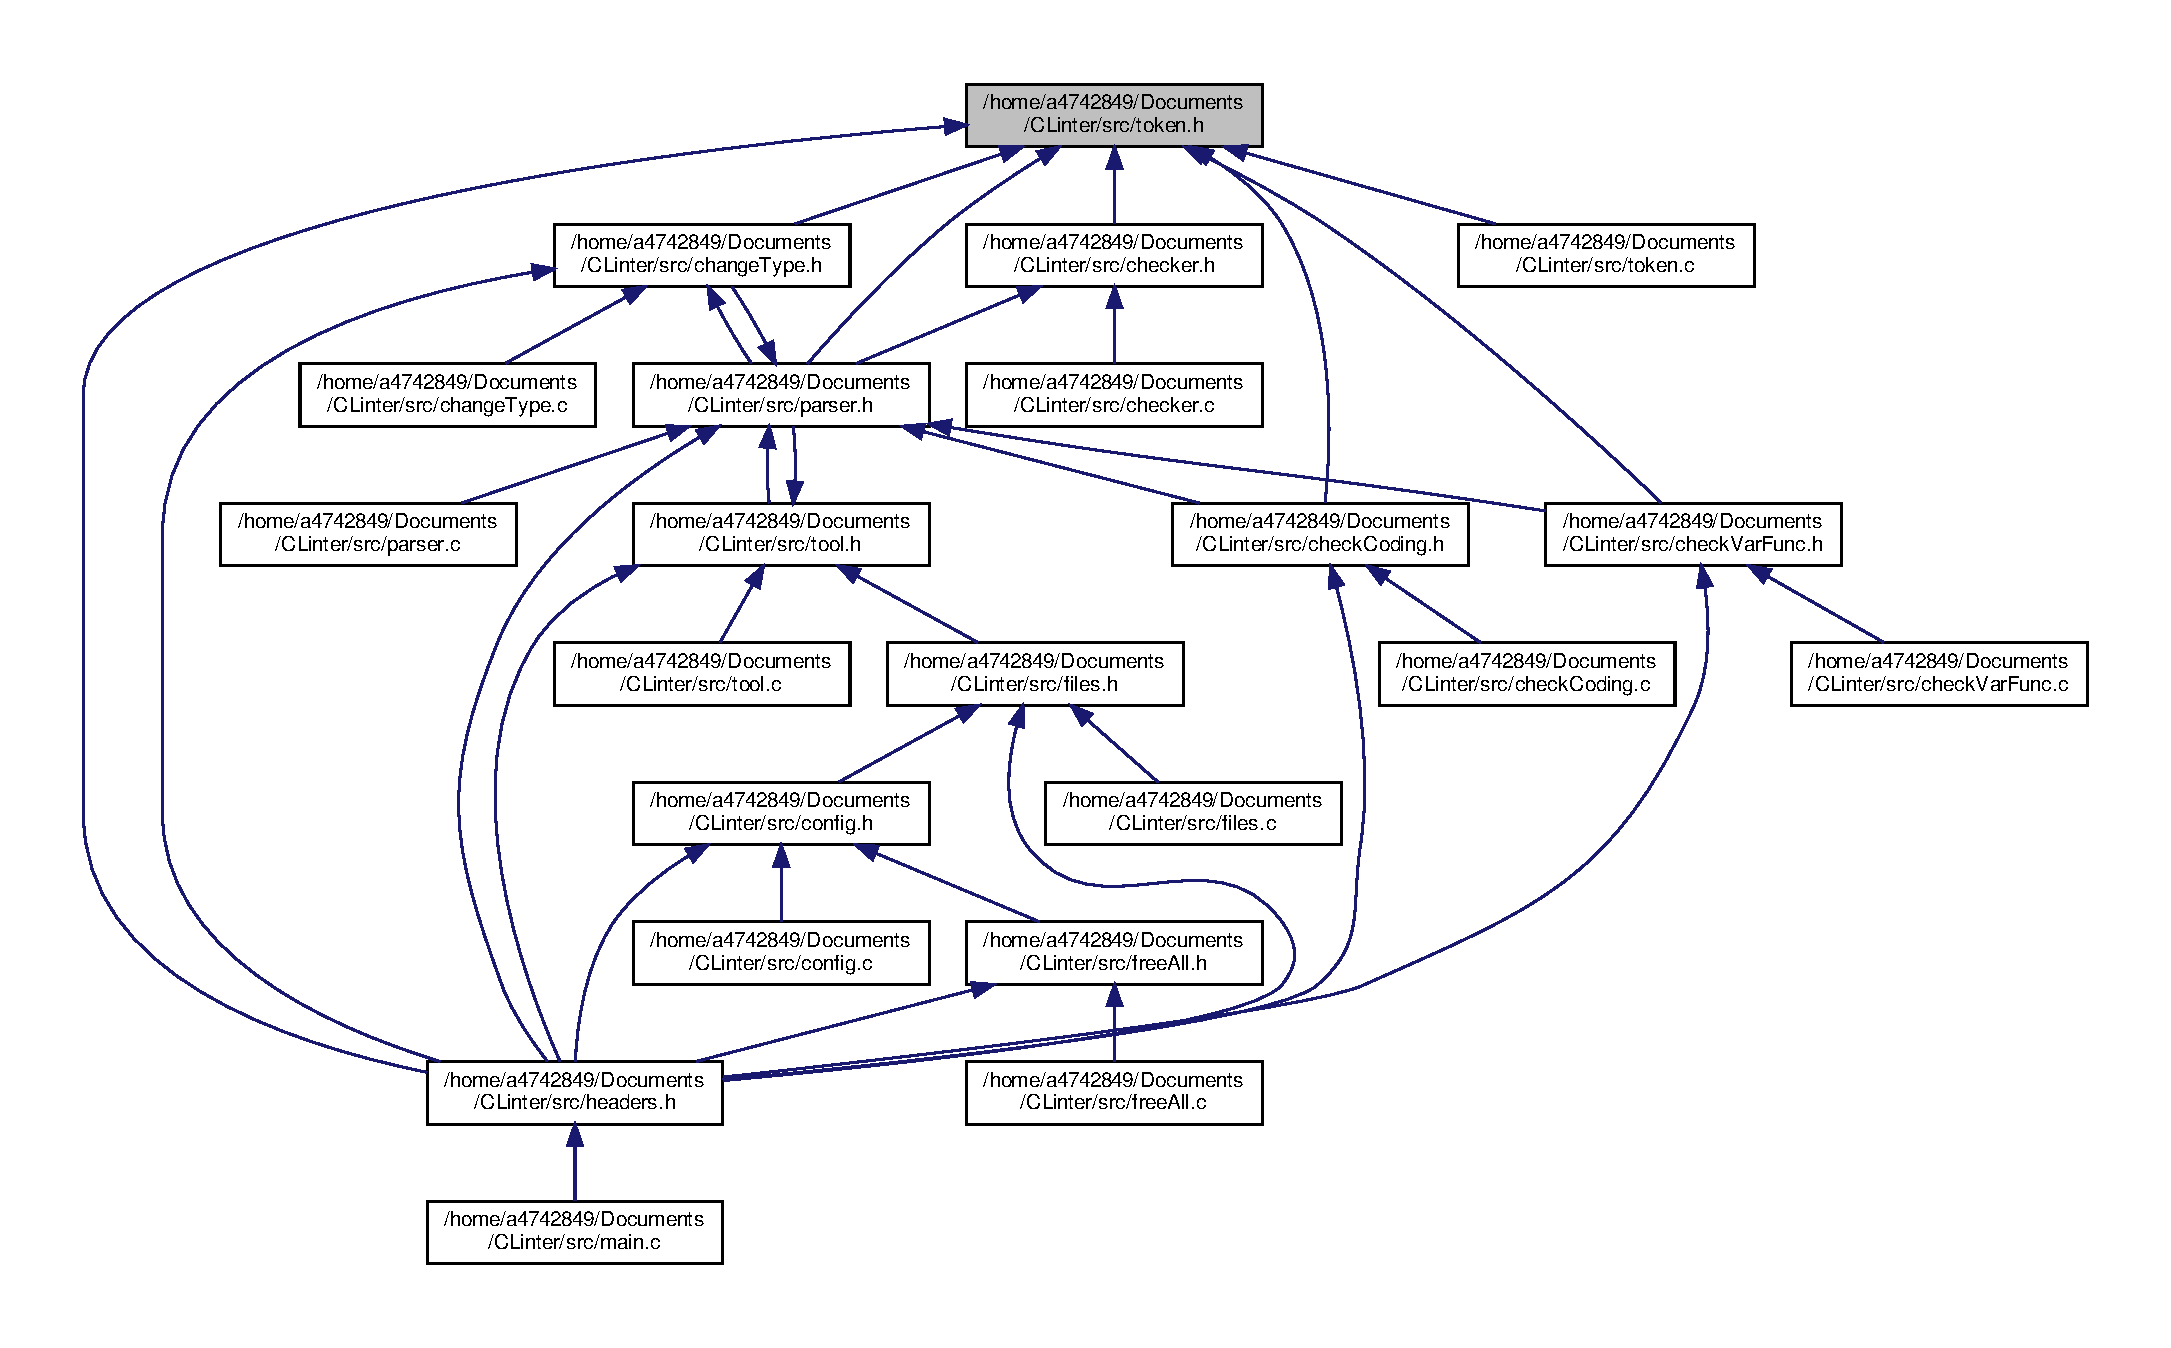
\includegraphics[width=350pt]{token_8h__dep__incl}
\end{center}
\end{figure}
\subsection*{Classes}
\begin{DoxyCompactItemize}
\item 
struct \hyperlink{structToken__t}{Token\+\_\+t}
\begin{DoxyCompactList}\small\item\em Structure to store a Token. \end{DoxyCompactList}\end{DoxyCompactItemize}
\subsection*{Typedefs}
\begin{DoxyCompactItemize}
\item 
typedef enum \hyperlink{token_8h_a52fe9583fb1d702f7e0e065420c15f0b}{Type\+\_\+e} \hyperlink{token_8h_a16a6868f96564b3446a7f86b122b253e}{Type}
\begin{DoxyCompactList}\small\item\em Enumeration to store type of a Token. \end{DoxyCompactList}\item 
typedef struct \hyperlink{structToken__t}{Token\+\_\+t} \hyperlink{token_8h_af79b1a4f53ad41cc0de4b364b9455dba}{Token}
\begin{DoxyCompactList}\small\item\em Structure to store a Token. \end{DoxyCompactList}\end{DoxyCompactItemize}
\subsection*{Enumerations}
\begin{DoxyCompactItemize}
\item 
enum \hyperlink{token_8h_a52fe9583fb1d702f7e0e065420c15f0b}{Type\+\_\+e} \{ \newline
\hyperlink{token_8h_a52fe9583fb1d702f7e0e065420c15f0bac6ea0269d59d3016f1f6a3f4240b71f8}{Operator}, 
\hyperlink{token_8h_a52fe9583fb1d702f7e0e065420c15f0ba3c492934fcc5b03d26f735174385bbfc}{Delimiter}, 
\hyperlink{token_8h_a52fe9583fb1d702f7e0e065420c15f0ba18c03e9114911894d062ca85749aeed9}{Variable}, 
\hyperlink{token_8h_a52fe9583fb1d702f7e0e065420c15f0baf2b400cf2347c8b1886e2bd386c5b59d}{Numerical}, 
\newline
\hyperlink{token_8h_a52fe9583fb1d702f7e0e065420c15f0bacc1bf97b199ded936412816f47c79de2}{Key\+Word}, 
\hyperlink{token_8h_a52fe9583fb1d702f7e0e065420c15f0baf06db7f5f71e7d3ba1c68fa7ee7f08ca}{Var\+\_\+type}, 
\hyperlink{token_8h_a52fe9583fb1d702f7e0e065420c15f0ba7eec5006696b611a5cd6514537a57c62}{Open\+Par}, 
\hyperlink{token_8h_a52fe9583fb1d702f7e0e065420c15f0bafc7f4e12253ee22fa9c7b8ce97b1561f}{Closed\+Par}, 
\newline
\hyperlink{token_8h_a52fe9583fb1d702f7e0e065420c15f0babd0b898766621e7a90704b6716be798e}{Open\+Bracket}, 
\hyperlink{token_8h_a52fe9583fb1d702f7e0e065420c15f0ba45a8944e2ef057c2fb1ecfa93dc9b73c}{Closed\+Bracket}, 
\hyperlink{token_8h_a52fe9583fb1d702f7e0e065420c15f0ba7a78e5b3c82a0150e5f90f5d994d1584}{Dot\+Coma}, 
\hyperlink{token_8h_a52fe9583fb1d702f7e0e065420c15f0bace00e32f2eab15c41614a4ca4d50d794}{C\+O\+MA}, 
\newline
\hyperlink{token_8h_a52fe9583fb1d702f7e0e065420c15f0ba84f8ae2490f9e4bd2321fd21f4b0e807}{I\+D\+E\+N\+T\+I\+F\+I\+ER}, 
\hyperlink{token_8h_a52fe9583fb1d702f7e0e065420c15f0ba83972670b57415508523b5641bb46116}{C\+O\+N\+S\+T\+A\+NT}, 
\hyperlink{token_8h_a52fe9583fb1d702f7e0e065420c15f0ba655e632575aa38fd0f04138439932a22}{S\+T\+R\+I\+N\+G\+\_\+\+L\+I\+T\+E\+R\+AL}, 
\hyperlink{token_8h_a52fe9583fb1d702f7e0e065420c15f0ba0d62820bd83927b91b7ddf71280b6e24}{P\+T\+R\+\_\+\+OP}, 
\newline
\hyperlink{token_8h_a52fe9583fb1d702f7e0e065420c15f0bac50cdb81935e91bed6840c116a10401b}{I\+N\+C\+\_\+\+OP}, 
\hyperlink{token_8h_a52fe9583fb1d702f7e0e065420c15f0ba926f5c40b46a49423f1fb0224614e9e5}{D\+E\+C\+\_\+\+OP}, 
\hyperlink{token_8h_a52fe9583fb1d702f7e0e065420c15f0baacf3a9a27bdfb0bd9fba6a5420768f06}{S\+I\+Z\+E\+OF}, 
\hyperlink{token_8h_a52fe9583fb1d702f7e0e065420c15f0bae54b9c7f6630f8d947c3ce9b23c735ab}{L\+E\+F\+T\+\_\+\+OP}, 
\newline
\hyperlink{token_8h_a52fe9583fb1d702f7e0e065420c15f0ba472e10f0b9c73771cfeea06df95f8393}{R\+I\+G\+H\+T\+\_\+\+OP}, 
\hyperlink{token_8h_a52fe9583fb1d702f7e0e065420c15f0bac651601a6d9cb11e92a2f131415cbeaf}{L\+E\+\_\+\+OP}, 
\hyperlink{token_8h_a52fe9583fb1d702f7e0e065420c15f0ba3cf773750faa5bfc6f64f0dd92ab85b6}{G\+E\+\_\+\+OP}, 
\hyperlink{token_8h_a52fe9583fb1d702f7e0e065420c15f0ba3f66f225e0b0a87c7be82b63f6cdb5c7}{E\+Q\+\_\+\+OP}, 
\newline
\hyperlink{token_8h_a52fe9583fb1d702f7e0e065420c15f0ba3b08c224b7bf164b1fb28b7b37c2071b}{N\+E\+\_\+\+OP}, 
\hyperlink{token_8h_a52fe9583fb1d702f7e0e065420c15f0ba634867e3dac3e0ae6098caf0cd873a61}{A\+N\+D\+\_\+\+OP}, 
\hyperlink{token_8h_a52fe9583fb1d702f7e0e065420c15f0ba15d48b8e2dfd351bfbd4b8338275fe05}{O\+R\+\_\+\+OP}, 
\hyperlink{token_8h_a52fe9583fb1d702f7e0e065420c15f0bab3b523dbe5c7cfa6e419e1b5e67756dd}{M\+U\+L\+\_\+\+A\+S\+S\+I\+GN}, 
\newline
\hyperlink{token_8h_a52fe9583fb1d702f7e0e065420c15f0baf35daa301b6d7db00f1f99626284f7a9}{D\+I\+V\+\_\+\+A\+S\+S\+I\+GN}, 
\hyperlink{token_8h_a52fe9583fb1d702f7e0e065420c15f0ba8dab714ebb18a208c08cce15323a660f}{M\+O\+D\+\_\+\+A\+S\+S\+I\+GN}, 
\hyperlink{token_8h_a52fe9583fb1d702f7e0e065420c15f0ba4ce372cd3237d2180971ac1779ab4199}{A\+D\+D\+\_\+\+A\+S\+S\+I\+GN}, 
\hyperlink{token_8h_a52fe9583fb1d702f7e0e065420c15f0baa1c03d53b204212d180e44ac93c63ece}{S\+U\+B\+\_\+\+A\+S\+S\+I\+GN}, 
\newline
\hyperlink{token_8h_a52fe9583fb1d702f7e0e065420c15f0babbad2dbb961a10d3c05be06dec1e64a8}{L\+E\+F\+T\+\_\+\+A\+S\+S\+I\+GN}, 
\hyperlink{token_8h_a52fe9583fb1d702f7e0e065420c15f0ba84e44e673145bddc3e6dbb324bfffd7f}{R\+I\+G\+H\+T\+\_\+\+A\+S\+S\+I\+GN}, 
\hyperlink{token_8h_a52fe9583fb1d702f7e0e065420c15f0ba4d17533bee0fb5c6bd8209adeb1ca40a}{A\+N\+D\+\_\+\+A\+S\+S\+I\+GN}, 
\hyperlink{token_8h_a52fe9583fb1d702f7e0e065420c15f0bacd83325057c9334202665de437146575}{X\+O\+R\+\_\+\+A\+S\+S\+I\+GN}, 
\newline
\hyperlink{token_8h_a52fe9583fb1d702f7e0e065420c15f0ba83006db00b27c9c6866c1767725fd751}{O\+R\+\_\+\+A\+S\+S\+I\+GN}, 
\hyperlink{token_8h_a52fe9583fb1d702f7e0e065420c15f0ba802d02227696a7c5b5420b28d8b82338}{T\+Y\+P\+E\+D\+EF}, 
\hyperlink{token_8h_a52fe9583fb1d702f7e0e065420c15f0baf017da8df4e93d9bc75880a4998c1039}{E\+X\+T\+E\+RN}, 
\hyperlink{token_8h_a52fe9583fb1d702f7e0e065420c15f0bae55a36a850c67d46b3b3325de7fce0b8}{S\+T\+A\+T\+IC}, 
\newline
\hyperlink{token_8h_a52fe9583fb1d702f7e0e065420c15f0baeef9468d1b98bca652a04bf5063fd9d6}{A\+U\+TO}, 
\hyperlink{token_8h_a52fe9583fb1d702f7e0e065420c15f0baceb7c305772dab23a260960771180df3}{R\+E\+G\+I\+S\+T\+ER}, 
\hyperlink{token_8h_a52fe9583fb1d702f7e0e065420c15f0badb31f5ef7acca5e1131fcc0fbfa6911d}{V\+O\+ID}, 
\hyperlink{token_8h_a52fe9583fb1d702f7e0e065420c15f0ba4618cf21306b3c647741afa7ebefcab8}{C\+H\+AR}, 
\newline
\hyperlink{token_8h_a52fe9583fb1d702f7e0e065420c15f0ba7a1fe3ba88f0c16cb494922948a9597d}{S\+H\+O\+RT}, 
\hyperlink{token_8h_a52fe9583fb1d702f7e0e065420c15f0bafd5a5f51ce25953f3db2c7e93eb7864a}{I\+NT}, 
\hyperlink{token_8h_a52fe9583fb1d702f7e0e065420c15f0baaee055c4a5aba7d55774e4f1c01dacea}{L\+O\+NG}, 
\hyperlink{token_8h_a52fe9583fb1d702f7e0e065420c15f0ba9cf4a0866224b0bb4a7a895da27c9c4c}{F\+L\+O\+AT}, 
\newline
\hyperlink{token_8h_a52fe9583fb1d702f7e0e065420c15f0ba33465d1d419b1074fb259ef444609e92}{D\+O\+U\+B\+LE}, 
\hyperlink{token_8h_a52fe9583fb1d702f7e0e065420c15f0ba7efc726d1072390f5ff31166cc4c1b6f}{S\+I\+G\+N\+ED}, 
\hyperlink{token_8h_a52fe9583fb1d702f7e0e065420c15f0ba7165f9a47792f47c718ca128556fb3ae}{U\+N\+S\+I\+G\+N\+ED}, 
\hyperlink{token_8h_a52fe9583fb1d702f7e0e065420c15f0baa6846b35058c4f14c56b52b60cdbed67}{T\+Y\+P\+E\+\_\+\+N\+A\+ME}, 
\newline
\hyperlink{token_8h_a52fe9583fb1d702f7e0e065420c15f0ba840fc36796c5af05b4616165e6449dad}{S\+T\+R\+U\+CT}, 
\hyperlink{token_8h_a52fe9583fb1d702f7e0e065420c15f0ba4cf5e96eb7880eb38df303a6e5759afd}{U\+N\+I\+ON}, 
\hyperlink{token_8h_a52fe9583fb1d702f7e0e065420c15f0ba5bc38f5ef3a09fbc02c3f3576277a5b9}{E\+N\+UM}, 
\hyperlink{token_8h_a52fe9583fb1d702f7e0e065420c15f0ba3d044162d972156d897cea80f216b9ca}{C\+O\+N\+ST}, 
\newline
\hyperlink{token_8h_a52fe9583fb1d702f7e0e065420c15f0bad2cbe40cd1e913a07a0d702786a14922}{V\+O\+L\+A\+T\+I\+LE}, 
\hyperlink{token_8h_a52fe9583fb1d702f7e0e065420c15f0ba18b0e195bead02564c90768cc4942cca}{E\+L\+L\+I\+P\+S\+IS}, 
\hyperlink{token_8h_a52fe9583fb1d702f7e0e065420c15f0ba9c9b14644e9370719a51b7342bbc9c4d}{C\+A\+SE}, 
\hyperlink{token_8h_a52fe9583fb1d702f7e0e065420c15f0ba88ec7d5086d2469ba843c7fcceade8a6}{D\+E\+F\+A\+U\+LT}, 
\newline
\hyperlink{token_8h_a52fe9583fb1d702f7e0e065420c15f0ba252802eda493fb6b4a279c4452acb547}{IF}, 
\hyperlink{token_8h_a52fe9583fb1d702f7e0e065420c15f0ba90d649d830ea440c8b8a56c7ef23c426}{E\+L\+SE}, 
\hyperlink{token_8h_a52fe9583fb1d702f7e0e065420c15f0ba53396ea1193548270407675ea4eeee2b}{S\+W\+I\+T\+CH}, 
\hyperlink{token_8h_a52fe9583fb1d702f7e0e065420c15f0ba3278fd035226215822c903790a1eee73}{W\+H\+I\+LE}, 
\newline
\hyperlink{token_8h_a52fe9583fb1d702f7e0e065420c15f0babfea6036e64d9c7c773d277a57d2f959}{DO}, 
\hyperlink{token_8h_a52fe9583fb1d702f7e0e065420c15f0baa809654855caa62449850d9122fd77a8}{F\+OR}, 
\hyperlink{token_8h_a52fe9583fb1d702f7e0e065420c15f0badf1256e4198172eedfbf12c770d11589}{G\+O\+TO}, 
\hyperlink{token_8h_a52fe9583fb1d702f7e0e065420c15f0ba49959dd441dcda75d6898cf2c68fb374}{C\+O\+N\+T\+I\+N\+UE}, 
\newline
\hyperlink{token_8h_a52fe9583fb1d702f7e0e065420c15f0ba9524d094809858b9e4f778763913568a}{B\+R\+E\+AK}, 
\hyperlink{token_8h_a52fe9583fb1d702f7e0e065420c15f0ba520e09ffec033636dba711f3441cc600}{R\+E\+T\+U\+RN}, 
\hyperlink{token_8h_a52fe9583fb1d702f7e0e065420c15f0bac08dae7edcb5c5bb959fee5971fbad95}{S\+P\+A\+CE}, 
\hyperlink{token_8h_a52fe9583fb1d702f7e0e065420c15f0ba920380215591395ea33ee5df8e293e19}{T\+AB}, 
\newline
\hyperlink{token_8h_a52fe9583fb1d702f7e0e065420c15f0ba0b44d4e916221e52c4ba47a8efb5e2fc}{Nothing}
 \}\begin{DoxyCompactList}\small\item\em Enumeration to store type of a Token. \end{DoxyCompactList}
\end{DoxyCompactItemize}
\subsection*{Functions}
\begin{DoxyCompactItemize}
\item 
char $\ast$ \hyperlink{token_8h_ac0b85853d622a09357cdda081995170c}{get\+Enum\+Name} (\hyperlink{token_8h_a16a6868f96564b3446a7f86b122b253e}{Type} type)
\begin{DoxyCompactList}\small\item\em Get the Enum Name of a Type. \end{DoxyCompactList}\item 
\hyperlink{token_8h_af79b1a4f53ad41cc0de4b364b9455dba}{Token} $\ast$ \hyperlink{token_8h_abebe689541881c2fe2c2ea2b516dd2c0}{create\+Token} (\hyperlink{token_8h_a16a6868f96564b3446a7f86b122b253e}{Type} type, char $\ast$value, int pos)
\begin{DoxyCompactList}\small\item\em Create a Token structure. \end{DoxyCompactList}\end{DoxyCompactItemize}


\subsection{Detailed Description}
This header file will contain all required definitions and basic utilities functions to create a Token. 

\begin{DoxyAuthor}{Author}
Antoine T\+A\+V\+E\+R\+N\+I\+ER
\end{DoxyAuthor}
\begin{DoxyDate}{Date}
16/11/2018 
\end{DoxyDate}


\subsection{Typedef Documentation}
\mbox{\Hypertarget{token_8h_af79b1a4f53ad41cc0de4b364b9455dba}\label{token_8h_af79b1a4f53ad41cc0de4b364b9455dba}} 
\index{token.\+h@{token.\+h}!Token@{Token}}
\index{Token@{Token}!token.\+h@{token.\+h}}
\subsubsection{\texorpdfstring{Token}{Token}}
{\footnotesize\ttfamily typedef struct \hyperlink{structToken__t}{Token\+\_\+t}  \hyperlink{token_8h_af79b1a4f53ad41cc0de4b364b9455dba}{Token}}



Structure to store a Token. 

\mbox{\Hypertarget{token_8h_a16a6868f96564b3446a7f86b122b253e}\label{token_8h_a16a6868f96564b3446a7f86b122b253e}} 
\index{token.\+h@{token.\+h}!Type@{Type}}
\index{Type@{Type}!token.\+h@{token.\+h}}
\subsubsection{\texorpdfstring{Type}{Type}}
{\footnotesize\ttfamily typedef enum \hyperlink{token_8h_a52fe9583fb1d702f7e0e065420c15f0b}{Type\+\_\+e}  \hyperlink{token_8h_a16a6868f96564b3446a7f86b122b253e}{Type}}



Enumeration to store type of a Token. 



\subsection{Enumeration Type Documentation}
\mbox{\Hypertarget{token_8h_a52fe9583fb1d702f7e0e065420c15f0b}\label{token_8h_a52fe9583fb1d702f7e0e065420c15f0b}} 
\index{token.\+h@{token.\+h}!Type\+\_\+e@{Type\+\_\+e}}
\index{Type\+\_\+e@{Type\+\_\+e}!token.\+h@{token.\+h}}
\subsubsection{\texorpdfstring{Type\+\_\+e}{Type\_e}}
{\footnotesize\ttfamily enum \hyperlink{token_8h_a52fe9583fb1d702f7e0e065420c15f0b}{Type\+\_\+e}}



Enumeration to store type of a Token. 

\begin{DoxyEnumFields}{Enumerator}
\raisebox{\heightof{T}}[0pt][0pt]{\index{Operator@{Operator}!token.\+h@{token.\+h}}\index{token.\+h@{token.\+h}!Operator@{Operator}}}\mbox{\Hypertarget{token_8h_a52fe9583fb1d702f7e0e065420c15f0bac6ea0269d59d3016f1f6a3f4240b71f8}\label{token_8h_a52fe9583fb1d702f7e0e065420c15f0bac6ea0269d59d3016f1f6a3f4240b71f8}} 
Operator&\\
\hline

\raisebox{\heightof{T}}[0pt][0pt]{\index{Delimiter@{Delimiter}!token.\+h@{token.\+h}}\index{token.\+h@{token.\+h}!Delimiter@{Delimiter}}}\mbox{\Hypertarget{token_8h_a52fe9583fb1d702f7e0e065420c15f0ba3c492934fcc5b03d26f735174385bbfc}\label{token_8h_a52fe9583fb1d702f7e0e065420c15f0ba3c492934fcc5b03d26f735174385bbfc}} 
Delimiter&\\
\hline

\raisebox{\heightof{T}}[0pt][0pt]{\index{Variable@{Variable}!token.\+h@{token.\+h}}\index{token.\+h@{token.\+h}!Variable@{Variable}}}\mbox{\Hypertarget{token_8h_a52fe9583fb1d702f7e0e065420c15f0ba18c03e9114911894d062ca85749aeed9}\label{token_8h_a52fe9583fb1d702f7e0e065420c15f0ba18c03e9114911894d062ca85749aeed9}} 
Variable&\\
\hline

\raisebox{\heightof{T}}[0pt][0pt]{\index{Numerical@{Numerical}!token.\+h@{token.\+h}}\index{token.\+h@{token.\+h}!Numerical@{Numerical}}}\mbox{\Hypertarget{token_8h_a52fe9583fb1d702f7e0e065420c15f0baf2b400cf2347c8b1886e2bd386c5b59d}\label{token_8h_a52fe9583fb1d702f7e0e065420c15f0baf2b400cf2347c8b1886e2bd386c5b59d}} 
Numerical&\\
\hline

\raisebox{\heightof{T}}[0pt][0pt]{\index{Key\+Word@{Key\+Word}!token.\+h@{token.\+h}}\index{token.\+h@{token.\+h}!Key\+Word@{Key\+Word}}}\mbox{\Hypertarget{token_8h_a52fe9583fb1d702f7e0e065420c15f0bacc1bf97b199ded936412816f47c79de2}\label{token_8h_a52fe9583fb1d702f7e0e065420c15f0bacc1bf97b199ded936412816f47c79de2}} 
Key\+Word&\\
\hline

\raisebox{\heightof{T}}[0pt][0pt]{\index{Var\+\_\+type@{Var\+\_\+type}!token.\+h@{token.\+h}}\index{token.\+h@{token.\+h}!Var\+\_\+type@{Var\+\_\+type}}}\mbox{\Hypertarget{token_8h_a52fe9583fb1d702f7e0e065420c15f0baf06db7f5f71e7d3ba1c68fa7ee7f08ca}\label{token_8h_a52fe9583fb1d702f7e0e065420c15f0baf06db7f5f71e7d3ba1c68fa7ee7f08ca}} 
Var\+\_\+type&\\
\hline

\raisebox{\heightof{T}}[0pt][0pt]{\index{Open\+Par@{Open\+Par}!token.\+h@{token.\+h}}\index{token.\+h@{token.\+h}!Open\+Par@{Open\+Par}}}\mbox{\Hypertarget{token_8h_a52fe9583fb1d702f7e0e065420c15f0ba7eec5006696b611a5cd6514537a57c62}\label{token_8h_a52fe9583fb1d702f7e0e065420c15f0ba7eec5006696b611a5cd6514537a57c62}} 
Open\+Par&\\
\hline

\raisebox{\heightof{T}}[0pt][0pt]{\index{Closed\+Par@{Closed\+Par}!token.\+h@{token.\+h}}\index{token.\+h@{token.\+h}!Closed\+Par@{Closed\+Par}}}\mbox{\Hypertarget{token_8h_a52fe9583fb1d702f7e0e065420c15f0bafc7f4e12253ee22fa9c7b8ce97b1561f}\label{token_8h_a52fe9583fb1d702f7e0e065420c15f0bafc7f4e12253ee22fa9c7b8ce97b1561f}} 
Closed\+Par&\\
\hline

\raisebox{\heightof{T}}[0pt][0pt]{\index{Open\+Bracket@{Open\+Bracket}!token.\+h@{token.\+h}}\index{token.\+h@{token.\+h}!Open\+Bracket@{Open\+Bracket}}}\mbox{\Hypertarget{token_8h_a52fe9583fb1d702f7e0e065420c15f0babd0b898766621e7a90704b6716be798e}\label{token_8h_a52fe9583fb1d702f7e0e065420c15f0babd0b898766621e7a90704b6716be798e}} 
Open\+Bracket&\\
\hline

\raisebox{\heightof{T}}[0pt][0pt]{\index{Closed\+Bracket@{Closed\+Bracket}!token.\+h@{token.\+h}}\index{token.\+h@{token.\+h}!Closed\+Bracket@{Closed\+Bracket}}}\mbox{\Hypertarget{token_8h_a52fe9583fb1d702f7e0e065420c15f0ba45a8944e2ef057c2fb1ecfa93dc9b73c}\label{token_8h_a52fe9583fb1d702f7e0e065420c15f0ba45a8944e2ef057c2fb1ecfa93dc9b73c}} 
Closed\+Bracket&\\
\hline

\raisebox{\heightof{T}}[0pt][0pt]{\index{Dot\+Coma@{Dot\+Coma}!token.\+h@{token.\+h}}\index{token.\+h@{token.\+h}!Dot\+Coma@{Dot\+Coma}}}\mbox{\Hypertarget{token_8h_a52fe9583fb1d702f7e0e065420c15f0ba7a78e5b3c82a0150e5f90f5d994d1584}\label{token_8h_a52fe9583fb1d702f7e0e065420c15f0ba7a78e5b3c82a0150e5f90f5d994d1584}} 
Dot\+Coma&\\
\hline

\raisebox{\heightof{T}}[0pt][0pt]{\index{C\+O\+MA@{C\+O\+MA}!token.\+h@{token.\+h}}\index{token.\+h@{token.\+h}!C\+O\+MA@{C\+O\+MA}}}\mbox{\Hypertarget{token_8h_a52fe9583fb1d702f7e0e065420c15f0bace00e32f2eab15c41614a4ca4d50d794}\label{token_8h_a52fe9583fb1d702f7e0e065420c15f0bace00e32f2eab15c41614a4ca4d50d794}} 
C\+O\+MA&\\
\hline

\raisebox{\heightof{T}}[0pt][0pt]{\index{I\+D\+E\+N\+T\+I\+F\+I\+ER@{I\+D\+E\+N\+T\+I\+F\+I\+ER}!token.\+h@{token.\+h}}\index{token.\+h@{token.\+h}!I\+D\+E\+N\+T\+I\+F\+I\+ER@{I\+D\+E\+N\+T\+I\+F\+I\+ER}}}\mbox{\Hypertarget{token_8h_a52fe9583fb1d702f7e0e065420c15f0ba84f8ae2490f9e4bd2321fd21f4b0e807}\label{token_8h_a52fe9583fb1d702f7e0e065420c15f0ba84f8ae2490f9e4bd2321fd21f4b0e807}} 
I\+D\+E\+N\+T\+I\+F\+I\+ER&\\
\hline

\raisebox{\heightof{T}}[0pt][0pt]{\index{C\+O\+N\+S\+T\+A\+NT@{C\+O\+N\+S\+T\+A\+NT}!token.\+h@{token.\+h}}\index{token.\+h@{token.\+h}!C\+O\+N\+S\+T\+A\+NT@{C\+O\+N\+S\+T\+A\+NT}}}\mbox{\Hypertarget{token_8h_a52fe9583fb1d702f7e0e065420c15f0ba83972670b57415508523b5641bb46116}\label{token_8h_a52fe9583fb1d702f7e0e065420c15f0ba83972670b57415508523b5641bb46116}} 
C\+O\+N\+S\+T\+A\+NT&\\
\hline

\raisebox{\heightof{T}}[0pt][0pt]{\index{S\+T\+R\+I\+N\+G\+\_\+\+L\+I\+T\+E\+R\+AL@{S\+T\+R\+I\+N\+G\+\_\+\+L\+I\+T\+E\+R\+AL}!token.\+h@{token.\+h}}\index{token.\+h@{token.\+h}!S\+T\+R\+I\+N\+G\+\_\+\+L\+I\+T\+E\+R\+AL@{S\+T\+R\+I\+N\+G\+\_\+\+L\+I\+T\+E\+R\+AL}}}\mbox{\Hypertarget{token_8h_a52fe9583fb1d702f7e0e065420c15f0ba655e632575aa38fd0f04138439932a22}\label{token_8h_a52fe9583fb1d702f7e0e065420c15f0ba655e632575aa38fd0f04138439932a22}} 
S\+T\+R\+I\+N\+G\+\_\+\+L\+I\+T\+E\+R\+AL&\\
\hline

\raisebox{\heightof{T}}[0pt][0pt]{\index{P\+T\+R\+\_\+\+OP@{P\+T\+R\+\_\+\+OP}!token.\+h@{token.\+h}}\index{token.\+h@{token.\+h}!P\+T\+R\+\_\+\+OP@{P\+T\+R\+\_\+\+OP}}}\mbox{\Hypertarget{token_8h_a52fe9583fb1d702f7e0e065420c15f0ba0d62820bd83927b91b7ddf71280b6e24}\label{token_8h_a52fe9583fb1d702f7e0e065420c15f0ba0d62820bd83927b91b7ddf71280b6e24}} 
P\+T\+R\+\_\+\+OP&\\
\hline

\raisebox{\heightof{T}}[0pt][0pt]{\index{I\+N\+C\+\_\+\+OP@{I\+N\+C\+\_\+\+OP}!token.\+h@{token.\+h}}\index{token.\+h@{token.\+h}!I\+N\+C\+\_\+\+OP@{I\+N\+C\+\_\+\+OP}}}\mbox{\Hypertarget{token_8h_a52fe9583fb1d702f7e0e065420c15f0bac50cdb81935e91bed6840c116a10401b}\label{token_8h_a52fe9583fb1d702f7e0e065420c15f0bac50cdb81935e91bed6840c116a10401b}} 
I\+N\+C\+\_\+\+OP&\\
\hline

\raisebox{\heightof{T}}[0pt][0pt]{\index{D\+E\+C\+\_\+\+OP@{D\+E\+C\+\_\+\+OP}!token.\+h@{token.\+h}}\index{token.\+h@{token.\+h}!D\+E\+C\+\_\+\+OP@{D\+E\+C\+\_\+\+OP}}}\mbox{\Hypertarget{token_8h_a52fe9583fb1d702f7e0e065420c15f0ba926f5c40b46a49423f1fb0224614e9e5}\label{token_8h_a52fe9583fb1d702f7e0e065420c15f0ba926f5c40b46a49423f1fb0224614e9e5}} 
D\+E\+C\+\_\+\+OP&\\
\hline

\raisebox{\heightof{T}}[0pt][0pt]{\index{S\+I\+Z\+E\+OF@{S\+I\+Z\+E\+OF}!token.\+h@{token.\+h}}\index{token.\+h@{token.\+h}!S\+I\+Z\+E\+OF@{S\+I\+Z\+E\+OF}}}\mbox{\Hypertarget{token_8h_a52fe9583fb1d702f7e0e065420c15f0baacf3a9a27bdfb0bd9fba6a5420768f06}\label{token_8h_a52fe9583fb1d702f7e0e065420c15f0baacf3a9a27bdfb0bd9fba6a5420768f06}} 
S\+I\+Z\+E\+OF&\\
\hline

\raisebox{\heightof{T}}[0pt][0pt]{\index{L\+E\+F\+T\+\_\+\+OP@{L\+E\+F\+T\+\_\+\+OP}!token.\+h@{token.\+h}}\index{token.\+h@{token.\+h}!L\+E\+F\+T\+\_\+\+OP@{L\+E\+F\+T\+\_\+\+OP}}}\mbox{\Hypertarget{token_8h_a52fe9583fb1d702f7e0e065420c15f0bae54b9c7f6630f8d947c3ce9b23c735ab}\label{token_8h_a52fe9583fb1d702f7e0e065420c15f0bae54b9c7f6630f8d947c3ce9b23c735ab}} 
L\+E\+F\+T\+\_\+\+OP&\\
\hline

\raisebox{\heightof{T}}[0pt][0pt]{\index{R\+I\+G\+H\+T\+\_\+\+OP@{R\+I\+G\+H\+T\+\_\+\+OP}!token.\+h@{token.\+h}}\index{token.\+h@{token.\+h}!R\+I\+G\+H\+T\+\_\+\+OP@{R\+I\+G\+H\+T\+\_\+\+OP}}}\mbox{\Hypertarget{token_8h_a52fe9583fb1d702f7e0e065420c15f0ba472e10f0b9c73771cfeea06df95f8393}\label{token_8h_a52fe9583fb1d702f7e0e065420c15f0ba472e10f0b9c73771cfeea06df95f8393}} 
R\+I\+G\+H\+T\+\_\+\+OP&\\
\hline

\raisebox{\heightof{T}}[0pt][0pt]{\index{L\+E\+\_\+\+OP@{L\+E\+\_\+\+OP}!token.\+h@{token.\+h}}\index{token.\+h@{token.\+h}!L\+E\+\_\+\+OP@{L\+E\+\_\+\+OP}}}\mbox{\Hypertarget{token_8h_a52fe9583fb1d702f7e0e065420c15f0bac651601a6d9cb11e92a2f131415cbeaf}\label{token_8h_a52fe9583fb1d702f7e0e065420c15f0bac651601a6d9cb11e92a2f131415cbeaf}} 
L\+E\+\_\+\+OP&\\
\hline

\raisebox{\heightof{T}}[0pt][0pt]{\index{G\+E\+\_\+\+OP@{G\+E\+\_\+\+OP}!token.\+h@{token.\+h}}\index{token.\+h@{token.\+h}!G\+E\+\_\+\+OP@{G\+E\+\_\+\+OP}}}\mbox{\Hypertarget{token_8h_a52fe9583fb1d702f7e0e065420c15f0ba3cf773750faa5bfc6f64f0dd92ab85b6}\label{token_8h_a52fe9583fb1d702f7e0e065420c15f0ba3cf773750faa5bfc6f64f0dd92ab85b6}} 
G\+E\+\_\+\+OP&\\
\hline

\raisebox{\heightof{T}}[0pt][0pt]{\index{E\+Q\+\_\+\+OP@{E\+Q\+\_\+\+OP}!token.\+h@{token.\+h}}\index{token.\+h@{token.\+h}!E\+Q\+\_\+\+OP@{E\+Q\+\_\+\+OP}}}\mbox{\Hypertarget{token_8h_a52fe9583fb1d702f7e0e065420c15f0ba3f66f225e0b0a87c7be82b63f6cdb5c7}\label{token_8h_a52fe9583fb1d702f7e0e065420c15f0ba3f66f225e0b0a87c7be82b63f6cdb5c7}} 
E\+Q\+\_\+\+OP&\\
\hline

\raisebox{\heightof{T}}[0pt][0pt]{\index{N\+E\+\_\+\+OP@{N\+E\+\_\+\+OP}!token.\+h@{token.\+h}}\index{token.\+h@{token.\+h}!N\+E\+\_\+\+OP@{N\+E\+\_\+\+OP}}}\mbox{\Hypertarget{token_8h_a52fe9583fb1d702f7e0e065420c15f0ba3b08c224b7bf164b1fb28b7b37c2071b}\label{token_8h_a52fe9583fb1d702f7e0e065420c15f0ba3b08c224b7bf164b1fb28b7b37c2071b}} 
N\+E\+\_\+\+OP&\\
\hline

\raisebox{\heightof{T}}[0pt][0pt]{\index{A\+N\+D\+\_\+\+OP@{A\+N\+D\+\_\+\+OP}!token.\+h@{token.\+h}}\index{token.\+h@{token.\+h}!A\+N\+D\+\_\+\+OP@{A\+N\+D\+\_\+\+OP}}}\mbox{\Hypertarget{token_8h_a52fe9583fb1d702f7e0e065420c15f0ba634867e3dac3e0ae6098caf0cd873a61}\label{token_8h_a52fe9583fb1d702f7e0e065420c15f0ba634867e3dac3e0ae6098caf0cd873a61}} 
A\+N\+D\+\_\+\+OP&\\
\hline

\raisebox{\heightof{T}}[0pt][0pt]{\index{O\+R\+\_\+\+OP@{O\+R\+\_\+\+OP}!token.\+h@{token.\+h}}\index{token.\+h@{token.\+h}!O\+R\+\_\+\+OP@{O\+R\+\_\+\+OP}}}\mbox{\Hypertarget{token_8h_a52fe9583fb1d702f7e0e065420c15f0ba15d48b8e2dfd351bfbd4b8338275fe05}\label{token_8h_a52fe9583fb1d702f7e0e065420c15f0ba15d48b8e2dfd351bfbd4b8338275fe05}} 
O\+R\+\_\+\+OP&\\
\hline

\raisebox{\heightof{T}}[0pt][0pt]{\index{M\+U\+L\+\_\+\+A\+S\+S\+I\+GN@{M\+U\+L\+\_\+\+A\+S\+S\+I\+GN}!token.\+h@{token.\+h}}\index{token.\+h@{token.\+h}!M\+U\+L\+\_\+\+A\+S\+S\+I\+GN@{M\+U\+L\+\_\+\+A\+S\+S\+I\+GN}}}\mbox{\Hypertarget{token_8h_a52fe9583fb1d702f7e0e065420c15f0bab3b523dbe5c7cfa6e419e1b5e67756dd}\label{token_8h_a52fe9583fb1d702f7e0e065420c15f0bab3b523dbe5c7cfa6e419e1b5e67756dd}} 
M\+U\+L\+\_\+\+A\+S\+S\+I\+GN&\\
\hline

\raisebox{\heightof{T}}[0pt][0pt]{\index{D\+I\+V\+\_\+\+A\+S\+S\+I\+GN@{D\+I\+V\+\_\+\+A\+S\+S\+I\+GN}!token.\+h@{token.\+h}}\index{token.\+h@{token.\+h}!D\+I\+V\+\_\+\+A\+S\+S\+I\+GN@{D\+I\+V\+\_\+\+A\+S\+S\+I\+GN}}}\mbox{\Hypertarget{token_8h_a52fe9583fb1d702f7e0e065420c15f0baf35daa301b6d7db00f1f99626284f7a9}\label{token_8h_a52fe9583fb1d702f7e0e065420c15f0baf35daa301b6d7db00f1f99626284f7a9}} 
D\+I\+V\+\_\+\+A\+S\+S\+I\+GN&\\
\hline

\raisebox{\heightof{T}}[0pt][0pt]{\index{M\+O\+D\+\_\+\+A\+S\+S\+I\+GN@{M\+O\+D\+\_\+\+A\+S\+S\+I\+GN}!token.\+h@{token.\+h}}\index{token.\+h@{token.\+h}!M\+O\+D\+\_\+\+A\+S\+S\+I\+GN@{M\+O\+D\+\_\+\+A\+S\+S\+I\+GN}}}\mbox{\Hypertarget{token_8h_a52fe9583fb1d702f7e0e065420c15f0ba8dab714ebb18a208c08cce15323a660f}\label{token_8h_a52fe9583fb1d702f7e0e065420c15f0ba8dab714ebb18a208c08cce15323a660f}} 
M\+O\+D\+\_\+\+A\+S\+S\+I\+GN&\\
\hline

\raisebox{\heightof{T}}[0pt][0pt]{\index{A\+D\+D\+\_\+\+A\+S\+S\+I\+GN@{A\+D\+D\+\_\+\+A\+S\+S\+I\+GN}!token.\+h@{token.\+h}}\index{token.\+h@{token.\+h}!A\+D\+D\+\_\+\+A\+S\+S\+I\+GN@{A\+D\+D\+\_\+\+A\+S\+S\+I\+GN}}}\mbox{\Hypertarget{token_8h_a52fe9583fb1d702f7e0e065420c15f0ba4ce372cd3237d2180971ac1779ab4199}\label{token_8h_a52fe9583fb1d702f7e0e065420c15f0ba4ce372cd3237d2180971ac1779ab4199}} 
A\+D\+D\+\_\+\+A\+S\+S\+I\+GN&\\
\hline

\raisebox{\heightof{T}}[0pt][0pt]{\index{S\+U\+B\+\_\+\+A\+S\+S\+I\+GN@{S\+U\+B\+\_\+\+A\+S\+S\+I\+GN}!token.\+h@{token.\+h}}\index{token.\+h@{token.\+h}!S\+U\+B\+\_\+\+A\+S\+S\+I\+GN@{S\+U\+B\+\_\+\+A\+S\+S\+I\+GN}}}\mbox{\Hypertarget{token_8h_a52fe9583fb1d702f7e0e065420c15f0baa1c03d53b204212d180e44ac93c63ece}\label{token_8h_a52fe9583fb1d702f7e0e065420c15f0baa1c03d53b204212d180e44ac93c63ece}} 
S\+U\+B\+\_\+\+A\+S\+S\+I\+GN&\\
\hline

\raisebox{\heightof{T}}[0pt][0pt]{\index{L\+E\+F\+T\+\_\+\+A\+S\+S\+I\+GN@{L\+E\+F\+T\+\_\+\+A\+S\+S\+I\+GN}!token.\+h@{token.\+h}}\index{token.\+h@{token.\+h}!L\+E\+F\+T\+\_\+\+A\+S\+S\+I\+GN@{L\+E\+F\+T\+\_\+\+A\+S\+S\+I\+GN}}}\mbox{\Hypertarget{token_8h_a52fe9583fb1d702f7e0e065420c15f0babbad2dbb961a10d3c05be06dec1e64a8}\label{token_8h_a52fe9583fb1d702f7e0e065420c15f0babbad2dbb961a10d3c05be06dec1e64a8}} 
L\+E\+F\+T\+\_\+\+A\+S\+S\+I\+GN&\\
\hline

\raisebox{\heightof{T}}[0pt][0pt]{\index{R\+I\+G\+H\+T\+\_\+\+A\+S\+S\+I\+GN@{R\+I\+G\+H\+T\+\_\+\+A\+S\+S\+I\+GN}!token.\+h@{token.\+h}}\index{token.\+h@{token.\+h}!R\+I\+G\+H\+T\+\_\+\+A\+S\+S\+I\+GN@{R\+I\+G\+H\+T\+\_\+\+A\+S\+S\+I\+GN}}}\mbox{\Hypertarget{token_8h_a52fe9583fb1d702f7e0e065420c15f0ba84e44e673145bddc3e6dbb324bfffd7f}\label{token_8h_a52fe9583fb1d702f7e0e065420c15f0ba84e44e673145bddc3e6dbb324bfffd7f}} 
R\+I\+G\+H\+T\+\_\+\+A\+S\+S\+I\+GN&\\
\hline

\raisebox{\heightof{T}}[0pt][0pt]{\index{A\+N\+D\+\_\+\+A\+S\+S\+I\+GN@{A\+N\+D\+\_\+\+A\+S\+S\+I\+GN}!token.\+h@{token.\+h}}\index{token.\+h@{token.\+h}!A\+N\+D\+\_\+\+A\+S\+S\+I\+GN@{A\+N\+D\+\_\+\+A\+S\+S\+I\+GN}}}\mbox{\Hypertarget{token_8h_a52fe9583fb1d702f7e0e065420c15f0ba4d17533bee0fb5c6bd8209adeb1ca40a}\label{token_8h_a52fe9583fb1d702f7e0e065420c15f0ba4d17533bee0fb5c6bd8209adeb1ca40a}} 
A\+N\+D\+\_\+\+A\+S\+S\+I\+GN&\\
\hline

\raisebox{\heightof{T}}[0pt][0pt]{\index{X\+O\+R\+\_\+\+A\+S\+S\+I\+GN@{X\+O\+R\+\_\+\+A\+S\+S\+I\+GN}!token.\+h@{token.\+h}}\index{token.\+h@{token.\+h}!X\+O\+R\+\_\+\+A\+S\+S\+I\+GN@{X\+O\+R\+\_\+\+A\+S\+S\+I\+GN}}}\mbox{\Hypertarget{token_8h_a52fe9583fb1d702f7e0e065420c15f0bacd83325057c9334202665de437146575}\label{token_8h_a52fe9583fb1d702f7e0e065420c15f0bacd83325057c9334202665de437146575}} 
X\+O\+R\+\_\+\+A\+S\+S\+I\+GN&\\
\hline

\raisebox{\heightof{T}}[0pt][0pt]{\index{O\+R\+\_\+\+A\+S\+S\+I\+GN@{O\+R\+\_\+\+A\+S\+S\+I\+GN}!token.\+h@{token.\+h}}\index{token.\+h@{token.\+h}!O\+R\+\_\+\+A\+S\+S\+I\+GN@{O\+R\+\_\+\+A\+S\+S\+I\+GN}}}\mbox{\Hypertarget{token_8h_a52fe9583fb1d702f7e0e065420c15f0ba83006db00b27c9c6866c1767725fd751}\label{token_8h_a52fe9583fb1d702f7e0e065420c15f0ba83006db00b27c9c6866c1767725fd751}} 
O\+R\+\_\+\+A\+S\+S\+I\+GN&\\
\hline

\raisebox{\heightof{T}}[0pt][0pt]{\index{T\+Y\+P\+E\+D\+EF@{T\+Y\+P\+E\+D\+EF}!token.\+h@{token.\+h}}\index{token.\+h@{token.\+h}!T\+Y\+P\+E\+D\+EF@{T\+Y\+P\+E\+D\+EF}}}\mbox{\Hypertarget{token_8h_a52fe9583fb1d702f7e0e065420c15f0ba802d02227696a7c5b5420b28d8b82338}\label{token_8h_a52fe9583fb1d702f7e0e065420c15f0ba802d02227696a7c5b5420b28d8b82338}} 
T\+Y\+P\+E\+D\+EF&\\
\hline

\raisebox{\heightof{T}}[0pt][0pt]{\index{E\+X\+T\+E\+RN@{E\+X\+T\+E\+RN}!token.\+h@{token.\+h}}\index{token.\+h@{token.\+h}!E\+X\+T\+E\+RN@{E\+X\+T\+E\+RN}}}\mbox{\Hypertarget{token_8h_a52fe9583fb1d702f7e0e065420c15f0baf017da8df4e93d9bc75880a4998c1039}\label{token_8h_a52fe9583fb1d702f7e0e065420c15f0baf017da8df4e93d9bc75880a4998c1039}} 
E\+X\+T\+E\+RN&\\
\hline

\raisebox{\heightof{T}}[0pt][0pt]{\index{S\+T\+A\+T\+IC@{S\+T\+A\+T\+IC}!token.\+h@{token.\+h}}\index{token.\+h@{token.\+h}!S\+T\+A\+T\+IC@{S\+T\+A\+T\+IC}}}\mbox{\Hypertarget{token_8h_a52fe9583fb1d702f7e0e065420c15f0bae55a36a850c67d46b3b3325de7fce0b8}\label{token_8h_a52fe9583fb1d702f7e0e065420c15f0bae55a36a850c67d46b3b3325de7fce0b8}} 
S\+T\+A\+T\+IC&\\
\hline

\raisebox{\heightof{T}}[0pt][0pt]{\index{A\+U\+TO@{A\+U\+TO}!token.\+h@{token.\+h}}\index{token.\+h@{token.\+h}!A\+U\+TO@{A\+U\+TO}}}\mbox{\Hypertarget{token_8h_a52fe9583fb1d702f7e0e065420c15f0baeef9468d1b98bca652a04bf5063fd9d6}\label{token_8h_a52fe9583fb1d702f7e0e065420c15f0baeef9468d1b98bca652a04bf5063fd9d6}} 
A\+U\+TO&\\
\hline

\raisebox{\heightof{T}}[0pt][0pt]{\index{R\+E\+G\+I\+S\+T\+ER@{R\+E\+G\+I\+S\+T\+ER}!token.\+h@{token.\+h}}\index{token.\+h@{token.\+h}!R\+E\+G\+I\+S\+T\+ER@{R\+E\+G\+I\+S\+T\+ER}}}\mbox{\Hypertarget{token_8h_a52fe9583fb1d702f7e0e065420c15f0baceb7c305772dab23a260960771180df3}\label{token_8h_a52fe9583fb1d702f7e0e065420c15f0baceb7c305772dab23a260960771180df3}} 
R\+E\+G\+I\+S\+T\+ER&\\
\hline

\raisebox{\heightof{T}}[0pt][0pt]{\index{V\+O\+ID@{V\+O\+ID}!token.\+h@{token.\+h}}\index{token.\+h@{token.\+h}!V\+O\+ID@{V\+O\+ID}}}\mbox{\Hypertarget{token_8h_a52fe9583fb1d702f7e0e065420c15f0badb31f5ef7acca5e1131fcc0fbfa6911d}\label{token_8h_a52fe9583fb1d702f7e0e065420c15f0badb31f5ef7acca5e1131fcc0fbfa6911d}} 
V\+O\+ID&\\
\hline

\raisebox{\heightof{T}}[0pt][0pt]{\index{C\+H\+AR@{C\+H\+AR}!token.\+h@{token.\+h}}\index{token.\+h@{token.\+h}!C\+H\+AR@{C\+H\+AR}}}\mbox{\Hypertarget{token_8h_a52fe9583fb1d702f7e0e065420c15f0ba4618cf21306b3c647741afa7ebefcab8}\label{token_8h_a52fe9583fb1d702f7e0e065420c15f0ba4618cf21306b3c647741afa7ebefcab8}} 
C\+H\+AR&\\
\hline

\raisebox{\heightof{T}}[0pt][0pt]{\index{S\+H\+O\+RT@{S\+H\+O\+RT}!token.\+h@{token.\+h}}\index{token.\+h@{token.\+h}!S\+H\+O\+RT@{S\+H\+O\+RT}}}\mbox{\Hypertarget{token_8h_a52fe9583fb1d702f7e0e065420c15f0ba7a1fe3ba88f0c16cb494922948a9597d}\label{token_8h_a52fe9583fb1d702f7e0e065420c15f0ba7a1fe3ba88f0c16cb494922948a9597d}} 
S\+H\+O\+RT&\\
\hline

\raisebox{\heightof{T}}[0pt][0pt]{\index{I\+NT@{I\+NT}!token.\+h@{token.\+h}}\index{token.\+h@{token.\+h}!I\+NT@{I\+NT}}}\mbox{\Hypertarget{token_8h_a52fe9583fb1d702f7e0e065420c15f0bafd5a5f51ce25953f3db2c7e93eb7864a}\label{token_8h_a52fe9583fb1d702f7e0e065420c15f0bafd5a5f51ce25953f3db2c7e93eb7864a}} 
I\+NT&\\
\hline

\raisebox{\heightof{T}}[0pt][0pt]{\index{L\+O\+NG@{L\+O\+NG}!token.\+h@{token.\+h}}\index{token.\+h@{token.\+h}!L\+O\+NG@{L\+O\+NG}}}\mbox{\Hypertarget{token_8h_a52fe9583fb1d702f7e0e065420c15f0baaee055c4a5aba7d55774e4f1c01dacea}\label{token_8h_a52fe9583fb1d702f7e0e065420c15f0baaee055c4a5aba7d55774e4f1c01dacea}} 
L\+O\+NG&\\
\hline

\raisebox{\heightof{T}}[0pt][0pt]{\index{F\+L\+O\+AT@{F\+L\+O\+AT}!token.\+h@{token.\+h}}\index{token.\+h@{token.\+h}!F\+L\+O\+AT@{F\+L\+O\+AT}}}\mbox{\Hypertarget{token_8h_a52fe9583fb1d702f7e0e065420c15f0ba9cf4a0866224b0bb4a7a895da27c9c4c}\label{token_8h_a52fe9583fb1d702f7e0e065420c15f0ba9cf4a0866224b0bb4a7a895da27c9c4c}} 
F\+L\+O\+AT&\\
\hline

\raisebox{\heightof{T}}[0pt][0pt]{\index{D\+O\+U\+B\+LE@{D\+O\+U\+B\+LE}!token.\+h@{token.\+h}}\index{token.\+h@{token.\+h}!D\+O\+U\+B\+LE@{D\+O\+U\+B\+LE}}}\mbox{\Hypertarget{token_8h_a52fe9583fb1d702f7e0e065420c15f0ba33465d1d419b1074fb259ef444609e92}\label{token_8h_a52fe9583fb1d702f7e0e065420c15f0ba33465d1d419b1074fb259ef444609e92}} 
D\+O\+U\+B\+LE&\\
\hline

\raisebox{\heightof{T}}[0pt][0pt]{\index{S\+I\+G\+N\+ED@{S\+I\+G\+N\+ED}!token.\+h@{token.\+h}}\index{token.\+h@{token.\+h}!S\+I\+G\+N\+ED@{S\+I\+G\+N\+ED}}}\mbox{\Hypertarget{token_8h_a52fe9583fb1d702f7e0e065420c15f0ba7efc726d1072390f5ff31166cc4c1b6f}\label{token_8h_a52fe9583fb1d702f7e0e065420c15f0ba7efc726d1072390f5ff31166cc4c1b6f}} 
S\+I\+G\+N\+ED&\\
\hline

\raisebox{\heightof{T}}[0pt][0pt]{\index{U\+N\+S\+I\+G\+N\+ED@{U\+N\+S\+I\+G\+N\+ED}!token.\+h@{token.\+h}}\index{token.\+h@{token.\+h}!U\+N\+S\+I\+G\+N\+ED@{U\+N\+S\+I\+G\+N\+ED}}}\mbox{\Hypertarget{token_8h_a52fe9583fb1d702f7e0e065420c15f0ba7165f9a47792f47c718ca128556fb3ae}\label{token_8h_a52fe9583fb1d702f7e0e065420c15f0ba7165f9a47792f47c718ca128556fb3ae}} 
U\+N\+S\+I\+G\+N\+ED&\\
\hline

\raisebox{\heightof{T}}[0pt][0pt]{\index{T\+Y\+P\+E\+\_\+\+N\+A\+ME@{T\+Y\+P\+E\+\_\+\+N\+A\+ME}!token.\+h@{token.\+h}}\index{token.\+h@{token.\+h}!T\+Y\+P\+E\+\_\+\+N\+A\+ME@{T\+Y\+P\+E\+\_\+\+N\+A\+ME}}}\mbox{\Hypertarget{token_8h_a52fe9583fb1d702f7e0e065420c15f0baa6846b35058c4f14c56b52b60cdbed67}\label{token_8h_a52fe9583fb1d702f7e0e065420c15f0baa6846b35058c4f14c56b52b60cdbed67}} 
T\+Y\+P\+E\+\_\+\+N\+A\+ME&\\
\hline

\raisebox{\heightof{T}}[0pt][0pt]{\index{S\+T\+R\+U\+CT@{S\+T\+R\+U\+CT}!token.\+h@{token.\+h}}\index{token.\+h@{token.\+h}!S\+T\+R\+U\+CT@{S\+T\+R\+U\+CT}}}\mbox{\Hypertarget{token_8h_a52fe9583fb1d702f7e0e065420c15f0ba840fc36796c5af05b4616165e6449dad}\label{token_8h_a52fe9583fb1d702f7e0e065420c15f0ba840fc36796c5af05b4616165e6449dad}} 
S\+T\+R\+U\+CT&\\
\hline

\raisebox{\heightof{T}}[0pt][0pt]{\index{U\+N\+I\+ON@{U\+N\+I\+ON}!token.\+h@{token.\+h}}\index{token.\+h@{token.\+h}!U\+N\+I\+ON@{U\+N\+I\+ON}}}\mbox{\Hypertarget{token_8h_a52fe9583fb1d702f7e0e065420c15f0ba4cf5e96eb7880eb38df303a6e5759afd}\label{token_8h_a52fe9583fb1d702f7e0e065420c15f0ba4cf5e96eb7880eb38df303a6e5759afd}} 
U\+N\+I\+ON&\\
\hline

\raisebox{\heightof{T}}[0pt][0pt]{\index{E\+N\+UM@{E\+N\+UM}!token.\+h@{token.\+h}}\index{token.\+h@{token.\+h}!E\+N\+UM@{E\+N\+UM}}}\mbox{\Hypertarget{token_8h_a52fe9583fb1d702f7e0e065420c15f0ba5bc38f5ef3a09fbc02c3f3576277a5b9}\label{token_8h_a52fe9583fb1d702f7e0e065420c15f0ba5bc38f5ef3a09fbc02c3f3576277a5b9}} 
E\+N\+UM&\\
\hline

\raisebox{\heightof{T}}[0pt][0pt]{\index{C\+O\+N\+ST@{C\+O\+N\+ST}!token.\+h@{token.\+h}}\index{token.\+h@{token.\+h}!C\+O\+N\+ST@{C\+O\+N\+ST}}}\mbox{\Hypertarget{token_8h_a52fe9583fb1d702f7e0e065420c15f0ba3d044162d972156d897cea80f216b9ca}\label{token_8h_a52fe9583fb1d702f7e0e065420c15f0ba3d044162d972156d897cea80f216b9ca}} 
C\+O\+N\+ST&\\
\hline

\raisebox{\heightof{T}}[0pt][0pt]{\index{V\+O\+L\+A\+T\+I\+LE@{V\+O\+L\+A\+T\+I\+LE}!token.\+h@{token.\+h}}\index{token.\+h@{token.\+h}!V\+O\+L\+A\+T\+I\+LE@{V\+O\+L\+A\+T\+I\+LE}}}\mbox{\Hypertarget{token_8h_a52fe9583fb1d702f7e0e065420c15f0bad2cbe40cd1e913a07a0d702786a14922}\label{token_8h_a52fe9583fb1d702f7e0e065420c15f0bad2cbe40cd1e913a07a0d702786a14922}} 
V\+O\+L\+A\+T\+I\+LE&\\
\hline

\raisebox{\heightof{T}}[0pt][0pt]{\index{E\+L\+L\+I\+P\+S\+IS@{E\+L\+L\+I\+P\+S\+IS}!token.\+h@{token.\+h}}\index{token.\+h@{token.\+h}!E\+L\+L\+I\+P\+S\+IS@{E\+L\+L\+I\+P\+S\+IS}}}\mbox{\Hypertarget{token_8h_a52fe9583fb1d702f7e0e065420c15f0ba18b0e195bead02564c90768cc4942cca}\label{token_8h_a52fe9583fb1d702f7e0e065420c15f0ba18b0e195bead02564c90768cc4942cca}} 
E\+L\+L\+I\+P\+S\+IS&\\
\hline

\raisebox{\heightof{T}}[0pt][0pt]{\index{C\+A\+SE@{C\+A\+SE}!token.\+h@{token.\+h}}\index{token.\+h@{token.\+h}!C\+A\+SE@{C\+A\+SE}}}\mbox{\Hypertarget{token_8h_a52fe9583fb1d702f7e0e065420c15f0ba9c9b14644e9370719a51b7342bbc9c4d}\label{token_8h_a52fe9583fb1d702f7e0e065420c15f0ba9c9b14644e9370719a51b7342bbc9c4d}} 
C\+A\+SE&\\
\hline

\raisebox{\heightof{T}}[0pt][0pt]{\index{D\+E\+F\+A\+U\+LT@{D\+E\+F\+A\+U\+LT}!token.\+h@{token.\+h}}\index{token.\+h@{token.\+h}!D\+E\+F\+A\+U\+LT@{D\+E\+F\+A\+U\+LT}}}\mbox{\Hypertarget{token_8h_a52fe9583fb1d702f7e0e065420c15f0ba88ec7d5086d2469ba843c7fcceade8a6}\label{token_8h_a52fe9583fb1d702f7e0e065420c15f0ba88ec7d5086d2469ba843c7fcceade8a6}} 
D\+E\+F\+A\+U\+LT&\\
\hline

\raisebox{\heightof{T}}[0pt][0pt]{\index{IF@{IF}!token.\+h@{token.\+h}}\index{token.\+h@{token.\+h}!IF@{IF}}}\mbox{\Hypertarget{token_8h_a52fe9583fb1d702f7e0e065420c15f0ba252802eda493fb6b4a279c4452acb547}\label{token_8h_a52fe9583fb1d702f7e0e065420c15f0ba252802eda493fb6b4a279c4452acb547}} 
IF&\\
\hline

\raisebox{\heightof{T}}[0pt][0pt]{\index{E\+L\+SE@{E\+L\+SE}!token.\+h@{token.\+h}}\index{token.\+h@{token.\+h}!E\+L\+SE@{E\+L\+SE}}}\mbox{\Hypertarget{token_8h_a52fe9583fb1d702f7e0e065420c15f0ba90d649d830ea440c8b8a56c7ef23c426}\label{token_8h_a52fe9583fb1d702f7e0e065420c15f0ba90d649d830ea440c8b8a56c7ef23c426}} 
E\+L\+SE&\\
\hline

\raisebox{\heightof{T}}[0pt][0pt]{\index{S\+W\+I\+T\+CH@{S\+W\+I\+T\+CH}!token.\+h@{token.\+h}}\index{token.\+h@{token.\+h}!S\+W\+I\+T\+CH@{S\+W\+I\+T\+CH}}}\mbox{\Hypertarget{token_8h_a52fe9583fb1d702f7e0e065420c15f0ba53396ea1193548270407675ea4eeee2b}\label{token_8h_a52fe9583fb1d702f7e0e065420c15f0ba53396ea1193548270407675ea4eeee2b}} 
S\+W\+I\+T\+CH&\\
\hline

\raisebox{\heightof{T}}[0pt][0pt]{\index{W\+H\+I\+LE@{W\+H\+I\+LE}!token.\+h@{token.\+h}}\index{token.\+h@{token.\+h}!W\+H\+I\+LE@{W\+H\+I\+LE}}}\mbox{\Hypertarget{token_8h_a52fe9583fb1d702f7e0e065420c15f0ba3278fd035226215822c903790a1eee73}\label{token_8h_a52fe9583fb1d702f7e0e065420c15f0ba3278fd035226215822c903790a1eee73}} 
W\+H\+I\+LE&\\
\hline

\raisebox{\heightof{T}}[0pt][0pt]{\index{DO@{DO}!token.\+h@{token.\+h}}\index{token.\+h@{token.\+h}!DO@{DO}}}\mbox{\Hypertarget{token_8h_a52fe9583fb1d702f7e0e065420c15f0babfea6036e64d9c7c773d277a57d2f959}\label{token_8h_a52fe9583fb1d702f7e0e065420c15f0babfea6036e64d9c7c773d277a57d2f959}} 
DO&\\
\hline

\raisebox{\heightof{T}}[0pt][0pt]{\index{F\+OR@{F\+OR}!token.\+h@{token.\+h}}\index{token.\+h@{token.\+h}!F\+OR@{F\+OR}}}\mbox{\Hypertarget{token_8h_a52fe9583fb1d702f7e0e065420c15f0baa809654855caa62449850d9122fd77a8}\label{token_8h_a52fe9583fb1d702f7e0e065420c15f0baa809654855caa62449850d9122fd77a8}} 
F\+OR&\\
\hline

\raisebox{\heightof{T}}[0pt][0pt]{\index{G\+O\+TO@{G\+O\+TO}!token.\+h@{token.\+h}}\index{token.\+h@{token.\+h}!G\+O\+TO@{G\+O\+TO}}}\mbox{\Hypertarget{token_8h_a52fe9583fb1d702f7e0e065420c15f0badf1256e4198172eedfbf12c770d11589}\label{token_8h_a52fe9583fb1d702f7e0e065420c15f0badf1256e4198172eedfbf12c770d11589}} 
G\+O\+TO&\\
\hline

\raisebox{\heightof{T}}[0pt][0pt]{\index{C\+O\+N\+T\+I\+N\+UE@{C\+O\+N\+T\+I\+N\+UE}!token.\+h@{token.\+h}}\index{token.\+h@{token.\+h}!C\+O\+N\+T\+I\+N\+UE@{C\+O\+N\+T\+I\+N\+UE}}}\mbox{\Hypertarget{token_8h_a52fe9583fb1d702f7e0e065420c15f0ba49959dd441dcda75d6898cf2c68fb374}\label{token_8h_a52fe9583fb1d702f7e0e065420c15f0ba49959dd441dcda75d6898cf2c68fb374}} 
C\+O\+N\+T\+I\+N\+UE&\\
\hline

\raisebox{\heightof{T}}[0pt][0pt]{\index{B\+R\+E\+AK@{B\+R\+E\+AK}!token.\+h@{token.\+h}}\index{token.\+h@{token.\+h}!B\+R\+E\+AK@{B\+R\+E\+AK}}}\mbox{\Hypertarget{token_8h_a52fe9583fb1d702f7e0e065420c15f0ba9524d094809858b9e4f778763913568a}\label{token_8h_a52fe9583fb1d702f7e0e065420c15f0ba9524d094809858b9e4f778763913568a}} 
B\+R\+E\+AK&\\
\hline

\raisebox{\heightof{T}}[0pt][0pt]{\index{R\+E\+T\+U\+RN@{R\+E\+T\+U\+RN}!token.\+h@{token.\+h}}\index{token.\+h@{token.\+h}!R\+E\+T\+U\+RN@{R\+E\+T\+U\+RN}}}\mbox{\Hypertarget{token_8h_a52fe9583fb1d702f7e0e065420c15f0ba520e09ffec033636dba711f3441cc600}\label{token_8h_a52fe9583fb1d702f7e0e065420c15f0ba520e09ffec033636dba711f3441cc600}} 
R\+E\+T\+U\+RN&\\
\hline

\raisebox{\heightof{T}}[0pt][0pt]{\index{S\+P\+A\+CE@{S\+P\+A\+CE}!token.\+h@{token.\+h}}\index{token.\+h@{token.\+h}!S\+P\+A\+CE@{S\+P\+A\+CE}}}\mbox{\Hypertarget{token_8h_a52fe9583fb1d702f7e0e065420c15f0bac08dae7edcb5c5bb959fee5971fbad95}\label{token_8h_a52fe9583fb1d702f7e0e065420c15f0bac08dae7edcb5c5bb959fee5971fbad95}} 
S\+P\+A\+CE&\\
\hline

\raisebox{\heightof{T}}[0pt][0pt]{\index{T\+AB@{T\+AB}!token.\+h@{token.\+h}}\index{token.\+h@{token.\+h}!T\+AB@{T\+AB}}}\mbox{\Hypertarget{token_8h_a52fe9583fb1d702f7e0e065420c15f0ba920380215591395ea33ee5df8e293e19}\label{token_8h_a52fe9583fb1d702f7e0e065420c15f0ba920380215591395ea33ee5df8e293e19}} 
T\+AB&\\
\hline

\raisebox{\heightof{T}}[0pt][0pt]{\index{Nothing@{Nothing}!token.\+h@{token.\+h}}\index{token.\+h@{token.\+h}!Nothing@{Nothing}}}\mbox{\Hypertarget{token_8h_a52fe9583fb1d702f7e0e065420c15f0ba0b44d4e916221e52c4ba47a8efb5e2fc}\label{token_8h_a52fe9583fb1d702f7e0e065420c15f0ba0b44d4e916221e52c4ba47a8efb5e2fc}} 
Nothing&\\
\hline

\end{DoxyEnumFields}


\subsection{Function Documentation}
\mbox{\Hypertarget{token_8h_abebe689541881c2fe2c2ea2b516dd2c0}\label{token_8h_abebe689541881c2fe2c2ea2b516dd2c0}} 
\index{token.\+h@{token.\+h}!create\+Token@{create\+Token}}
\index{create\+Token@{create\+Token}!token.\+h@{token.\+h}}
\subsubsection{\texorpdfstring{create\+Token()}{createToken()}}
{\footnotesize\ttfamily \hyperlink{token_8h_af79b1a4f53ad41cc0de4b364b9455dba}{Token}$\ast$ create\+Token (\begin{DoxyParamCaption}\item[{\hyperlink{token_8h_a16a6868f96564b3446a7f86b122b253e}{Type}}]{type,  }\item[{char $\ast$}]{value,  }\item[{int}]{pos }\end{DoxyParamCaption})}



Create a Token structure. 


\begin{DoxyParams}{Parameters}
{\em type} & Given Type \\
\hline
{\em value} & Given String value \\
\hline
{\em pos} & Given position of the Token in a line \\
\hline
\end{DoxyParams}
\begin{DoxyReturn}{Returns}
Token$\ast$ A new Token 
\end{DoxyReturn}
\mbox{\Hypertarget{token_8h_ac0b85853d622a09357cdda081995170c}\label{token_8h_ac0b85853d622a09357cdda081995170c}} 
\index{token.\+h@{token.\+h}!get\+Enum\+Name@{get\+Enum\+Name}}
\index{get\+Enum\+Name@{get\+Enum\+Name}!token.\+h@{token.\+h}}
\subsubsection{\texorpdfstring{get\+Enum\+Name()}{getEnumName()}}
{\footnotesize\ttfamily char$\ast$ get\+Enum\+Name (\begin{DoxyParamCaption}\item[{\hyperlink{token_8h_a16a6868f96564b3446a7f86b122b253e}{Type}}]{type }\end{DoxyParamCaption})}



Get the Enum Name of a Type. 


\begin{DoxyParams}{Parameters}
{\em type} & Given Type \\
\hline
\end{DoxyParams}
\begin{DoxyReturn}{Returns}
char$\ast$ Type cast to string 
\end{DoxyReturn}

\hypertarget{tool_8c}{}\section{/home/a4742849/\+Documents/\+C\+Linter/src/tool.c File Reference}
\label{tool_8c}\index{/home/a4742849/\+Documents/\+C\+Linter/src/tool.\+c@{/home/a4742849/\+Documents/\+C\+Linter/src/tool.\+c}}


This c file will contain all functions for various tools.  


{\ttfamily \#include \char`\"{}tool.\+h\char`\"{}}\newline
Include dependency graph for tool.\+c\+:\nopagebreak
\begin{figure}[H]
\begin{center}
\leavevmode
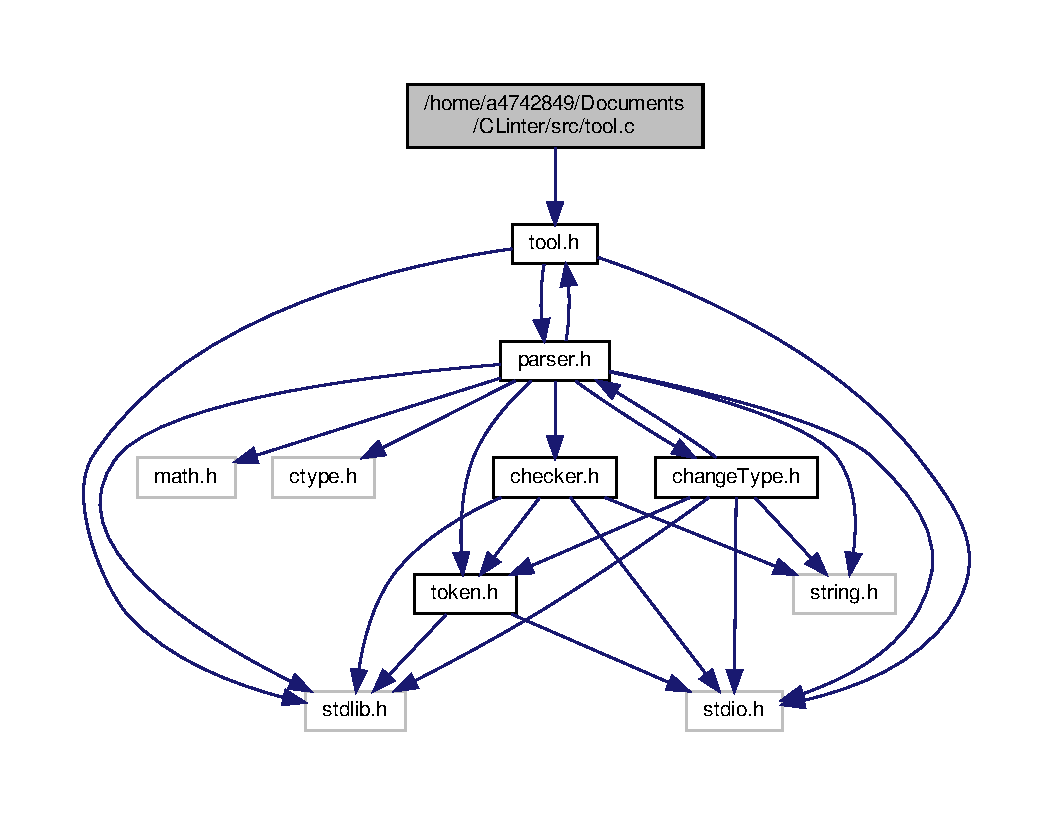
\includegraphics[width=350pt]{tool_8c__incl}
\end{center}
\end{figure}
\subsection*{Functions}
\begin{DoxyCompactItemize}
\item 
void \hyperlink{tool_8c_a57210a98b0bf5cc8f5acbae9f40ad566}{exit\+\_\+m} (char $\ast$message)
\begin{DoxyCompactList}\small\item\em Exit the program with a display message. \end{DoxyCompactList}\item 
void \hyperlink{tool_8c_a87060d093a3121b8c5c6efd5bd073447}{print\+\_\+warning} (char $\ast$message, int line, int pos, char $\ast$file\+Name)
\begin{DoxyCompactList}\small\item\em The main printing function to print warning message with filename and position. \end{DoxyCompactList}\item 
int \hyperlink{tool_8c_a1c6a03ba60a264b76b33280bbddfb926}{is\+Key} (char $\ast$str)
\begin{DoxyCompactList}\small\item\em Tell if string is a C key word. \end{DoxyCompactList}\item 
int \hyperlink{tool_8c_ade60b681643b75ad65527978eb3f8d43}{is\+Num} (char $\ast$str)
\begin{DoxyCompactList}\small\item\em Tell if a string is an Number. \end{DoxyCompactList}\end{DoxyCompactItemize}


\subsection{Detailed Description}
This c file will contain all functions for various tools. 

\begin{DoxyAuthor}{Author}
Antoine T\+A\+V\+E\+R\+N\+I\+ER
\end{DoxyAuthor}
\begin{DoxyDate}{Date}
16/11/2018 
\end{DoxyDate}


\subsection{Function Documentation}
\mbox{\Hypertarget{tool_8c_a57210a98b0bf5cc8f5acbae9f40ad566}\label{tool_8c_a57210a98b0bf5cc8f5acbae9f40ad566}} 
\index{tool.\+c@{tool.\+c}!exit\+\_\+m@{exit\+\_\+m}}
\index{exit\+\_\+m@{exit\+\_\+m}!tool.\+c@{tool.\+c}}
\subsubsection{\texorpdfstring{exit\+\_\+m()}{exit\_m()}}
{\footnotesize\ttfamily void exit\+\_\+m (\begin{DoxyParamCaption}\item[{char $\ast$}]{message }\end{DoxyParamCaption})}



Exit the program with a display message. 


\begin{DoxyParams}{Parameters}
{\em message} & The message displayed in S\+T\+D\+O\+UT \\
\hline
\end{DoxyParams}
\mbox{\Hypertarget{tool_8c_a1c6a03ba60a264b76b33280bbddfb926}\label{tool_8c_a1c6a03ba60a264b76b33280bbddfb926}} 
\index{tool.\+c@{tool.\+c}!is\+Key@{is\+Key}}
\index{is\+Key@{is\+Key}!tool.\+c@{tool.\+c}}
\subsubsection{\texorpdfstring{is\+Key()}{isKey()}}
{\footnotesize\ttfamily int is\+Key (\begin{DoxyParamCaption}\item[{char $\ast$}]{str }\end{DoxyParamCaption})}



Tell if string is a C key word. 


\begin{DoxyParams}{Parameters}
{\em str} & String to check \\
\hline
\end{DoxyParams}
\begin{DoxyReturn}{Returns}
int 0 false else true 
\end{DoxyReturn}
\mbox{\Hypertarget{tool_8c_ade60b681643b75ad65527978eb3f8d43}\label{tool_8c_ade60b681643b75ad65527978eb3f8d43}} 
\index{tool.\+c@{tool.\+c}!is\+Num@{is\+Num}}
\index{is\+Num@{is\+Num}!tool.\+c@{tool.\+c}}
\subsubsection{\texorpdfstring{is\+Num()}{isNum()}}
{\footnotesize\ttfamily int is\+Num (\begin{DoxyParamCaption}\item[{char $\ast$}]{str }\end{DoxyParamCaption})}



Tell if a string is an Number. 


\begin{DoxyParams}{Parameters}
{\em str} & String to check \\
\hline
\end{DoxyParams}
\begin{DoxyReturn}{Returns}
int 0 false else true 
\end{DoxyReturn}
\mbox{\Hypertarget{tool_8c_a87060d093a3121b8c5c6efd5bd073447}\label{tool_8c_a87060d093a3121b8c5c6efd5bd073447}} 
\index{tool.\+c@{tool.\+c}!print\+\_\+warning@{print\+\_\+warning}}
\index{print\+\_\+warning@{print\+\_\+warning}!tool.\+c@{tool.\+c}}
\subsubsection{\texorpdfstring{print\+\_\+warning()}{print\_warning()}}
{\footnotesize\ttfamily void print\+\_\+warning (\begin{DoxyParamCaption}\item[{char $\ast$}]{message,  }\item[{int}]{line,  }\item[{int}]{pos,  }\item[{char $\ast$}]{file\+Name }\end{DoxyParamCaption})}



The main printing function to print warning message with filename and position. 


\begin{DoxyParams}{Parameters}
{\em message} & The message displayed on S\+T\+D\+O\+UT \\
\hline
{\em line} & The line of the warning \\
\hline
{\em pos} & The position of the warning \\
\hline
{\em file\+Name} & The file name location of the warning \\
\hline
\end{DoxyParams}

\hypertarget{tool_8h}{}\section{/home/a4742849/\+Documents/\+C\+Linter/src/tool.h File Reference}
\label{tool_8h}\index{/home/a4742849/\+Documents/\+C\+Linter/src/tool.\+h@{/home/a4742849/\+Documents/\+C\+Linter/src/tool.\+h}}


This header file will contain all required definitions and basic utilities functions to print, check token\textquotesingle{}s nature.  


{\ttfamily \#include $<$stdlib.\+h$>$}\newline
{\ttfamily \#include $<$stdio.\+h$>$}\newline
{\ttfamily \#include \char`\"{}parser.\+h\char`\"{}}\newline
Include dependency graph for tool.\+h\+:\nopagebreak
\begin{figure}[H]
\begin{center}
\leavevmode
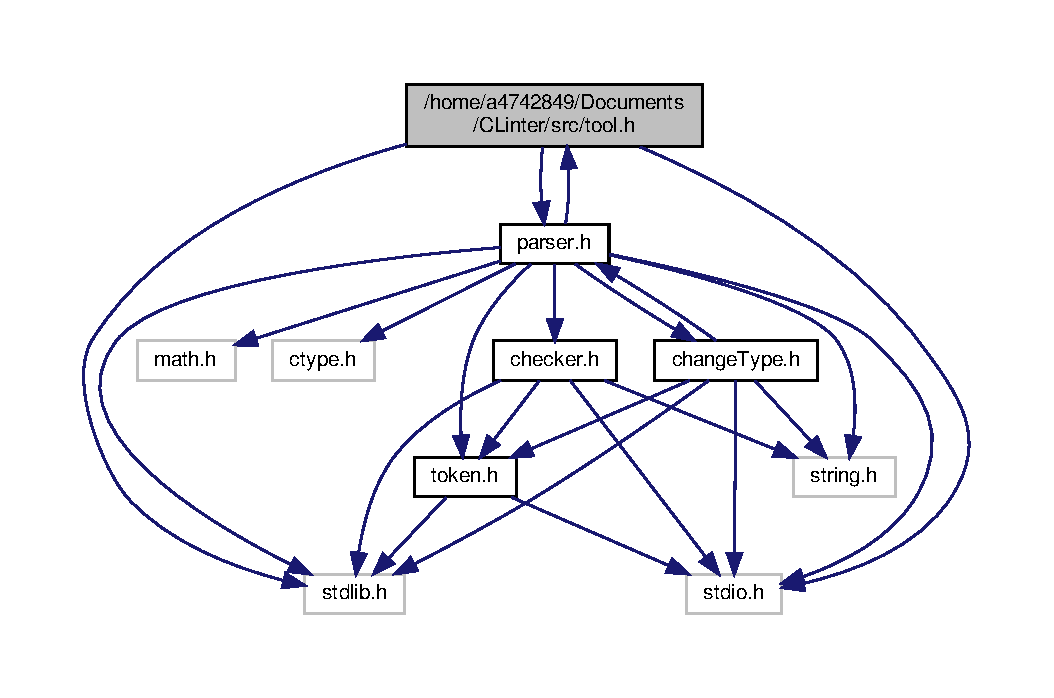
\includegraphics[width=350pt]{tool_8h__incl}
\end{center}
\end{figure}
This graph shows which files directly or indirectly include this file\+:
\nopagebreak
\begin{figure}[H]
\begin{center}
\leavevmode
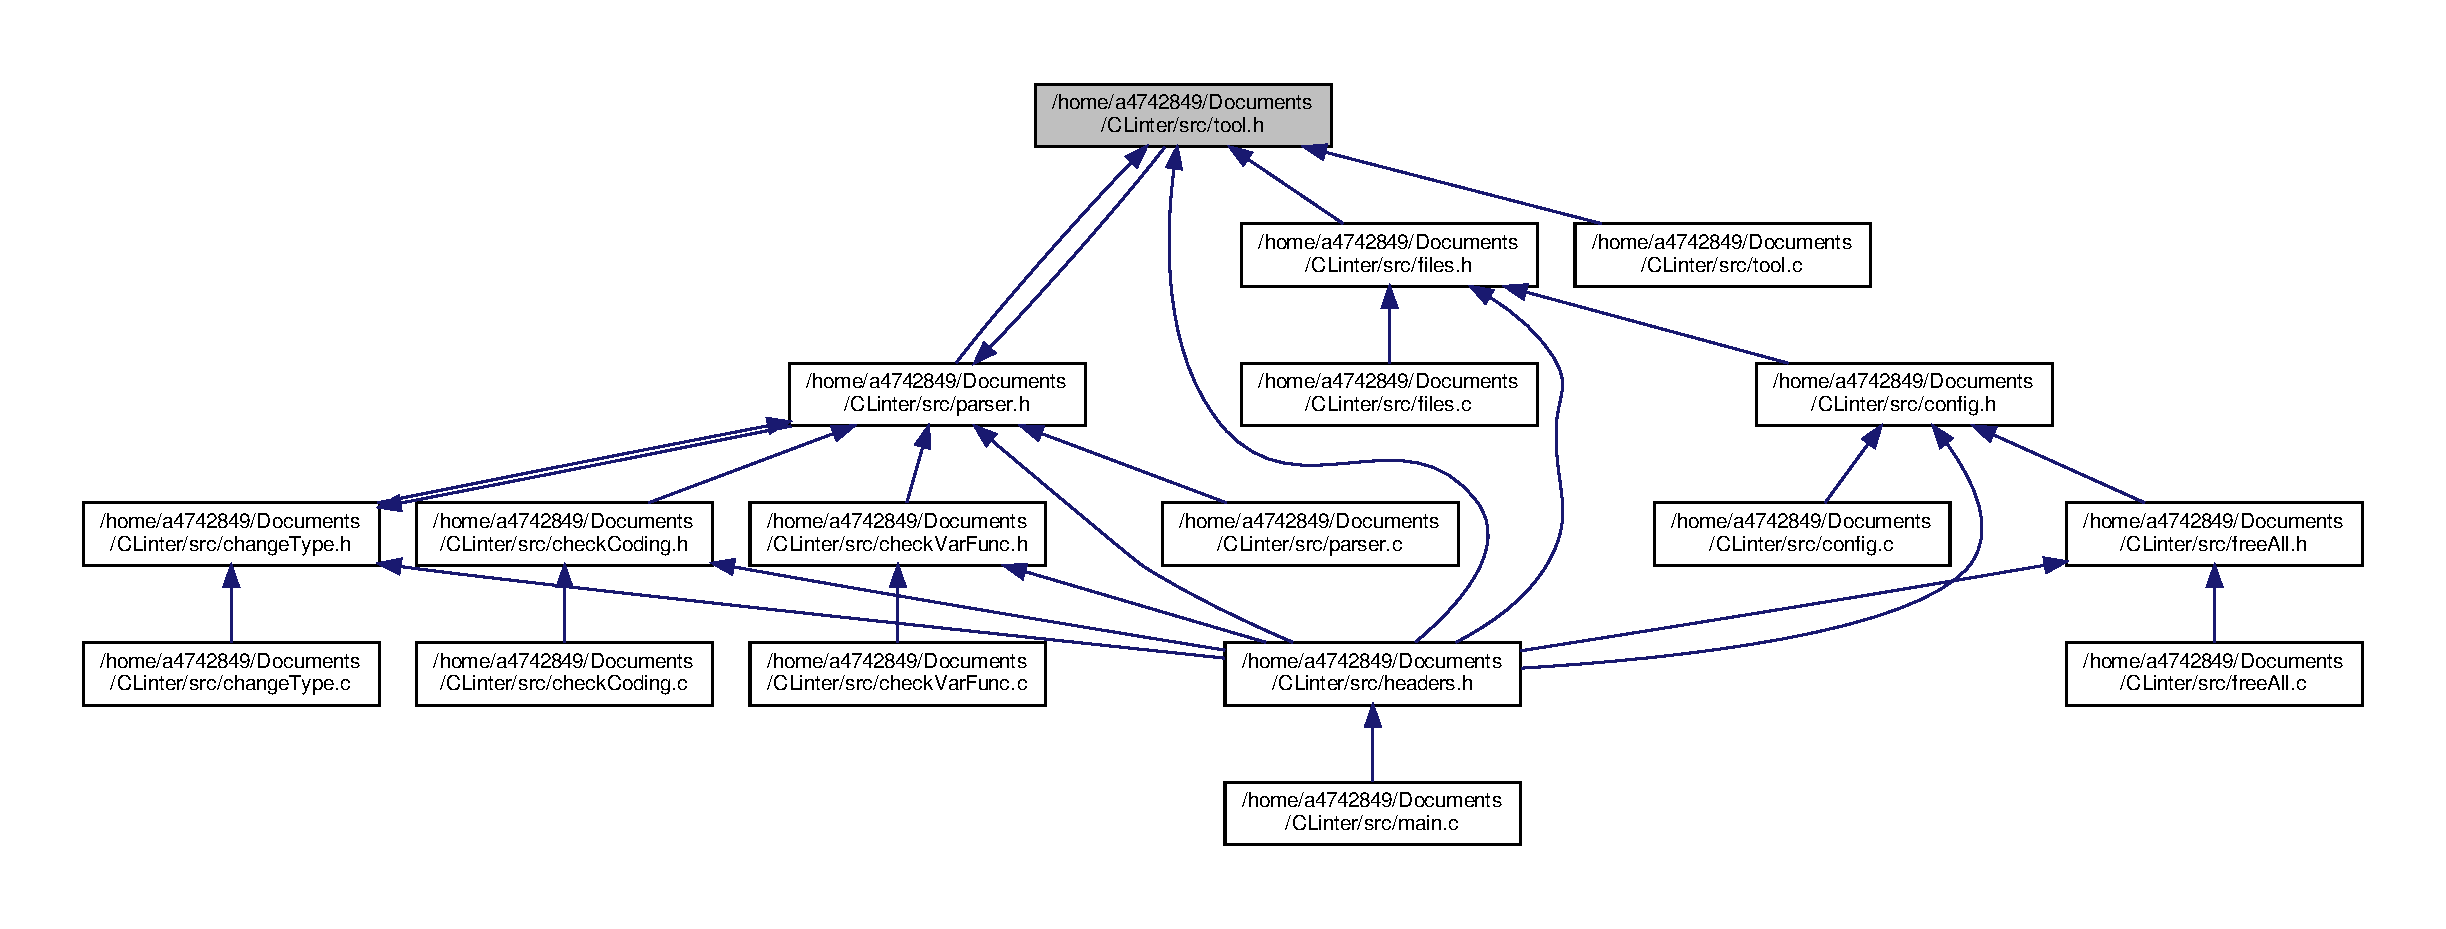
\includegraphics[width=350pt]{tool_8h__dep__incl}
\end{center}
\end{figure}
\subsection*{Functions}
\begin{DoxyCompactItemize}
\item 
void \hyperlink{tool_8h_a57210a98b0bf5cc8f5acbae9f40ad566}{exit\+\_\+m} (char $\ast$message)
\begin{DoxyCompactList}\small\item\em Exit the program with a display message. \end{DoxyCompactList}\item 
void \hyperlink{tool_8h_a87060d093a3121b8c5c6efd5bd073447}{print\+\_\+warning} (char $\ast$message, int line, int pos, char $\ast$file\+Name)
\begin{DoxyCompactList}\small\item\em The main printing function to print warning message with filename and position. \end{DoxyCompactList}\item 
int \hyperlink{tool_8h_a1c6a03ba60a264b76b33280bbddfb926}{is\+Key} (char $\ast$str)
\begin{DoxyCompactList}\small\item\em Tell if string is a C key word. \end{DoxyCompactList}\item 
int \hyperlink{tool_8h_ade60b681643b75ad65527978eb3f8d43}{is\+Num} (char $\ast$str)
\begin{DoxyCompactList}\small\item\em Tell if a string is an Number. \end{DoxyCompactList}\end{DoxyCompactItemize}


\subsection{Detailed Description}
This header file will contain all required definitions and basic utilities functions to print, check token\textquotesingle{}s nature. 

\begin{DoxyAuthor}{Author}
Antoine T\+A\+V\+E\+R\+N\+I\+ER
\end{DoxyAuthor}
\begin{DoxyDate}{Date}
16/11/2018 
\end{DoxyDate}


\subsection{Function Documentation}
\mbox{\Hypertarget{tool_8h_a57210a98b0bf5cc8f5acbae9f40ad566}\label{tool_8h_a57210a98b0bf5cc8f5acbae9f40ad566}} 
\index{tool.\+h@{tool.\+h}!exit\+\_\+m@{exit\+\_\+m}}
\index{exit\+\_\+m@{exit\+\_\+m}!tool.\+h@{tool.\+h}}
\subsubsection{\texorpdfstring{exit\+\_\+m()}{exit\_m()}}
{\footnotesize\ttfamily void exit\+\_\+m (\begin{DoxyParamCaption}\item[{char $\ast$}]{message }\end{DoxyParamCaption})}



Exit the program with a display message. 


\begin{DoxyParams}{Parameters}
{\em message} & The message displayed in S\+T\+D\+O\+UT \\
\hline
\end{DoxyParams}
\mbox{\Hypertarget{tool_8h_a1c6a03ba60a264b76b33280bbddfb926}\label{tool_8h_a1c6a03ba60a264b76b33280bbddfb926}} 
\index{tool.\+h@{tool.\+h}!is\+Key@{is\+Key}}
\index{is\+Key@{is\+Key}!tool.\+h@{tool.\+h}}
\subsubsection{\texorpdfstring{is\+Key()}{isKey()}}
{\footnotesize\ttfamily int is\+Key (\begin{DoxyParamCaption}\item[{char $\ast$}]{str }\end{DoxyParamCaption})}



Tell if string is a C key word. 


\begin{DoxyParams}{Parameters}
{\em str} & String to check \\
\hline
\end{DoxyParams}
\begin{DoxyReturn}{Returns}
int 0 false else true 
\end{DoxyReturn}
\mbox{\Hypertarget{tool_8h_ade60b681643b75ad65527978eb3f8d43}\label{tool_8h_ade60b681643b75ad65527978eb3f8d43}} 
\index{tool.\+h@{tool.\+h}!is\+Num@{is\+Num}}
\index{is\+Num@{is\+Num}!tool.\+h@{tool.\+h}}
\subsubsection{\texorpdfstring{is\+Num()}{isNum()}}
{\footnotesize\ttfamily int is\+Num (\begin{DoxyParamCaption}\item[{char $\ast$}]{str }\end{DoxyParamCaption})}



Tell if a string is an Number. 


\begin{DoxyParams}{Parameters}
{\em str} & String to check \\
\hline
\end{DoxyParams}
\begin{DoxyReturn}{Returns}
int 0 false else true 
\end{DoxyReturn}
\mbox{\Hypertarget{tool_8h_a87060d093a3121b8c5c6efd5bd073447}\label{tool_8h_a87060d093a3121b8c5c6efd5bd073447}} 
\index{tool.\+h@{tool.\+h}!print\+\_\+warning@{print\+\_\+warning}}
\index{print\+\_\+warning@{print\+\_\+warning}!tool.\+h@{tool.\+h}}
\subsubsection{\texorpdfstring{print\+\_\+warning()}{print\_warning()}}
{\footnotesize\ttfamily void print\+\_\+warning (\begin{DoxyParamCaption}\item[{char $\ast$}]{message,  }\item[{int}]{line,  }\item[{int}]{pos,  }\item[{char $\ast$}]{file\+Name }\end{DoxyParamCaption})}



The main printing function to print warning message with filename and position. 


\begin{DoxyParams}{Parameters}
{\em message} & The message displayed on S\+T\+D\+O\+UT \\
\hline
{\em line} & The line of the warning \\
\hline
{\em pos} & The position of the warning \\
\hline
{\em file\+Name} & The file name location of the warning \\
\hline
\end{DoxyParams}

%--- End generated contents ---

% Index
\backmatter
\newpage
\phantomsection
\clearemptydoublepage
\addcontentsline{toc}{chapter}{Index}
\printindex

\end{document}
